\includeonly{settings,HandbuchInc,titel,Kapitel1,Kapitel2,Kapitel3,Kapitel4,Kapitel5,Kapitel6,Quelltexte,ErstellungEigenerMatches}
\documentclass[a4paper,12pt,twoside,halfparskip,bibtotocnumbered,liststotocnumbered]{scrreprt}

\usepackage{ngerman}	%Deutsch
\usepackage[T1]{fontenc}
\usepackage[utf8]{inputenc}

\usepackage{gensymb}	%Sonderzeichen

\usepackage{index}

\newindex{default}{idx}{ind}{E Stichwortverzeichnis}

  
\usepackage{amsmath}	%MAthe
\usepackage{amsfonts}
\usepackage{amssymb}

\usepackage{listings}	%für Quellcode
\usepackage{xcolor}	%für Farben im Quellcode
\lstset{language=[gnu]c++}%language=java}
\lstset{alsolanguage=Java}
\lstset{inputencoding=utf8,
        extendedchars=\true }
\lstset{emph={HashSet,RegionForInterpolation,Face, ConvexHullTreeNode,RegionTreeNode, CHLine, LineDist,LineWA}}
\lstset{stringstyle=\color{blue}}
\lstset{keywordstyle=\color{magenta}\textbf}
\lstset{commentstyle=\color{green}\itshape}
\lstset{breaklines=true,frame=tlrb,frameround=tttt,rulecolor=\color{black},numbers=left,emphstyle=\color{red}\textbf,tabsize=3}

\usepackage{bibgerm}
\usepackage{graphicx}
\usepackage{picins}
\usepackage{ifpdf}
\ifpdf
\DeclareGraphicsRule{*}{mps}{*}{}
\fi

\usepackage{multicol}
\usepackage[german,vlined,boxruled]{/usr/local/teTeX/share/texmf-dist/tex/latex/algorithms/algorithm2e}
\setlength{\algomargin}{1em}
%&\SetInd{1em}{1em}
\Setvlineskip{1em}
\usepackage{framed}
\usepackage{lscape}

\usepackage{units}	%\usepackage{units} 	  	units → Paket für Einheiten: mit \unit[wert]{einheit}, Bsp.: 5 mm \unitfrac[wert]{zähler}{nenner}, Bsp.: 5 g/m \nicefrac[schrift]{zähler}{nenner}

\usepackage[germanb]{minitoc}
\mtcsettitle{parttoc}{Anhangsverzeichnis}
\mtcsetdepth{parttoc}{0}
\mtcsetrules{*}{off} 
\setcounter{tocdepth}{1} %% <- Tiefe bei (Haupt-)Inhaltsverzeichnis

\usepackage{fancyhdr} % für spezielle Kopfzeilen
\usepackage{floatflt}
\pagestyle{fancy}
\setlength{\headheight}{12mm}
\addtolength{\headwidth}{\oddsidemargin}
\addtolength{\headwidth}{\evensidemargin}
\fancyhead[ER,OL]{
\includegraphics[height=1cm]{/home/java/Documents/Tex/Tex/feu_logo2.eps}}
\renewcommand{\chaptermark} [1]{\markboth{ \thechapter.  #1}{ \thesection   #1}}
\fancyhead[EL]{\sc\leftmark }
\fancyhead[OR]{\sc\rightmark}
\lfoot[\thepage]{}
\rfoot[]{\thepage}
\cfoot{}
\renewcommand{\labelenumi}{\theenumi)}
\renewcommand{\labelenumii}{(\alph{enumii})}
\definecolor{red}{rgb}{1,0,0}
\definecolor{RED}{rgb}{1,0,0}
\newcommand{\anmerkung}[1]{{\textit{#1}}}


\usepackage[
dvipdfm,
raiselinks=false,
pdfdisplaydoctitle=true,
breaklinks=true,
 pdfpagelabels=true,
 bookmarks=true,
colorlinks=true,
linkcolor=black,
anchorcolor=black,
citecolor=black,
filecolor=black,
menucolor=black,
urlcolor=black]{hyperref}

\hypersetup{% ä=\344, ö=\366, ü=\374, Ä=\304, Ö=\326, Ü=\334, ß=\377
 pdftitle={Berechnung beweglicher Objekte aus Beobachtungen},
 pdfauthor={Andreas Ruloffs},
 pdfsubject={},
 pdfkeywords={},
 pdfcreator={LaTeX},
 pdfproducer={LaTeX mit hyperref}
}
\begin{document}
%
%       titel.tex - Titelblatt
%
% --- ! Anpassungen sind nur GANZ UNTEN erforderlich !  ---
%
% ---------------------------------------------------------
%       Diese Datei ist Teil der LaTeX-Vorlage fr
%             Studien-und Diplomarbeiten am
%    Institut fr Mechanik und Meerestechnik, TUHH
%
% (c) Institut fr Mechanik und Meerestechnik
%     Technische Universit� Hamburg-Harburg
%     2006
%
% Weitere Informationen finden Sie in  diplomarbeit.tex .
% ---------------------------------------------------------
%
%

% ------------ Definition der Befehle ---------------
%       (hier sind keine Aenderungen noetig !)

% \deckblatt{Rand}{Seitenbreite}{Kopftext}{Fensterbreite}{Fensterhoehe}{Fenstertext}{Untertext}{Fusstext}
%
% Rand:          zusaetzlicher rechter Rand zur Ausrichtung der Seite auf das Sichtfenster
% Seitenbreite:  Seitenbreite
% Kopftext:      Text ueber dem Sichtfenster
% Fensterbreite: Breite des Sichtfensters
% Fensterhoehe:  Hoehe des Sichfensters
% Fenstertext:   Text im Sichtfenster
% Untertext:     Text unter dem Sichtfenster
% Fusstext:      Text nach \vfill

\newcommand{\deckblatt}[8]{
  \begin{titlepage}
  \vspace*{-20mm}
  \hspace{#1}               % Ausrichtung zum Sichtfenster, auch unten
  \begin{minipage}[t]{#2}       % Minipage Titelseite
    \begin{center}
    \begin{minipage}[t][64mm][t]{#2}    % Minipage Kopf
      \begin{center}
      #3
      \end{center}
    \end{minipage} \\           % Minipage Kopf
    \vspace{10mm}
    \begin{minipage}[t][#5][c]{#4}  % Minipage Sichtfenster
      \begin{center}
      #6
      \end{center}
    \end{minipage} \\           % Minipage Sichtfenster
    \vspace{26mm}
    #7
    \end{center}
  \end{minipage} \\         % Minipage Titelseite
  \vfill
  \hspace{#1}               % Ausrichtung der Titelseite zum Sichtfenster
  \begin{minipage}[t]{#2}      % Minipage Datum
    \begin{flushright}
		#8
	\end{flushright}
  \end{minipage}            % Minipage Datum
  \end{titlepage}
}

% \titelseite{Fenstertext}{Untertext}{Fusstext}

\newcommand{\titelseite}[3]{%
  \deckblatt{1mm}{175mm}{
    \vspace*{15mm}    
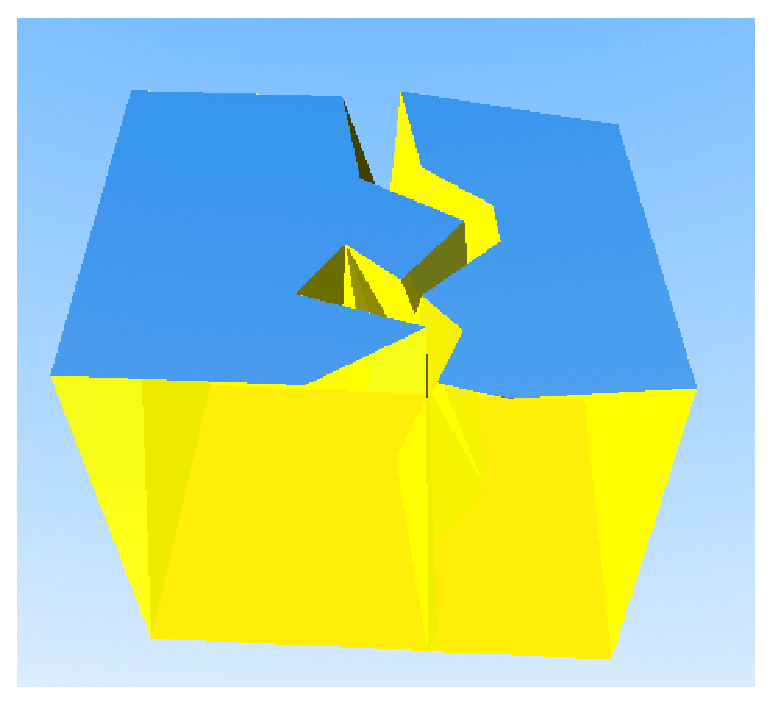
\includegraphics[width=65mm]{/home/java/Documents/Tex/Tex/vrml.eps}
  }{105mm}{65mm}{#1}{#2}{#3}
}

% ------------------ ! Text hier anpassen ! ------------------------

% Schema:  \titelseite{Fenstertext}{Untertext}{Fusstext}
% Fenstertext:   Text im Sichtfenster
% Untertext:     Text unter dem Sichtfenster
% Fusstext:      Text nach \vfill

\titelseite{
  % Fenstertext
  {\large \bf Diplomarbeit} \\  [7mm]
  {\LARGE \bf Berechnung beweglicher Objekte aus Beobachtungen}\\[7mm]
  {vorgelegt von} \\[7mm]
  {\large Andreas Ruloffs}\\
  {\large 6~65~11~19}
}{
  % Untertext
\begin{flushright}
  Betreuer: \\[5mm]
  Prof. Dr.Ralf Hartmut G"uting \\[12mm]
   \begin{floatingfigure}[r]{20mm}
      
\includegraphics[width=20mm]{/home/java/Documents/Tex/Tex/feu_logo2.eps}
   \end{floatingfigure}
\textbf{FernUniversit"at}\\
Gesamthochschule Hagen\\
Fachbereich Informatik\\
Lehrgebiet Praktische Informatik IV
\end{flushright}
}{
  % Fusstext
 Gelsenkirchen, M"arz 2008}

\begin{abstract}
Diplomarbeit halt
\end{abstract}
\dominitoc[e]
\doparttoc

\tableofcontents 

%


\chapter[Einleitung \anmerkung{ca. 5 Seiten}]{Einleitung\\
\normalsize{(kuze Einleitung, was ist Secondo, warum MovinRegions, warum Interpolation) \anmerkung{ca. 5 Seiten}}} \label{Kapitel1}
\anmerkung{Beschreibung der allgemeinen Problemstellung, man m"ochte Moving-Regions darstellen k"onnen z. B. f"ur die Deter Daten, Kurzbeschreibung dieser Daten, das f"uhr zu Secondo, und den Moving-Regions in Secondo. Die Schwierigkeiten bie der Erstellung von diesen, und die Struktur der Deter-Daten f"uhren zu dem Interpolations-Problem, dass im folgenden gel"oste dwerden soll.}


%\minitoc
%\newpage
%\section{Secondo \anmerkung{2 Seiten}}
%\subsection{Was ist Secondo}
%\anmerkung{Eine kuze Beschreibung, was Secondo ist, Die Entstehungsgeschichte und was Secondo so alles kann.}
%\section{Moving Regions \anmerkung{2 Seiten}}
%\anmerkung{Eine kurze Beschreibung, was Moving-Regions sind, und eine Beschreibung wozu diese gut sind. Eventuell k"onnte ich %hier das Flugzeugbeispiel benutzen}
%\subsection{Was sind Moving Regions?}

%\subsection{Wof"ur sind Moving Regions gut?}

%\section{Interpolation \anmerkung{1 Seite}}
%\anmerkung{Warum die Erzeugung von Moving-Regions kompliziert ist, und inwiefern diese Problemetik sich duch meine Arbeit verbesesrn wird.}
%\subsection{Was sind die Probleme bei der Erstellung von Moving Regions?}
%\subsection{Wie sieht die L"osung aus?}

\chapter[Darstellung der Grundlagen \anmerkung{30-40 Seiten}]{Darstellung der Grundlagen\\
\normalsize{(nicht selbstgemachtes
SECONDO,
MovingRegion,
T\o{}ssebro)}\anmerkung{30-40 Seiten}} \label{Kapitel2}
\minitoc
\newpage
\section{SECONDO \anmerkung{10 Seiten}}\label{SecondoEinfuehrung}

\subsection{Einführung}
SECONDO ist ein erweiterbares Datenbank"-management-System (DBMS), das von dem Lehrgebiet Praktische Informatik IV, ,,Datenbanksysteme für neue Anwendungen'' in der Fakultät Mathematik und Informatik der Fernuniversität Hagen entwickelt wurde, und wird.

Das Ziel von SECONDO ist es, einen ,,allgemeinen'' Datenbanksystemrahmen zur Verfügung zu stellen, der mit Implementierungen von verschiedenen DBMS Datenmodellen gefüllt werden kann.

Zum Beispiel sollte es möglich sein, relationale, objektorientierte, zeitliche, oder XML-Modelle zu implementieren und Datentypen für räumliche Daten, bewegte Objekte, graphentheoretische Strukturen oder Schachspiele unterzubringen. Die Möglichkeit zur Änderung des grundlegenden Datenmodelle sind eine Besonderheit von SECONDO. Für die Erweiterbarkeit des System sind die ,,SECONDO-Algebren'' zuständig, deren Konzept ich weiter unter näher beleuchte.

Das SECONDO-System setzt sich im wesentlichen aus drei Komponenten zusammen.
\begin{enumerate}
\item Der Kernel

Der Kernel ist für die Datenhaltung und für die Abfragebearbeitung in dem speziellen SECONDO-Syntax zuständig. Datenpersistenz erreicht der Kernel durch das Zusammenspiel mit einer BerkleyDB. Die Algebren zur Unterstützung verschiedener Datentypen werden in den Kernel gehängt. Der Kernel, und die meisten Algebren sind in C++ geschrieben, es gibt aber auch die Möglichkeit Algebren in Java zu kodieren.

\item Der Optimizer

Der Optimizer bietet die Möglichkeit Datenbankanfragen in einem eigenen, SQL-ähnlichen Syntax zu formulieren. Der Optimizer findet für diese Abfragen eine optimale Ausführung, indem er etwa den besten Join-Typ einer Abfrage findet, oder die Reihenfolge der Abarbeitungen optimiert. Der Optimizer ist in PROLOG geschrieben. Die vorliegende Arbeit benötigt die Möglichkeiten des Optimizers nicht.

\item Das GUI

Das SECONDO-GUI bietet eine komfortable Möglichkeit entweder direkt, oder  über den Optimizer  auf den Kernel zuzugreifen. Analog zu der Erweiterbarkeit des Kernels durch Algebren ist auch das GUI, durch so genannte Viewer, erweiterbar. Diese Viewer bieten die Möglichkeit, neue Datentypen auch darzustellen. Da in dieser Arbeit keine neuen Datentypen eingeführt werden und sich die verwendeten Datentypen alle im ,,Hoese-Viewer'' darstellen lassen, war eine Erweiterung des GUI nicht notwendig. Man wird jedoch im Laufe dieser Arbeit öfter Grafiken finden, die unter Zuhilfenahme des GUI entstanden sind. Das GUI ist in Java geschrieben, und auch in dieser Sprache erweiterbar.

\end{enumerate}

Eine Datenbank in SECONDO ist nichts weiteres als eine Menge von SECONDO-Obje"-kten. Nur wenn der Anwender diese Objekte in Relationen verwaltet, was meistens der Fall ist, weißt die Datenbank eine Form auf, wie man diese von relationalen Datenbanken gewohnt ist.

Um Daten zwischen den einzelnen Komponenten austauschen zu können, wird das NestedList-Format benutzt. Eine NestedList ist eine geschachtelte Liste von elementaren Datentypen, deren Schachtelungstiefe unbegrenzt ist. Eine große NestedList wird zum Beispiel auch benutzt, um eine Datenbank in eine Datei zu exportieren, beziehungsweise eine solche Datei wieder einzulesen. Das Framework rund um SECONDO bietet dem Programmieren die Möglichkeiten NestedLists relativ einfach handhaben zu können.

\subsection{Das Konzept der SECONDO-Algebren}

Eine SECONDO-Algebra erweitert das System um neue Datentypen, und die Operationen, welche auf diesen durchführbar sind. Es kann aber auch Algebren geben, die entweder nur Datentypen, oder nur Operatoren bereitstellen. Die Algebra, welche im Zuge dieser Arbeit erstellt wird besteht zum Beispiel nur aus einem einzigen Operator.

Bei der Herstellung von Datenpersistenz und der Einbettung in das SECONDO-System nehmen dem Programmierer einige Schnittstellen den Großteil der Arbeit ab.

Möchte dieser einen neuen Datentyp implementieren, so muss er sich zuerst eine Repräsentation seiner Daten in einer NestedList überlegen, und Methoden implementieren, diese aus seinen Objekten zu erzeugen, beziehungsweise Objekte aus der NestedList wiederherzustellen\footnote{Es gibt sogar die Möglichkeit zwei  verschiedene NestedList Formate für die Kommunikation mit den anderen Komponenten und für die interne Speicherung zu definieren. Das ist aber im Rahmen dieser Arbeit nicht weiter von Belang.}. Hierdurch ist bereits die Datenpersistenz gewährleistet.

Wichtiger für diese Arbeit jedoch ist die Implementierung eines neuen Operators. Um einen Operator zu schreiben muss man im Wesentlichen zwei Funktionen schreiben, die TypeMapping-Funktion und die ValueMapping-Funktion. Zusätzlich kann es es noch eine Selection-Funktion geben, die die Implementierung von überladenen Operatoren ermöglicht.

Die TypeMapping-Funktion überprüft ob die eingehenden Daten der Funktionsspezifikation entsprechen, und gibt den Typ des noch zu berechnenden Ergebnisses zurück, falls dies der Fall ist. Sollten die eingehenden Daten nicht das erwartete Format haben, kann die TypeMapping-Funktion die weitere Abarbeitung abbrechen, indem sie dem System einen ,,typeerror'' liefert.

Ist die Type"-Mapping-Funktion erfolgreich ausgeführt worden, so kann man in der Value"-Mapping-Funktion die eingehenden Daten lesen, und aus diesen das gewünschte Ergebnis berechnen.


\subsection{Einige wichtige Algebren}

Im folgenden stelle ich einige Algebren vor, die im Laufe der Arbeit von besonderem Interesse sind. 

\subsubsection{StandardAlgebra}
Die Standart-Algebra beinhaltet die Unterstützung einiger wichtiger grundlegenden Datentypen. Diese sind:
\begin{itemize}
\item int

Der Datentyp für Ganzzahlen.
\item real

Der Datentyp für Fließkommazahlen. Hier ist zu beachten, dass SECONDO zwischen ganzen Zahlen und Fließkommazahlen streng unterscheidet. Möchte man etwa 1 als Fließkommazahl behandeln, so muss man zwingend 1.0 schreiben.
\item bool

Der Datentyp für Wahrheitswerte. Diese werden als ,,TRUE'' oder ,,FALSE'' ausgedrückt.
\item string

Eine Zeichenkette mit höchstens 48 Zeichen. Eine Unterstützung von regionalen Zeichensätzen ist nicht gegeben.
\end{itemize}

Für die nummerischen Datentypen stehen grundlegende nummerische Operationen, wie Addition, Division oder auch Logarithmenbildung oder die Quadratwurzelfunktion zur Verfügung.

An elementaren Stringoperationen stehen zum Beispiel Konkatenierung, Vergleich, Suchen in Strings oder Extraktionen, bereit.

\subsubsection{RelationAlgebra}

Diese Algebra stellt einige der wichtigsten Datentypen und Operationen bereit, welche man von relationalen Datenbanksystemen kennt.
 
\begin{itemize}
\item tuple

Ein Datentyp für ein Tupple von Objekten. Etwa das Tuppel:\\ \verb+(tuple((name string)(age int)))+ kann mit den Daten \verb+("Myers" 53)+ gefüllt werden.
\item rel

Ein Datentyp für eine Relation von Tuppeln. Das Beispiel von oben kann man erweitern, zu \verb+(rel(tuple((name string)(age int))))+. Diese Relation kann mit den Daten \verb+(("Myers" 53)("Smith" 21))+ gefüllt werden.
\end{itemize}
Die Operationen, die diese Algebra bereitstellt sind die, welche man von relationalen Datenbanken kennt, und die nur eine einzige Tabelle betreffen.

Dies sind zum Beispiel Projektion, Erweiterung um ein Attribut, Selektion oder Kartesische Produkt \footnote{Dies passt hier nicht so ganz, da hier mehrere Tabellen betroffen sind, der Operator ist aber trotzdem in dieser Algebra zu finden.}.

\subsubsection{ExtRelationAlgebra}

Diese Algebra stellt keine weiteren Datentypen zur Verfügung, sondern ergänzt das System um weitere Operationen auf Relationen und Tuppeln. Tendenziell finden sich in dieser Algebra diejenigen Operationen, welche auf mehreren Relationen agieren.

Speziell verschiedene Join- und Union-Verfahren, aber auch Operationen zum Gruppieren, Sortieren und Aggregieren von Daten sind hier zu finden.

\subsubsection{SpatialAlgebra}
In dieser Algebra werden geometrische und geographische Objekte verwaltet.
\begin{itemize}
\item point

Dieser Datentyp beschreibt einen Punkt im $\mathbb{R}^2$ oder im $\mathbb{N}^2$.
\item points

Dieser Datentyp beschreibt eine Menge von unverbundenen, zweidimensionalen Punkten. 
\item line

Dieser Datentyp beschreibt ein Liniensegment zwischen zwei Punkten.
\item region

Dieser Datentyp repräsentiert eine Region. Eine Region ist eine, durch mehrere Polygone beschriebene, Fläche.
\end{itemize}

In dieser Algebra finden sich Operationen auf den geometrischen Objekten. Zum Beispiel sind das:
,,enthalten sein'', Schnitte, Abstände, Flächenberechnung, Skalieren oder Verschieben.
 
Die interne Repräsentation dieser Daten besteht aus Halbsegmenten, einem Datentyp welcher sich besonders gut zur Verarbeitung durch Sweep-Line-Verfahren eignet.

\subsubsection{PlaneSweepAlgebra}

Diese Algebra stellt keine eigenen Datentypen zur Verfügung, sondern bietet weitere Operationen auf den Datentypen der SpatialAlgebra an.

Die Operationen sind solche, die sich mittels eines Sweep-Line-Verfahrens lösen lassen. Etwa Vereinigungen, Durchschnitte und Differenzen von Regionen oder Schnittpunktberechnungen.

\subsubsection{PlugJoinAlgebra}

Auch diese Algebra stellt keine Datentypen zur Verfügung, sondern ergänzt einen einzigen Operator, nämlich ,,spatialjoin''.

Dieser dient dazu, ein Join zwischen geometrischen Daten herzustellen. Das Kriterium zum Erstellen des Joins ist hierbei die Überlappung der geometrischen Daten. 

\subsubsection{DateTimeAlgebra}
\begin{itemize}
\item instant

Dies ist ein Datentyp, mit welchem sich ein Zeitpunkt definieren lässt. Man kann in verschieden Genauigkeitsstufen ein Datum angeben (von Jahr-genau bis zu Millisekunden-genau).
\item duration

Dieser Datentyp dient der Verwaltung von Zeitdauern.
\end{itemize}

An Operationen bietet diese Algebra verschiedene Möglichkeiten der Datumserzeugung und der Datumsaritmetik an. Zum Beispiel die Extraktion von Datumteilen, oder die Addition von Tagen auf ein Datum.

\subsubsection{GraphAlgebra}

Diese Algebra ergänzt SECONDO um die Möglichkeit Graphen zu verwalten. Die dazugehörigen Datentypen sind:

\begin{itemize}
\item vertex

Eine Ecke in eines Graphen oder eines Pfads.
\item edge

Dieser Datentyp repräsentiert eine Kante eines Graphen oder eines Pfades.
\item graph

Mit Hilfe dieses Datentyps lassen sich Graphen verwalten.
\item path

Dieser Datentyp repräsentiert einen Pfad.
\end{itemize}

Die Algebra enthält Operatoren, mit deren Hilfe sich zum Beispiel Graphen konstruieren lassen, kürzeste Pfade mittels des Djiksta-Algorithmuses finden lassen oder Zusammenhangskomponenten finden lassen.

\subsubsection{TemporalAlgebra}

Diese Algebra dient dazu einige einfache sich verändernde Datentypen zu verwalten. Eine Beschreibung dieser Datentypen findet sich unter \cite{FGNS}.
\begin{itemize}
\item rint

Dieser Datentyp repräsentiert Mengen von Intervallen auf den ganzen Zahlen.
\item rreal

Dieser Datentyp repräsentiert Mengen von Intervallen auf Fließkommazahlen.
\item periods

Dieser Datentyp repräsentiert Mengen von Zeitintervallen.
\item ibool

Mit Hilfe dieses Datentyps lassen sich Paare von einem boolschen Werte und einem Zeitpunkt verwalten.
\item iint

Mit Hilfe dieses Datentyps lassen sich Paare von einer ganzen Zahl und einem Zeitpunkt verwalten.
\item ireal

Mit Hilfe dieses Datentyps lassen sich Paare von einer Fließkommazahl und einem Zeitpunkt verwalten.
\item ipoint

Mit Hilfe dieses Datentyps lassen sich Paare von einem Punkt und einem Zeitpunkt verwalten.
\item ubool

\item uint

\item ureal

\item upoint

\item mbool

\item mint

\item mreal

\item mpoint

Dieser Datentyp dient der Verarbeitung eines Punktes, der sich über der Zeit verändert.
\end{itemize}



\subsection{Die MovingRegionAlgebra}
Da diese Algebra für meine Arbeit besonders wichtig ist, beschreibe ich diese ausführlicher.

Diese Klasse wurde im Zuge einer Abschlussarbeit \cite{Mue} im Studiengang Bachelor of Science im Fach Informatik  erstellt.

\begin{itemize}
\item intimeregion

Dieser Datentyp dient dazu Paare von Regionen und Zeitpunkten zu verwalten. Dieses Konstrukt dient besonders zur Verwaltung von Schnappschüssen zu bestimmten Zeitpunkten.
\item uregion

Mit Hilfe dieses Datentyps lassen sich Regionunits verwalten. Eine Regionunit dient dazu, eine kontinuierliche Bewegung einer Region zu einem Zeitpunkt in eine andere Region zu einem späteren Zeitpunkt darzustellen. 
\item movingregion

Dies ist die Repräsentation einer MovingRegion. Eine MovingRegion ist eine Menge von Regionunits, bei denen alle Zeitintervalle paarweise disjunkt sind. 
\end{itemize}

Eine formelle Definition von MovingRegion und Regionunit werde ich etwas später, unter \ref{DatenMoving}, geben.

Es existieren Operationen, mit deren Hilfe man Fragen zu bestehenden MovingRegion und Regionunits beantworten kann, etwa ob ein MovingRegion irgendwann einen Punkt berührt, oder wann ein Movingpoint sich in einer MovingRegion befindet, es fehlen aber noch Methoden um einfach MovingRegions zu erzeugen. 
 
\section{Das Paper von Erlend T\o{}ssebro \anmerkung{10 Seiten}}\label{Tossebro}

Eine der wichtigsten Grundlagen der vorliegenden Arbeit ist das Paper: ,,Creating Repesentations for Continuously Moving Regions from Observations'' \cite{TG} von Erlend T\o{}ssebro und Ralf Hartmund G"uting \cite{TG}, in dem die Autoren sich mit den theoretischen Grundlagen des Problems besch"aftigt, und L"osungsvorschl"age zu vielen der vorkommenden Teilprobleme gemacht haben.

Im Rahmen dieses Projektes ist auch eine Java-Applikation entstanden, welche im Rahmen meiner Arbeit erweitert wurde.

\subsection{Die zugrundeligenden Datentypen}\label{DatenMoving}
Nach der allgemeinen Einleitung skizzierten die Autoren kurz die Datentypen, wie diese in \cite{FGNS} beschrieben sind.

Zuerst die nicht beweglichen Daten:
$$Seg=\{(u,v)|u,v\in Point, u<v\}$$

Ein Segment ist also ein Liniensegment zwischen zwei Punkten. 

$$Cycle=\{S\subset S\}$$

Ein Cycle ist eine Menge von Liniensegmenten, die zusammen ein einfaches Polygon bilden müssen.

$$Face=\{(c,H)|c\in Cycle, H \subset Cycle\}$$

Ein Face setzt sich aus einem Cycle, der äußeren Begrenzungslinie, und einer Menge von anderen Cycles, den Löchern oder Holes zusammen. Jedes Hole muss komplett innerhalb des äußeren Cycles liegen, und zwei Holes dürfen sich nicht überschneiden. 

$$Region=\{F\subset Face|f_1,f_2\in F \wedge (f_1\neq f_2) \Rightarrow \text{Kanten von }f_1\text{ und } f_2 \text{ sind disjunkt. } \}$$

Eine Region schließlich setzt sich aus mehreren Faces zusammen, wobei sich diese nicht überschneiden dürfen. 

Nun skizzieren die Autoren die beweglichen Datentypen:

$$MPoint=\{(x_0,x_1,y_0,y_1)|x_0,x_1,y_0,y_1\in \mathbb{R}\}$$

Ein MovingPoint setzt sich aus zwei Punkten, dem Start- und dem Endpunkt zusammen.

$$MSeg=\{(s,e)|s,e\in MPoint\}$$

Ein MovingSegment setzt sich aus zwei MovingPoints zusammen, wobei aber alle vier beteiligten Start- und Endpunkte auf einer Ebene liegen müssen. Ein wichtiger Sonderfall des MovingSegements ist der, wenn beide Start- oder beide End-punkte zusammenfallen. In diesem Fall repräsentiert ein MovingSegment ein Dreieck in drei Dimensionen.

$$MCycle=\{(s_0,s_1,\hdots ,s_{n-1})|n\geq3, s_i\in MSeg\}$$

Ein MovingCycle ist die bewegliche Version eines Cycles. Die beteiligten MovingSegements müssen zusammen eine geschlossene, dreidimensionale Struktur bilden.

$$MFace=\{(c,H)|c\in MCycle, H\subset MCycle\}$$

Ein MovingFace ist die dreidimensionale Version eines Faces, und setzt sich analog zu diesem zusammen.

$$URegion=\{(i,F)|i\in Intervall, F\subset MFace\}$$

Eine RegionUnit schließlich besteht aus einer Menge von MovingFaces und einem Zeitintervall. 

Eine MovingRegion schließlich besteht aus mehreren RegionUnits, bei denen die Zeitintervalle paarweise disjunkt sind.

\subsection{Der Rotating-Pane-Algorithmus}

Die Autoren entwickeln einen Algorithmus, mit dessen Hilfe sich MovingCycles aus zwei konvexen Polygonen berechnen lassen. Anschaulich funktioniert dieser Algorithmus wie folgt:

Wähle eine Kante $s$ des einen Polygons, und lasse die Grundebene des Polygons entlang dieser Achse rotieren. Die Ebene wird dann auf das andere Polygon treffen. Trifft die Ebene zuerst auf einen einzigen Punkt $T$, so gehört das Dreieck aus den beiden Punkten von $s$ und $T$ zu dem MovingCycle.

Trifft die Ebene aber auf eine Kante $t$, so gehört das MovingSegment von $s$ zu $t$ zu dem MovingCycle.

Dieses Verfahren wende auf alle Kanten aus beiden Polygonen an.

Die Autoren geben auch noch einen Algorithmus an, der diese Idee weiterverfolgt, der aber technisch einfacher zu implementieren ist. Eine leicht veränderte Version dieses Algorithmuses beschreibe ich unter \ref{rotPane} genauer.

Die Autoren geben noch die Laufzeit des Verfahrens an und sagen, dass der Algorithmus zu zwei Polygonen, welche zusammen $n$ Ecken haben, ein MovingCycle berechnet und hierfür $O(n*\log{n})$ Zeit benötigt. Liegen die Punkte der Polygone bereits sortiert vor, so sinkt die Laufzeit auf $O(n)$.

Die Autoren räumen ein, dass dieses Verfahren nicht gut mit Rotationen umgehen kann. Lassen wir etwa zwei dünne Rechteck durch diesen Algorithmus laufen, die um 90\degree gedreht sind, so wird die Interpolation nach der Hälfte der Zeit ungefähr quadratisch  sein und einen zu großen Flächeninhalt aufweisen. Abbildung~\ref{fig:BeispielschlechteRot} zeigt dieses Beispiel. Eine Lösung dieses Problems können die Autoren nicht angeben, bei Rotationen sollten also die Unterschiede zwischen den Schnappschüssen nicht zu groß sein.

\begin{figure}
	\centering
	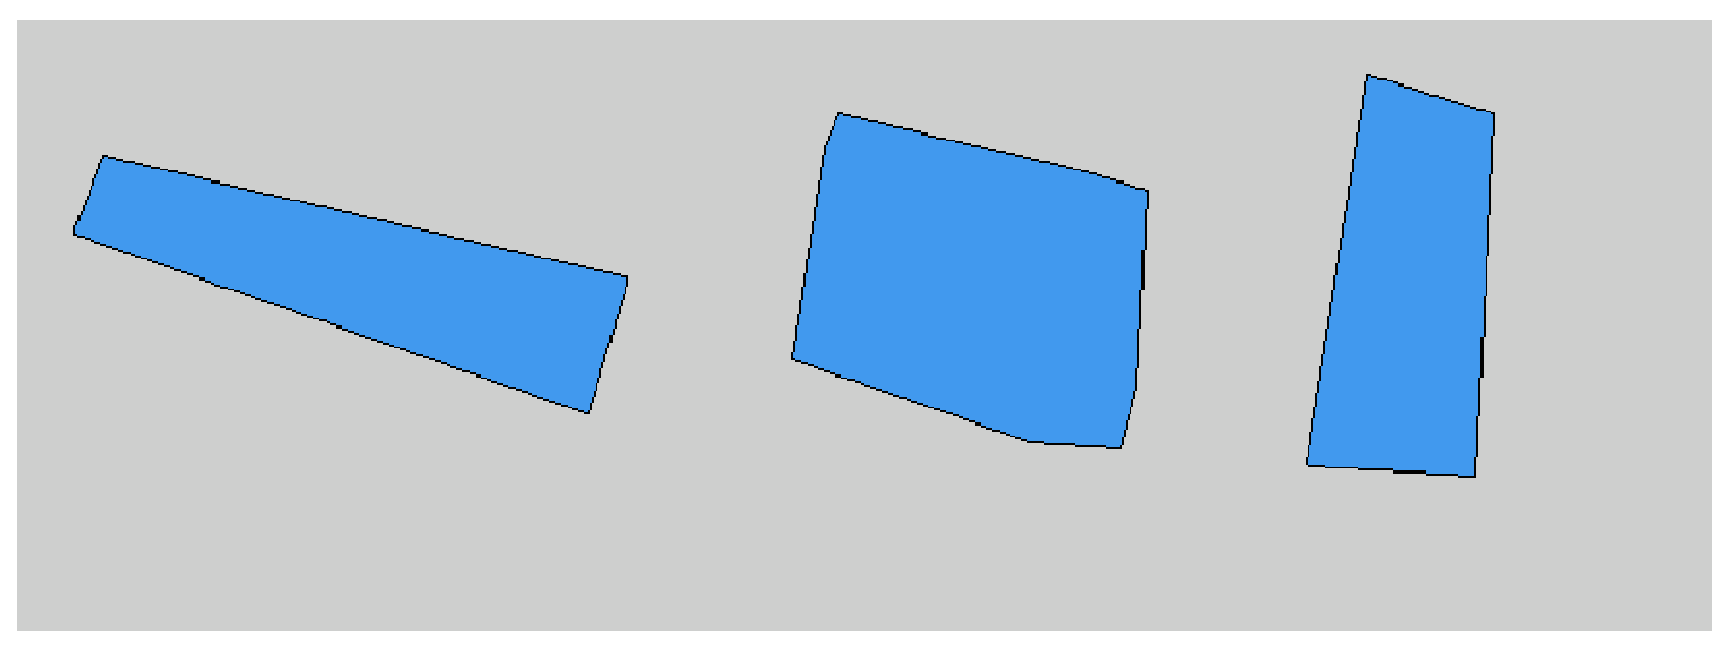
\includegraphics[scale=0.6]{Rotation.eps}
	\caption{Ein Beispiel in dem man die Schwäche des Verfahrens bei großen Rotationen sehen kann.}
	\label{fig:BeispielschlechteRot}
\end{figure}

\subsection{Der Konvexe Hüllenbaum}

Das obige Verfahren kann nur mit konvexen Polygonen umgehen. Um im Allgemeinen einfache Polygone bearbeiten zu können führen die Autoren den ConvexHullTree ein. Die Idee hinter diesen ist es, einfache Polygone als konvexe Polygone mit konvexen Löchern aufzufassen. 

Ein ConvexHullTreeNode ist ein konvexes Polygon, bei dem jeder Kante wiederum ein ConvexHullTreeNode zugeordnet werden kann. Diese Kinderelemente werden von dem Vaterelement abgezogen. Abbildung~\ref{fig:ConHullTree} zeigt einen solches Konstrukt.

\begin{figure}
	\centering
	
\includegraphics{feu_logo2.eps}
	\caption{Ein Beispiel für einen ConvexHullTree.}
	\label{fig:ConHullTree}
\end{figure}

Die Autoren beschreiben, wie man einen solchen Baum aufbaut. Dieses Verfahren ist näher unter \ref{constCHTN} beschrieben.

Die Komplexität der Konstruktion eines Hüllenbaumes wird mit $O(dn*\log(n))$ angegeben, wobei $d$ die Tiefe des resultierenden Baumes ist.

Der umgekehrte Weg, also aus einem ConvexHullTree wieder ein Polygon zu erzeugen funktioniert so:

\begin{itemize}
\item Gebe jedes Segment zurück, für das es kein Kindelement gibt.
\item Für jedes Segment, welches ein Kindelement hat benutze diese Funktion rekursiv.
\end{itemize}

\subsection{Matching zweier Regionen}

Im Weiteren beschäftigen sich die Autoren mit der Frage, wie man zu gegebenen Polygonen, welche die beiden Schnappschüsse einer MovingRegion darstellen sollen, ein Match bestimmen kann. Ein Match ist eine Menge von Paaren von Cyclen, die zusammengehören.

Die Autoren unterscheiden drei unterschiedliche Arten von Matches:

\begin{itemize}
\item Wenn beide Regionen aus mehreren Faces zusammengesetzt sind, welche Faces auf der einen Seite passen dann zu welchen Faces auf der anderen Seite?
\item Falls ein Face mehrere Holes hat, welches Hole auf der einen Seite passt dann zu welchem Hole auf der anderen Seite?
\item Hat ein Cycle mehrere Konkativitäten, welche Konkativitäten auf der einen Seite passen dann zu welchen Konkavitäten auf der anderen Seite?
\end{itemize}

In all diesen Fällen ist auch noch zu beachten, dass einzelne Objekte verschwinden können, oder das mehrere auf der einen Seite zu einem Objekt auf der anderen Seite verschmelzen können.

Um die Qualität eines Matches bestimmen zu können, geben die Autoren einige Kriterien an:

\begin{enumerate}
\item Ein matching-Verfahren sollte das korrekte Ergebnis liefern, falls beide Schnappschüsse übereinstimmen.
\item Komponenten, die sich relativ zu ihrer Größe wenig bewegt haben, sollten korrekt gematcht werden können.
\item Komponenten die nur kleine Änderungen an Größe und Form erfahren haben sollten korrekt gematcht werden.
\item Ein Matching-Verfahren sollte Komponenten erkennen, die sich in mehrere neue aufgesplittet haben, oder solche die sich vereinigen.
\item Ein Matching-Verfahren sollte Kriterien anbieten um zu entscheiden, ob zwei Momentaufnahmen gut zueinander passen, oder ob der zeitliche Abstand zwischen diesen zu groß gewählt ist.
\end{enumerate}

Die Autoren führen den Begriff des ,,sicheren'' Matches an:

Sei $mr$ eine MovingRegion und seien $S_1$ und $S_2$ zwei Schnappschüsse dieser MRegion zu den Zeitpunkten $t$ und $t+\Delta t$. Ein Matching-Verfahren ist sicher zu nennen, falls es ein $\epsilon >0$ gibt, so dass das Match korrekte Ergebnisse liefert, für alle $\Delta t < \epsilon$.

Die Autoren finden drei verschiedene Matching-Strategien, die im folgenden kurz aufgef"uhrt werden:
\begin{enumerate}
\item Position of centroid \label{MatchSchwer}

Bestimme den Schwerpunkt jedes Cycles,  bilde aus diesem einen gewichteten Graphen, mit den Entfernungen als Kantengewichte und suche in diesem "`N"achste Nachbarn"'.
\item Fixed threshold (set of cycles)\label{fixedThre}

Matche zwei Cycles, wenn sie sich wechselseitig  mehr als threshold (in \%) überlappen.

\item Maximize Overlap (set of cycles)

Bilde einen gewichteten Graphen, in dem die Cycles Knoten sind, und dessen Kanten mit dem Grad der Überlappung gewichtet sind. Matche dann ein Cycle $c$ mit demjenigen, mit dem er die gr"o"ste Überlappung aufweist, und mit allen, f"ur die $c$ der Cycle mit der gr"o"sten Überlappung ist.
\end{enumerate} 

Die Autoren kommen zu dem Schluss, dass das Schwerpunktverfahren kein sicheres Verfahren sei, da der Schwerpunkt eines Polygons außerhalb dieses liegen kann.

Im weiteren Verlauf betrachten die Autoren nur noch einzelne Cycles, Betrachtungen von Faces und Regions werden nicht mehr angestellt.

\subsection{Interpolation zwischen zwei ConvexHullTrees}

Nun beschäftigen sich die Autoren damit, einen Algorithmus zu erarbeiten, mit dessen Hilfe sich eine Interpolation zwischen zwei einfachen Polygonen berechnen lassen. Dieser Algorithmus beruht darauf, den Rotating-Pane-Algorithmus für alle konvexen Hüllen durchlaufen zu lassen, und hierbei die Darstellung des Polygons als ConvexHullTree zu benutzen.

Gegeben seien also zwei einfache Polygone, $A$ und $B$, dargestellt als ConvexHullTrees. Das Matching zwischen diesen sei berechnet, so dass man für alle Elemente von $A$ bestimmen kann, welche Elemente von $B$ dazu passen.

Wir nehmen an, dass $A$ auf $B$ gematcht wird, und berechnen für die konvexen Hüllen von $A$ und $B$ die MSegments mit dem  Rotating-Pane. 

Nehmen wir nun an, dass eine Konkativität von $A$ keiner Konkativität von $B$ zugeordnet wird. Die Punkte, an denen diese Konkativität die konvexe Hülle des Vater berührt, nennen wir $p$ und $e$. In diesem Fall bestimmen wir das MSegment aus den bereits Berechneten, dass $p$ und $e$ enthält. Diesem MSegment, dessen dritten Punkt wir $t$ nennen, löschen wir. Falls dieses MSegement kein Dreieck ist, so müssen wir dieses zuerst in zwei Dreiecke spalten. Nun bilden wir für alle Kanten der konvexen Hülle der Konkativität, außer $pe$, MSegmente mit dem Punkt $t$ und fügen diese dem Ergebnis hinzu.

Wird eine Konkativität von $A$ gegen eine Konkativität von $B$ gematcht, so bilden wir mittels Rotating-Pane die MSegmente zwischen diesen und fügen sie der Ergebnisliste an. In dieser Liste werden jetzt zwei oder vier paarweise gleiche MSegmente vorkommen\footnote{Bei der praktischen Anwendung dieses Algorithmuses zeigte sich, dass dies durchaus nicht immer der Fall ist. Ausnahmen diskutiere ich unter \ref{gedrehtKon}.}. Diese Segmente, die die Schnittstelle zwischen den Vater- und Kind konvexer-Hülle bilden, werden alle gelöscht. 

Der dritte, kompliziertest Fall tritt dann auf, wenn mehrere Konkativitäten auf der einen Seite zu Einer auf der anderen Seite verschmelzen. Für diesen Fall erarbeiten die Autoren einen Algorithmus, der darauf beruht, von den mehreren Konkativitäten die konvexe Hülle zu berechnen und diese auf die eine Konkativität der anderen Seite zu matchen. Damit das Verfahren danach weiterlaufen kann, wird der ConvexHullTree auf der mehrdeutigen Seite umgebaut, so dass die Kinder der Konkativitäten geeignet an die neue konvexe Hülle gehängt werden\footnote{Leider funktioniert dieses Verfahren nicht in allen Fällen. Unter \ref{JoinConc} diskutiere ich dieses Verhalten näher.}.

\begin{figure}
	\centering
	
\includegraphics{feu_logo2.eps}
	\caption{Interpolation zwischen nicht konvexen Polygonen.}
	\label{fig:Interpolationnonconvex}
\end{figure}

\subsection{Die Bedeutung für meine Arbeit}

Diese Veröffentlichung war der Ausgangspunkt meiner Arbeit, und als solcher von zentraler Bedeutung.

Die Java-Applikation, die im Rahmen des Papers erstellt wurde, wurde von mir in einem ersten Arbeitsschritt ausgebaut, so dass diese auch mit Regionen mehrere Faces, und mit Löchern umgehen kann. In einem nächsten Schritt habe ich diese neue Applikation dann in das SECONDO-System integriert.

An dieser Stelle möchte ich den Begriff des RegionTrees definieren, da er zum Verständnis der weiteren Arbeit unerlässlich ist. Der RegionTree ist eine Erweiterung des ConvexHullTrees, so dass dieser ganze Regionen abbilden kann. 

Ein RegionTree besteht aus einem oder mehreren Faces als RegionTreeNodes. Ein Face als RegionTreeNode besteht aus einem Cycle und einer Menge von Holes, die alle durch ConvexHullTrees dargestellt werden. Abbildung~\ref{fig:RegionTreeNode} zeigt den Aufbau dieses Baumes. Regions, Faces und ConvexHullTreeNodes bezeichne ich als RegionTreeNodes.

\begin{figure}
	\centering
	
\includegraphics{feu_logo2.eps}
	\caption{Der strukturelle Aufbau eines RegionTreeNodes}
	\label{fig:RegionTreeNode}
\end{figure}

\section[Matching Shapes with a Reference Point]{Das Paper: ,,Matching Shapes with a Reference Point'' }\label{AARR}

Als eine sehr interessante Quelle erwies sich das Paper \cite{AAR}, dessen Inhalt ich hier kurz wiedergeben möchte:

\subsection{Einleitung}

In ihrer Arbeit betrachten die Autoren Ähnlichkeiten von Objekten, die als Punktmengen repräsentiert werden. Diese Betrachtungen haben besondere Relevanz in Anwendungen der Mustererkennung. Als Maß für die Ähnlichkeit von zwei Objekten wird hier, wie auch in den meisten anderen Arbeiten zu diesen Themen, der Hausdorff-Abstand\index{Hausdorff-Abstand!als Norm} benutzt, den ich unter \ref{Hausdorff} näher beschreibe.

Um die Ähnlichkeit von zwei Objekten: $A$ und $B$ aus $\mathbb{R}^2$ oder aus $\mathbb{R}^3$ zu bestimmen, reicht es nicht den Hausdorff-Abstand $\delta_H(A,B)$ zu bestimmen, sondern man sucht die Abbildung $T\in\mathcal{T}$ unter der $\delta_H(A,T(B))$ minimal ist. $\mathcal{T}$ ist hierbei die Menge aller ,,erlaubten'' Abbildungen. Solche Abbildungen sind üblicherweise Rotationen, Verschiebungen, Skalierungen und Kombinationen aus solchen. Also sucht man:

$$\min_{T\in\mathcal{T}}\delta_H(A,T(B))$$

Die Suche nach dem optimalen $T$ ist im allgemeinen sehr kompliziert und aufwendig. Deshalb versuchen die Autoren keine optimale Abbildung $T_{OPT}$ zu finden, sondern sie suchen nach einer einfach und schnell berechenbaren Näherung, also einer Abbildung $T_{Approx}$, die $T_{OPT}$ zuverlässig und gut annähert.

\subsection{\index{Match!pseudooptimales}Das pseudooptimale Match}

Die Autoren definieren eine solche Abbildung als ,,pseudooptimales-Match mit Fehlerfaktor $\alpha$'' ( $\alpha\geq 1$, $\delta$ ist der optimale Hausdorff-Abstand)

$$\delta_H(A,T(B))\leq \alpha \delta$$

\subsection{\index{Referenzpunkt!Definition}Die Definition des Refenenzpunktes}

Der Versuch ein solches pseudo-optimales Matching zu finden unternehmen die Autoren über Referenzpunkte. Als $\mathcal{T}$ respektierenden Referenzpunkt definieren sie eine Abbildung $s:C_d\longrightarrow\mathbb{R}^d$, für die gilt:
$$\forall A, B\in C^d \text{ und } \forall T\in\mathcal{T}\Rightarrow$$
$$s(T(A))=T(s(A))\text{ (s ist äquivariant) und}$$
$$\exists c\geq0 \text{, so dass } \forall A, B \in C^d\Rightarrow$$
$$\Vert s(A)-s(B)\Vert\leq c\times\delta_H(A,B)\text{ (s ist Lipschitz-stetig mit Konstante c)}.$$

$c$ nennen die Autoren auch die Qualität von $s$.

\subsection{Algorithmen zum Finden von pseudooptimalen Lösungen}

Unter der Annahme, dass das ein solcher Referenzpunkt gefunden wurde, entwickeln die Autoren drei Algorithmen:
\begin{itemize}
\item Algorithmus $T$
\begin{enumerate}
\item Berechne $s(A)$ und $s(B)$.
\item Die pseudooptimale Lösung ist die Verschiebung um den Vektor $s(A)-s(B)$. Das Bild von $B$ nenne $B'$
\end{enumerate}

\item Algorithmus $R$
\begin{enumerate}
\item Wie in $T$.
\item Finde die optimale Rotation von $B'$ um $s(A)$. Diese Rotation, verknüpft mit der Verschiebung aus $T$, ist die pseudooptimale Lösung. Das Bild dieser nenne im Weiteren $B''$.

\end{enumerate}
\item Algorithmus $S$
\begin{enumerate}
\item Wie in $R$.
\item Bestimme die Durchmesser $d(A)$ und $d(B)$ und skaliere $B'$ um den Faktor $\alpha =\frac{d(A)}{d(B)}$.
\item Wie Schritt 2 in $R$ 
\end{enumerate}
\end{itemize}

Dann beweisen die Autoren:
\begin{enumerate}
\item Algorithmus $T$ findet eine pseudooptimale Abbildung für Verschiebungen. Der Verlustfaktor ist $\alpha=c+1$
\item Algorithmus $R$ findet eine pseudooptimale Abbildung für Kompositionen aus Verschiebungen und Rotationen.  Der Verlustfaktor ist $\alpha=c+1$
\item Algorithmus $S$ findet eine pseudooptimale Abbildung für Kompositionen aus Verschiebungen, Rotationen und Skalierungen. Der Verlustfaktor ist $\alpha=c+3$
\end{enumerate}

\subsection{\index{Referenzpunkt!SteinerPunkt}\index{Steinerpunkt!als Referenzpunkt}Die Wahl des richtigen Referenzpunktes}

Im weiteren Verlauf werden verschiedene Referenzpunkte untersucht. Der Schwerpunkt der konvexen Hüllen ist ein Referenzpunkt mit der Qualität $c=4\pi+3$. Der beste Referenzpunkt, den die Autoren finden konnten ist der Steinerpunkt, den ich in \ref{Steinerpunkt} beschreibe. Die Autoren zeigen, dass der Steinerpunkt ein Referenzpunkt für alle untersuchten Abbildungen ist und zeigen, dass dessen Qualität im zweidimensionalen $c=\frac{4}{\pi}$ ist. 

\subsection{Untere Schranke für die Qualitäten von Referenzpunkten}

Zuletzt finden die Autoren eine untere Schranke für die Qualität eines Referenzpunktes im Zweidimensionalen, unter Verschiebungen. Die Qualität eines Referenzpunktes unter diesen Abbildungen kann nicht besser sein als $\sqrt{\frac{4}{3}}$. Diese Behauptung wird bewiesen. 

Vergleicht man die Qualität des Steinerpunktes ($\frac{4}{\pi}\thickapprox 1,155$) mit diesem theoretischen minimalen Wert ($\sqrt{\frac{4}{3}}\thickapprox 1,27$), so stellt man fest, dass der Abstand der Qualitäten sehr gering ist. Der Steienerpunkt ist also wahrscheinlich der beste mögliche Referenzpunkt (für die Norm ,,Hausdorff-Abstand'').

\subsection{Die Bedeutung für meine Arbeit}\label{BedeutungAAR}

Zwar habe ich dieses Matching nicht so implementiert, wie es hier beschrieben wurde, ich habe aber ein Match programmiert, dass simultan zu dem Schwerpunkt-Match mit Schwellenwert von Herr T\o{}ssebro (siehe \ref{MatchSchwer}) funktioniert, nur dass hierbei der Schwerpunkt durch der Steinerpunkt ersetzt wird.

Betrachtet man sich den T\o{}ssebroschen Algorithmus, so stellt man fest, dass dieser starke Ähnlichkeit zu dem Algorithmus $R$ aus diesem Paper aufweist. Es steht also zu erwarten, dass dieser Algorithmus Matches finden wird, die gute Ergebnisse bezüglich des Hausdorff-Abstands liefern werden. Die hier beschriebenen Algorithmen konkret umzusetzen wäre eventuell eine gute Idee, die aber über den Umfang dieser Arbeit hinausgeht.

\section[Matching Shapes with Symmetric Difference]{Das Paper: ,,Matching Convex Shapes with Respect to Symmetric Difference'' }\label{AFRWW}

Als eine weitere sehr interessante Quelle erwies sich die Arbeit \cite{AFRW}, die stark auf der anderen aufbaut. 

\subsection{Grundlagen}

Zunächst klären die Autoren die Grundlagen dieser Arbeit. Da dieses Paper auf \cite{AAR} aufbaut, sind diese Grundlagen bereits aus dieser Arbeit bekannt. 

\subsection{\index{symmetrische Differenz!als Norm}Die symmetrische Differenz als Norm}

Als neue Norm für die Ähnlichkeit zweier Objekte wird die symmetrische Differenz beschrieben. Diese ist unter  \ref{symDiff} näher beschrieben. Die Autoren machen darauf aufmerksam, dass diese Norm ein ,,gutmütigeres'' Verhalten an den Tag legt, wenn die zu matchenden Polygone ,,gestört'' sind. Gestört soll in diesem Zusammenhang heißen, dass an sich an dem Rand des eigentlichen Polygons schmale, lange Dreiecke befinden. Unter \ref{symDiff} wird auch dieser Zusammenhang näher erläutert.

\subsection{\index{Schwerpunkt!als Referenzpunkt}\index{Referenzpunkt!Schwerpunkt}Der Schwerpunkt als Referenzpunkt für Verschiebungen}

Als Referenzpunkt für Abbildungen unter dieser Norm wird der Schwerpunkt der Polygone betrachtet. Dieser wird in dem Paper  nicht näher erläutert, er wird hiertrotzdem unter \ref{Schwerp} beschrieben. 

Für $A, B \in \mathbb{R}^2$ und  die Menge der Verschiebungen $\mathcal{T}$ wird der Satz

$$\delta_C (A,V(B))\leq\frac{11}{3}\min_{T\in\mathcal{T}}\delta_C(A,T(B))$$


aufgestellt und bewiesen. $V$ ist hierbei diejenige Translation, die den Schwerpunkt von $B$ auf den Schwerpunkt von $A$ verschiebt.

\subsection{Allgemeinere Abbildungen}

Um diesen Referenzpunkt auch auf andere Abbildungen anwenden zu können, wird folgender Satz aufgestellt und bewiesen:

\par
\begingroup
\leftskip=2em % ggf. verstellen

Gilt für eine Menge $\mathcal{T}$  von Abbildungen 
\begin{enumerate}
\item $s(T(A))=T(s(B))$ für $T\in\mathcal{T}$ und 
\item $\mathcal{T}$ ist abgeschlossen bezüglich der Komposition von Abbildungen.
\end{enumerate}
dann ist der Schwerpunkt ein  Referenzpunkt mit Qualität $\frac{11}{3}$, bezogen auf $\mathcal{T}$.
\par
\endgroup
Abbildungen, die diese Bedingung erfüllen sind: 
\begin{itemize}
\item Kombinationen aus Verschiebungen und Rotationen,
\item Kombinationen aus Verschiebungen und Skalierungen,
\item Kombinationen aus allen drei Abbildungsarten und
\item beliebige affine Abbildungen.
\end{itemize}

\subsection{Algorithmen zum Finden von pseudo--optimalen Lösungen}

Nun erarbeiten die Autoren verschiedene Algorithmen, um Matchings für die verschiedenen Abbildungsarten durchführen zu können:
\begin{enumerate}
\item Verschiebungen

Verschiebt man $B$ um den Vektor $s(B)-s(A)$ auf $B'$, so hat man ein pseudo--optimales Matching gefunden. Dieser Algorithmus entspricht dem Algorithmus $T$ aus dem letzten Abschnitt.

\item Kombinationen von Verschiebungen und Skalierungen

Verschiebt man zunächst $B$ wie oben angegeben und skaliert dann $B'$ bezogen auf den Fixpunkt $s(A)$ um den Faktor $\lambda$, so hat man ein pseudo--optimales Matching gefunden. $\lambda$ ist hierbei der Faktor, bei dem $\delta_C(A,\lambda B')$ minimal ist. Dieser Faktor kann in Linearzeit berechnet werden, wie die Autoren zeigen.

\item Kombinationen aus Verschiebungen und Drehungen

Auch hier wird zunächst $B'$ durch Verschiebung, wie oben, gebildet. Nun wird der Winkel $\varphi$ gesucht, für den $\delta_C(A,t_\varphi( B'))$ minimal ist. $t_\varphi$ sei die Rotations-Abbildung um den Punkt $s(A)$. Eine wirklich effiziente Lösung dieses Problems können die Autoren leider nicht geben, so dass man noch keinen effizienten Algorithmus für Abbildungen angeben kann, die Rotationen enthalten. 
\end{enumerate}

\subsection{Fazit}

Falls man die symmetrische Differenz als Norm benutzt, kann man  zusammenfassend sagen:
\begin{itemize}
\item Schwerpunkte sind Referenzpunkte für alle relevanten Abbildungen und
\item das Matching auf dieser Grundlage für alle Kombinationen aus Verschiebungen und Skalierungen ein pseudooptimales Matching mit der Qualität $\frac{11}{3}$ liefert. 
\end{itemize} 
\subsection{Bedeutung für diese Arbeit}\label{BedeutungAFRW}

Ein Matching, welches den Schwerpunkt als Referenzpunkt benutzt hat, ist ebenso bereits in der Arbeit von T\o{}ssebro enthalten (siehe~\vref{MatchSchwer}), wie auch ein Matching, das die Überlappung, also das Inverse der symmetrischen Differenz, benutzt. Zwar sind dessen Algorithmen, wie auch bei der vorhergegangenen Arbeit, nicht so ausgefeilt wie die Algorithmen dieses Papers, aber nach der Lektüre dieser Arbeit läßt sich vermuten, dass die Resultate des Schwerpunkt-Matchings und die des Überlappungs-Matchings starke Ähnlichkeiten aufweisen werden. 

\section{Grundlagen der Paper}
In den oben beschriebenen Papern wurden einige wichtige, allgemeingültige Begriffe eingeführt. Die Definition dieser wichtigen Begriffe sollen im folgenden Abschnitt kompakt zusammengefasst werden.

\subsection{\index{Hausdorff--Abstand!Definition und Berechnung}Hausdorff--Abstand}\label{Hausdorff} 

Seien $A$ und $B$ zwei kompakte Teilmengen des $\mathbb{R}^2$ und sei $\Vert\centerdot\Vert$ die Euklidische Norm.
Dann definieren wir eine Hilfsfunktion $ \widetilde{\delta_H}  $, den einseitigen Hausdorff--Abstand, wie folgt:
\[ \widetilde{\delta_H}(A,B):=\max_{a\in A} \;\min_{b\in B} \Vert a-b \Vert\]
Der einseitige Hausdorff-Abstand von Polygon $A$ zu Polygon $B$ ist so definiert, dass er der Abstand des am weitesten entfernten Punktes aus $A$ zu dem ihm am n"achsten gelegenen Punkt aus $B$ ist.  Im weiteren Schritt wird der Hausdorff--Abstand wie folgt definiert: 
\[\delta_H:=\max\{\widetilde{\delta_H}(A,B),\widetilde{\delta_H}(B,A)\}.\]
\begin{figure}
	\centering
	\includegraphics[scale=.6]{Hausdorff.eps}
	\caption[Der Hausdorff--Abstand zweier Polygone]{Der Hausdorff--Abstand zweier Polygone (grün und blau) ist das Paar mit dem größten Abstand (rot) unter allen Paaren.}
	\label{fig:HausdorffAbstand}
\end{figure}
Nimmt man also von zwei Polygonen zu jedem Punkt der einen Menge den nächsten Punkt der anderen Menge (und umgekehrt) und sucht dann das Paar mit dem größten Abstand, so ist dieser der Hausdorff--Abstand. Abbildung~\ref{HausdorffAbstand} zeigt das beispielhaft.



\subsection{\index{symmetrische Differenz!Definition}Die symmetrische Differenz}\label{symDiff}
\begin{figure}
	\centering
	\includegraphics[scale=.6]{SymDiff.eps}
	\caption[Die symmetrische Differenz zweier Polygone]{Die symmetrische Differenz der beiden Polygone aus dem Schaubild~\ref{fig:HausdorffAbstand} ist der Flächeninhalt der roten Fläche.}
	\label{fig:SymDiffBild}
\end{figure}

In \cite{AFRW} wird vorgeschlagen, den Fl"acheninhalt der symmetrischen Differenz als Abstands-Ma"s zweier konvexer Polygone zu benutzen. Die symmetrische Differenz von zwei kompakten Teilmengen $A$ und $B$ des $\mathbb{R}^2 $ ist definiert als:
\[A\bigtriangleup B:=(A\setminus B)\cup(B\setminus A).\]
Wenn $\Vert\cdot\Vert$ der Fl"acheninhalt ist, so bildet $\delta_S$ den Abstand nach der symmetrischen Differenz:
\[\delta_S:=\Vert A \bigtriangleup B\Vert.\]
In \cite{TG} schlagen die Autoren vor, die Überlappung $A\cap B$ als Maß für die Qualität eines Matchings zu benutzen. Wegen:
$$|A\bigtriangleup B|+|A\cap B|=|A\cup B|$$
ist ersichtlich, dass ein Match, welches die symmetrische Differenz minimiert, zu dem selben Ergebnis kommen wird wie ein Match, das die Überlappung maximiert.

In \cite{AFRW} wurde beschrieben, dass das Verhalten der symmetrischen Differenz relativ ,,gutmütig'' im Bezug auf gestörte Daten ist. Die Zeichnung~\ref{fig:VergleichMetrik} illustriert diesen Zusammenhang. Die beiden Polygone sehen den Polygonen aus den Bildern~\ref{fig:HausdorffAbstand} und \ref{fig:SymDiffBild} recht ähnlich, nur zwei Punkte sind in jedem Polygon ergänzt worden. Dennoch ist der Hausdorff--Abstand um 100\% gestiegen, die Fläche der symmetrischen Differenz hingegen nur etwa um 8\%.

\begin{figure}
	\centering
	\includegraphics[scale=.6]{Metrikengestoert.eps}
	\caption{Hausdorff-Abstand und symmetrische Differenz im Vergleich}
	\label{fig:VergleichMetrik}
\end{figure}


\subsection{\index{Steiner--Punkt!Definition}Der Steiner--Punkt}\label{Steinerpunkt}

In \cite{Sch} wird der Steiner--Punkt beschrieben \textit{"`als Schwerpunkt der Massenverteilung, die bei einem konvexen Polygon durch Belegung der Ecken mit den "au"seren Winkeln als Massen [...] gegeben ist"'}. Folglich kann der Steiner--Punkt eines konvexen Polygons $P$, das aus den $n$ Eckpunkten $v_i$ besteht, berechnet werden ($\alpha_i$ ist hierbei der Innenwinkel von $v_i$) durch:
\[p_2(P)=\sum^n_{i=1}v_i (\pi-\alpha_i).\]
In der Zeichnung~\ref{fig:Referenzpunkte} ist der Steiner-Punkt grün eingezeichnet.


\subsection{\index{Schwerpunkt!Definition}Der Schwerpunkt}\label{Schwerp}

Der Schwerpunkt eines Polygons ist der Schwerpunkt der Massenverteilung, die entsteht, wenn man allen Eckpunkten die gleiche Masse zuordnet. Er berechnet sich f"ur ein Polygon $P$ mit $n$ Eckpunkten $v_i$:
\[p_0(P)=\sum^n_{i=1}v_i \frac{1}{n}.\]
In der Zeichnung~\ref{fig:Referenzpunkte} ist der Schwerpunkt rot markiert. 

Vergleicht man die beiden Referenzpunkte, so kann man sehen, dass der Schwerpunkt etwas ,,träger'' auf Punkte reagiert, die sich stark von den anderen unterscheiden (in dem dargestellten Beispiel der Punkt ganz rechts). In einem regelmäßigen n"~Eck stimmen entsprechend beide Referenzpunkte überein. Vergleicht man dieses Verhalten der Referenzpunkte mit dem Verhalten der Normen für gestörte Werte (siehe Abbildung \ref{fig:VergleichMetrik}), so erscheint der Zusammenhang vom ,,empfindlicheren'' Hausdorff--Abstand und dem  Steiner--Punkt, sowie der Zusammenhang zwischen den beiden ,,Gutmütigeren'' plausibel.

\begin{figure}
	\centering
	\includegraphics[scale=.8]{Referenzpunkte.eps}
	\caption[Vergleich beider Referenzpunkte]{Hier kann man beide Referenzpunkte im Vergleich sehen (der Schwerpunkt der Massenverteilung ist rot, der Steinerpunkt grün) }
	\label{fig:Referenzpunkte}
\end{figure}



\chapter[Eigene "Uberlegungen und die Implementierung \anmerkung{30 Seiten }]{Eigene "Uberlegungen und die Implementierung der resultierenden L"osung
\normalsize{Die Java-Applikation, Die Secondo Algebra, Experimante mit Regionen \anmerkung{30-40 Seiten }}
}
\minitoc
\newpage
\section{Vor"uberlegungen \anmerkung{7 Seiten}} \label{vorueberlegungen}
Im folgenden werde ich die Vorschl"age aus der Literatur, die ich oben beschrieben habe, bewerten und einige Gedanken ausführen, die ich mir zum Theme Matching gemacht habe. Ausserdem gebe ich an, welche dieser Vorschläge ich verwirklicht habe, und welche noch auf ihre Implementierung warten.

\subsection[Bewertung der Vorschl"age aus \cite{TG}]{Bewertung der Vorschl"age aus ,,Creating Repesentations for Continuously Moving Regions from Observations''\cite{TG}}
\begin{enumerate}
\item Position of centroid\index{Match!Schwerpunkt}

In dem Paper wurde diese M"oglichkeit nicht weiter betrachtet, da die Autoren davon ausgehen, dass ein Referenzpunkt, der auch au"serhalb des Polygons liegen kann nicht zu guten Matchings f"uhren kann. Hierzu muss angemerkt werden, dass im Rahmen der vorliegenden Arbeit das Matching auf Ebene des ConvexHullTrees durchgef"uhrt wird, und lediglich mit konvexen H"ullen von Polygone gearbeitet wird. Der Schwerpunkt einer konvexen H"ulle liegt nat"urlich aber wieder innerhalb dieser (wenngleich nicht zwangsl"aufig auch innerhalb des repr"asentierten Polygons). Au"serdem erscheint es plausibel, dass ein Referenzpunkt-Verfahren seine St"arke gerade dort haben wird, wo die "Uberlappungsalgorithmen ihre Schw"achen haben (bei sich schnell bewegenden, kleinen Objekten).

\begin{figure}
	\centering
	
\includegraphics{feu_logo2.eps}
	\caption[Beispiel für den Vorteil von Referenzpunktverfahren]{Beispiel für viele kleine Flächen, die sich relativ schnell bewegen. Wie man sehen kann, würde ein Überlappungsverfahren hier kein einziges Match, Referenzpunktverfahren aber eventuell alle möglichen finden.}
	\label{fig:SchnelleBewegung}
\end{figure}


Ausserdem ermutigte mich die Arbeit \cite{AFRW} darin diesen Ansatz weiterzuverfolgen.

Der Vorschlag, "`N"achste Nachbarn"' zu benutzen, hat den Nachteil, dass man so nur 1:1 Matches finden kann. Im Rahmen der vorliegenden Arbeit wurde stattdessen Schwellwert-Verfahren gew"ahlt. Siehe hierzu \ref{Schwellwert}.

\item Fixend threshold (set of cycles)\item{Match!Überlappung}

Das Verfahren wurde analog zur Beschreibung Erlend T\o{}ssebros "ubernommen und implementiert. 

Klar ist, dass dieses Verfahren dann Schwächen aufweisen wird, wenn sich kleine Flächen so stark bewegen, dass diese sich nicht mehr, oder nur noch wenig überlappen. Bei kompliziert aufgebauten Flächen, die sich relativ wenig bewegen wird dieses Verfahren aber den Vorteil aufweisen, dass relativ wenige falsche Flächen gematcht werden.

\begin{figure}
	\centering
	
\includegraphics{feu_logo2.eps}
	\caption[Beispiel für den Vorteil des Overlaping-Match]{Beispiel eine Matches von komplitzierten Regionen. Wie man sehen kann, würde ein Überlappungsmatch nur die richtigen Übereinstimmungen zurückgeben, ein Referenzpunktverfahren aber deutlich mehr.}
	\label{fig:OverlapVorteil}
\end{figure}


\item Maximize Overlap (set of cycles)

Dieses Verfahren k"onnte interesannt sein, da es mir aber im  Rahmen dieser Arbeit nicht möglich ist alle interesannten Matches zu implementieren, habe ich auf die Implementierung dieses Matches verzichtet.

\end{enumerate}

\subsection[Bewertung der Vorschl"age aus \cite{AAR}]{Bewertung der Vorschl"age aus ,,Matching Shapes with a Reference Point'' \cite{AAR}}

Wie ich unter \ref{BedeutungAAR} bereits ausgeführt habe, habe ich den Algorithmus $S$, den allgemeinsten aus dieser Arbeit, nicht implementiert. Die Idee ein Match auf Basis des Steinerpunktes zu implementieren brachte mich dazu, einen Match zu implementieren, dass simultan zu dem Verfahren ,,Position of centroid'' aus \cite{TG} funktioniert, aber den Steinerpunkt als Referenzpunkt benutzt.

\subsection[Bewertung der Vorschl"age aus \cite{AFRW}]{Bewertung der Vorschl"age aus ,,Matching Convex Shapes with Respect to Symmetric Difference'' \cite{AFRW}}

Es gilt im Wesentlichen das Selbe, dass ich schon im letzten Absatz sagte. Ich habe den Algorithmus aus der Arbeit nicht imlementiert, aber ich habe die beiden Verfahren ,,Fixend threshold'' und ,,Position of centroid'' aus \cite{TG} implementiert. Wie ich unter \ref{BedeutungAFRW} ausführe weisen beide Verfahren  eine gewisse Verwandschaft zu dem einfachsten Algorithmus dieser Arbeit auf. 


\subsection{\index{Match!Refenrzpunkt}Matching mit Referenzpunkten}

Die meisten Matching-Verfahren basieren auf Referenzpunkten. Unter \ref{AARR} und \ref{AFRWW} wurden Verfahren angegeben, die zu bestimmten Referenzpunkten Matchings mit garantierter Qualität liefern. Ich habe mir einige Gedanken gemacht, wie man Referenzpunktverfahren im Allgemeinen durchführen könnte.

\subsubsection*{statistische Analyse}

Zunächst kann man ein Feld aufgebauen, in dem zu jeder Kombination von Cycles die Entfernung der Referenzpunkte eingetragen wird. Sortiert man dieses Feld aufsteigend nach den Entfernungen, so steht zu erwarten, dass es zwischen den erwünschten und den unerwünschten Beziehungen einen Sprung in dem Graphen geben wird.  Diesen Sprung m"u"ste mit geeigneten statistischen Verfahren bestimmt werden werden k"onnen. 

Nachteilig an diesem Verfahren ist, dass die Laufzeit dieses Verfahrens hoch ist. Finden sich auf den beiden Seiten des Matchings $n$ beziehungsweise $m$ Referenzpunkte, so hat das resultierende Feld die Dimension $n\times m$. Dieses Feld kann in $O(n\times m)$aufgebaut werden. Zum Sortieren des Feldes wird dann $O((n\times m)\log(n\times m))$ verwendet. Also ist dieses Verfahren mindestens vom Typ $O((n\times m)\log(n\times m))$ (je nach dem verwendeten statistischen Verfahren k"onnte die Laufzeit sogar schlechter sein).

Aufgrund der oben benannten schlechten Laufzeit und unter dem Aspekt, dass kein geeignetes Verfahren zur Verfügung steht, wird in der vorliegenden Arbeit diesem Ansatz keine weitere Beachtung geschenkt. Eine weitere Betrachtung dieses Verfahrens könnte dennoch interesannt sein.

\begin{figure}
	\centering
	
\includegraphics{feu_logo2.eps}
	\caption[Beispiel für eine statistische Analyse]{Beispiel für den Grapfen aller Entfernungslängen eines Matches mit eingezeichneter Schwelle}
	\label{fig:statistik}
\end{figure}


\subsubsection*{\index{Match!Schwellwert}Schwellwertverfahren}\label{Schwellwert}

Das Schwellwertverfahren kann wie folgt formuliert kann: ,,Matche zwei Cycle, wenn der Abstand ihrer Referenzpunkte kleiner als der Schwellwert ist.''

Die Laufzeit dieses Verfahrens ist wesentlich besser. Zu jedem der $m\times n$ verschiedenen  Referenzpunkte wird der  Abstand (in konstanter Zeit) berechnet und mit dem Schwellwert vergleichen. Also ist die Laufzeit$O(m\times n)$.

Aufgrund der Verschiedenheit der m"oglichen Daten ist ein solcher absoluter Schwellwert $t_{abs}$ nat"urlich nicht handhabbar, so dass die Matchingfunktion mit einem relativen Schwellwert $t_{rel}$ (in \%) arbeiten muss. Aus diesem wird dann intern ein absoluter Schwellwert berechnet, der dann wie oben verwendet wird. Man berechnent $t_{abs}$, indem man $t_{rel}$ mit dem gr"o"sten Abstand multipliziert, den die beiden Regionen voneinander haben. Leider ben"otigt man f"ur die Berechnung dieses Wertes $O(n\times m)$. Praktisch wird desshalb ein Algorithmus verwendet, der in $O((n+m)\log{n+m})$ einen sehr "ahnlich Wert berechnet. Siehe hierzu \ref{maxDist}.

\subsubsection*{neuronale Netze}

Man kann die Problematik, Matches von Referenzpunkten zu finden auch wie folgt beschreiben. In einer Menge von Punkten im $\mathbb{R}^2$ werden Klassen von zusammengehörigen Punkten gesucht.

Solche Klassifizierungsaufgaben sind genau das klassische Einsatzgebiet von neuronalen Netzen. Es steht zu erwarten, dass ein Lernverfahren auf Basis von neuronalen Netzen sehr gute Ergebnisse liefern wird. Der Rahmen dieser Arbeit würde aber von einem solchen deutlich überschritten.

\subsection{Beseitigung von 1:n Matches}\label{1zuN}

Der Algorithmes, welcher aus dem Match movingSegments erzeugt, kann ausschließlich mit Matches umgehen, wo es zu jedem Source maximal ein Target gibt. Taucht ein 1:n Matching auf, dann muss diese also aufgel"ost werden. 

\subsubsection*{Alle $n$ Targets sind Kinder einer einzigen ConvexHullTreeNode}\label{JoinConc}

Sind alle $n$ Targets Kinder einer einzigen ConvexHullTreeNode, so gibt es einen Algorithmus, der schon in \cite{TG} beschrieben wurde. Kurz gesagt geht es darum, die konvexe H"ulle aller Targets zu bilden, und das Matching von den $n$ Targets auf diese neue H"ulle umzuleiten.

Leider versagt dieses Verfahren, falls die gematchten Polygone sich nicht ähnlich genug sind. Es gelang mir nicht, genau zu analysieren, in welchen Fällen genau die Probleme auftauchen. Deshalb musste ich auf die Implementierung dieses Verfahrens verzichten. Falls das Verfahren funktionierte, sahen die Ergebnisse aber sehr gut aus. Es erscheit daher lohnenswert diesem Verfahren weiter nachzugehen.

\subsubsection*{Source ist ein Face, oder ein Hole}

Ist die Source ein Face, oder ein Hole,  so muss versucht werden den Source aufzuteilen. Ich habe einige Überlegungen angestellt, wie es möglich ist diese Zerteilung möglichst schonend, will meinen ohne das man das zu teilende Objekt und alle Matches von diesem neu berechen muss, vornahmen kann.
\begin{itemize}
\item Eine ConvexHullTreeNode ist nur an Eckpunkten, oder an Punkten auf Linien zu teilen, die keine Kinder haben, da sonst die ConvexHullTree zerst"ort w"urden.

\item Eine ConvexHullTreeNode ist nur an zwei Punkten zu teilen, wenn das beschriebene Polygon auch nur in zwei Teile zerf"allt.

\item Die Zerteilung der Source-Komponente sollte die Lage und das Verh"altnis der Fl"acheninhalte der Target-Komponenten weitestgehend wiederspiegeln.

\end{itemize} 

Nach Rücksprache mit Herr Professor Ralf Hartmut G"uting habe ich diesen schonenden Ansatz nicht weiterverfolgt, sondern ein Verfahren gefunden, dass bei dem Zerteilen schönere Ergebnisse findet. Der Preis davon ist, dass die erzeugten Objekte und alle Matches dieses Objekten komplett neu berechnet werden müssen. Bei der Neuberechnung der neuen Matches ist zu beachten, dass man hier in keine Endlosschleife laufen darf. So eine Endlosschleife kann entstehen, wie das folgende Beispiel zeigt.

Nehmen wir an, dass das Polygon $A$ gegen zwei Polygone $B_1$ und $B_2$ gematcht wird. Deshalb wird $A$ in $A_1$ und $A_2$ geteilt. Bei der Neuberechnung des Matches wird nun $A_1$ wieder gegen $B_1$  und $B_2$ gematcht. Also muß $A_1$ in $A_{1_1}$ und $A_{1_2}$ geteilt werden, die leider wieder gegen $B_1$ und $B_2$ gematcht werden. ...

Um solche Effekte zu umgehen, darf man für $A_1, A_2,B_1$ und $B_2$ nicht ein normales Match berechen, sonden man darf $A_1$ und $A_2$ nur gegen das eine $B_i$ matchen, das am besten passt. 

Wird in Face zerteilt, so kann es passieren, daß ein Hole zerteilt werden. Falls sich das nicht verhindern l"asst, so zerf"allt das Loch in zwei neue Konkavit"aten, die den neuen Faces hinzugefügt werden müssen. Ein Algorithmus der dieses Leistet findet sich unter \ref{JoinLL} Nichtzerteilte Holes müssen demjenigen neuen Face zugeordnet werden, in dem diese liegen.

Um ein optisch möglichst ansprechendes Resultat zu erzeugen, müssen sich Form und Lage der Targetobjekte in der Aufsplittung wiederfinden. Ein Algortihmus der dieses liefert findet sich unter \ref{ZerteilungsAlgo}. Bei diesem Algorithmus gehen nur zwei Polygone auf der Targetseite in die Zerteilung ein. Weitergehende Zersplitterungen lassen sich durch die mehrfache Anwendung dieses Algorithmusses erzeugen.

\subsubsection*{Source ist ein untergeorneter ConvexHullTreeNode}

Da man in diesem Fall das oben beschriebene Verfahren nicht anwenden kann, muss man auf folgenden, sehr einfachen Algorithmus zurückgreifen, der analog zu dem Verfahren funktioneiert, mit welchem im letzen Abschnitt Endlosschleifen vermieden wurden:

Wird $A$ auf  $B_1,B_2, \hdots ,B_n$ gematcht, so lösche alle Matches, außer dem einen, welches die höchste Bewertung aus allen Einzelmatches von $A$ auf $B_i$ hat.

Obwohl dieses Verfahren sehr einfach ist, sehen die Ergebnisse überraschen gut aus. Eine Verbesserung könnte hier allenfalls duch den Algorithmus von T\o{}ssebro erreicht werden, wenn man dessen unerwünschte Verhalten abstellen könnte.

\subsection{Beseitigung von "`gedrehten Konkavit"aten"'}\label{gedrehtKon}
In manchen F"allen versagt das in \cite{TG} genannte Verfahren, um aus Matchings Moving-Regions zu erzeugen. Dieses, in Kapitel "`6 Interpolating between two arbitray polygones"' beschriebene Verfahren setzt voraus, dass die beiden gematchten Kinderpolygone ein gemeinsames, aus zwei Dreiecken zusammengesetztes Trapez in der Aussenh"ulle der beider Vaterpolygone besitzen. 

Dies ist zum Beispiel dann nicht der Fall, wenn wir uns als Quellpolygon ein "`U"', und als Zielpolygon ein um 90$\degree$ gedrehtes "`U"' vorstellen. Auch wenn die Konkativit"aten richtig zueinander gematcht sind, versagt das bekannte Verfahren.

Die, das Matching abschlie"sende, Funktion kann solche F"alle erkenne, indem es die Winkel betrachtet, die die gemeinsame Kante von Kind und Vater, sowie die beiden Nachbarkanten des Vaters, mit der x"-Achse haben. Ist der Winkel der gemeinsamen Kante auf der einen Seite nicht im  Intervall der Winkel der Nachbarkanten der anderen Seite, so liegt der Fall vor, dass das Verfahren nicht funktioniert.

\begin{figure}
	\centering
	
\includegraphics{feu_logo2.eps}
	\caption[Beispiel für gedrehte Polygone]{Beispiel für gedrehte Polygone bei denen das ,,rotating pane'' Vefahren versagt, da die Öffnungen der Konkativitäten kein Trapez bilden.}
	\label{fig:gedrehteMatches}
\end{figure}


Wenn ein solcher Fall erkannt wird, so gibt es zwei M"oglichkeiten zu reagieren:
\begin{itemize}
\item Beide Konkativit"aten werden gegen $null$ gematcht

In diesem Fall verschwindet die Konkativit"at auf der einen Seite  und zeitgleich entsteht auf der anderen Seite eine Neue. Obwohl dieses Verfahren das deutlich Einfachere ist, zeigt sich in der praktischen Anwendung, dass das Resultat den Erwartungen weitestgehend entspricht.

\item Die beiden Konkativit"aten werden zu L"ochern umgewandelt

In diesem Fall werden beide Konkavit"aten in L"ocher verwandelt, die dann zueinander gematcht werden. Im Resultat w"urde sich die Konkativit"at von der einen Seite abl"osen, und zu der anderen Seite wandern. M"oglicherweise sieht dieses Verfahren nat"urlicher aus, es ist aber nicht absehbar, was passiert, wenn der Weg zwischen den beiden Positionen nicht "`frei"' ist (etwa weil sich hier ein weiteres Loch oder eine Konkativit"at befindet). Aus diesen Gründen habe ich mich für die Implementierung des ersten Verfahrrens entschieden.
\begin{figure}
	\centering
	
\includegraphics{feu_logo2.eps}
	\caption[Schnappschüsse von den gedrehten Polygonen]{Zwei Schnappschüsse von dem Match aus Abbildung~\ref{fig:gedrehteMatches}, in dem die Konkativitäten gegen $null$ gematcht wurden.}
	\label{fig:gedrehteMatches2}
\end{figure}

\end{itemize}


\subsection{\index{Match!optimales}Erstellung eines Matchings aus mehreren Anderen}\label{bewertung}


Es ist festzustellen, das unter der Betrachtung der bereits erstellten Matchings, dass das Overlapping-Match besser auf Vereinigungen und Aufsplitterungen von Cycles reagiert, und dass das Schwerpunkt-Verfahren besser auf kleine und schnelle Cycles abgestimmt ist. 

Es scheint also ein verfolgenswerter Ansatz zu sein, beide Matches (und vielleicht noch andere, etwa Overlapping mit mehreren Schwellwerten), zu berechnen, und aus diesen das beste Matching zu bestimmen. 

Zur Bestimung der G"ute eines gegebenen Matchings sind folgende Verfahren angedacht. Damit die verschiedenen Bewertungen vergleichbar sind, sind diese auf 1 normiert.

\begin{itemize}
\item Die \index{Bewertung!Overlap}Overlap-Bewertung: 

Ein gro"ser Durchschnitt der "Uberlappungen wirkt sich positiv auf die Bewertung aus.

Dieses Bewertungsverfahren korrespondiert zwar direkt mit dem Overlaping-Match wird aber trotzdem in dieser Arbeit benutzt, da die Überlappung sich als sehr interesanntes Kriterium erwiesen hat. Die Berechnung l"auft so:

$$r_O=\frac{\sum_{m\in M} \frac{A_{overlap}}{A_{source}+A_{target}}}{|M|}$$

\item Die \index{Bewertung!Hausdorff}Hausdorff-Bewertung:

In \cite{AAR} wird die,  oben bereits eingef"uhrte, Hausdorff-Norm benutzt, um Matchings zu bewerten. 

Bei der Implementierung dieser Norm stellt sich die Frage der Normierung. Mangels Alternative habe ich mich dazu entschlossen, alle einzelnen Hausdorff--Abst"ande duch den Duchmesser $d$ der Ausgangsregionen zu teilen.  Durchmesser bezeichne hierbei den Gr"o"sten Abstand, den zwei Punkte zueinander haben. Dieses Vorgehen bedeutet aber leider, dass die Abst"ande von kleinen Konkavit"aten relativ wenig in die Gesamtbewertung eingehen. Die Berechnung lautet:

$$r_H=\frac{\sum_{m\in M}\delta_H(m)}{|M|\times d}$$

\item Bewertung durch Minimierung einer Norm duch geeignete Abbildungen

\cite{AAR} und \cite{AFRW} enthalten beide die Bewertung:
$$\min_{T\in\mathcal{T}}\delta(A,T(B))$$
$\delta$ kann hierbei entweder der Hausdorff-Abstand oder die symetrische Differenz sein. Das Problem an diesem Ansatz ist die Berechnung der minimierenden Abbildung $T$. Algorithmen zur Findung dieser Abbildung werden zwar angegeben, die Implementierung dieser würden aber den Umfang dieser Arbeit sprengen.

\item Die \index{Bewertung!Referenzpunkt}Referenzpunkt-Bewertung:

Ein kleiner Durchschnitt der Entfernungen der zueinander gematchten Referenzpunkte wirkt sich positiv auf die Bewertung aus.

Da dieses Verfahren direkt mit dem Schwerpunkt-Match, bzw. dem Steinerpunkt"=Match korrespondiert, und ausserdem nach \cite{AFRW} und \cite{AAR} nicht zu erwarten steht, dass dieses Verfahren deutlich andere Werte als die Overlap-Bewertung, bzw. die Hausdorf-Bewertung liefert, verfolge ich dieses nicht weiter.

\item Die \index{Bewertung!Flächensummen}Summen-Bewertung:


Etwa gleich gro"se, zueinander gematchte Fl"achen, wirken sich positiv auf die Bewertung aus.

Es steht zu erwarten, dass zueinander geh"orige F"achen etwa gleich gross sind. Auch wenn sich eine Fl"ache in mehrere andere teilt, wird die Summe der Fl"acheninhalte in etwa so gro"s sein, wie der Fl"acheninhalt der Ursprungsfl"ache. Zur Normierung teile ich den Kleineren durch den gr"o"seren Fl"acheninhalt, und bekomme somit die Abweichung in Prozent. Die Berechnung l"auft so:

$$A_{target}=\sum_{t\in Target}A_t$$
$$r_A=\frac {\sum_{m\in M}\frac{\min{A_{source},A_{target}}}{\max{A_{source},A_{target}}}}{|M|}$$



\item Die \index{Bewertung!linear}Linear-Bewertung

Bei der Implementierung der obigen Verfahren zeigte sich, dass die Verfahren eine Tendenz zu "ubertriebenen Zersplitterungen aufweisen. Unter der Pr"amisse, dass dies in den allermeisten F"allen eher unerwünscht ist, f"urte ich diesen Bewertungsfaktor ein, um dieses Verhalten abzuschw"achen.

F"uhrt das Matching zu einer geringen Anzahl an Zersplitterungen, so wirkt sich das positiv auf die Bewertung aus.

Die Berechnung l"auft so:

$$L(m)=
\begin{cases}
	\frac{1}{2} & \text{falls }|targets|=0\\
	\frac{1}{|targets|} & \text{sonst}
    \end{cases}
$$

$$r_L=\frac{\sum_{m\in M}L(m)}{|M|}$$

\item Die \index{Bewertung!strukturell}Struktur-Norm:

Stimmen die aufeinander gematchten Cycles strukturell weit "uberein, so wirkt sich das positiv auf die Bewertung aus (eventuell kann man hier die Struktur der jeweiligen ConvexHullTrees heranziehen).

Diese Norm finde ich nach wie vor interesant, habe sie aber noch nicht weiter verfolgt. Zur Struktur der ConvexHullTrees ist zu sagen, dass in \cite{TG} der Umstand beschrieben ist , das "ahnliche Polygone teilweise recht unterschiedliche ConvexHullTree-Repr"asentationen aufweisen k"onnen, was eine solche Bewertung nat"urlich negativ beweinflussen kann\footnote{Dieses ist aber weniger schlimm als es klingt, Herr T\o{}ssebro macht in diesem Artikel plausiebel, dass dieses Problem eher ein Problem von kleinen, k"unstlichen Testdatens"atzen als von realen Daten ist}.


\end{itemize} 

Wie man am Beispiel der Summen-Norm sehen kann, gibt es mehr M"oglichkeiten zu bewerten, als es effiziente Matchings gibt. Das Summen-Matching, das lauten k"onnte: "`Matche ein Cycle mit  einer Menge von Anderen, wenn die Summe der Fl"acheninhalte fast gleich ist zu dem Fl"acheninhalt des einen Cycles"', entspricht dem Rucksack-Problem und ist daher nicht effizient l"osbar. Die Bewertung, wie gut ein gegebenes Matching ist, ist mit diesem Verfahren aber effizient m"oglich.

\section{Gemeinsame Grundlagen \anmerkung{20 Seiten}}

\subsection{Beschreibung von verwendeten Algorithmen} \label{Algorithmen}
In disem Abschnitt werde ich Algorithmen vorstellen, die entweder sehr zentral f"ur die L"osung des Interpolationsproblems sind, oder Algorithmen, die keine Standard-Algorithemen sind. Diese Algorithmen musste ich also selbst entwickeln.

\subsubsection{\index{Hashwerte!Berechnung}effiziente Berechnung von Hashwerten aus RegionTreeNodes}\label{berechenHashwerte}

Um RegionTrees als Schlüssel in der Hash-Table benutzen zu können muß aus diesen ein Hashwert berechnet werden können. In die Berechnung des Hashwertes muss jede einzelne Ecke des RegionTrees eingehen. Damit ist die Ermittelung dieses Wertes leider eine recht aufwendige Operation, zumal auf diesen Wert im Verlauf eines Matching-Verfahrens sehr oft zugegriffen werden muss. Desshalb ist es nötig, die Hashwerte dieser Objekte zu cachen. 

Um sicherzustellen, dass ein Hashwert immer aktuell ist und keine überflüssigen Neuberechnungen notwendig sind habe ich ein Chachingverfahern gewählt, dass analog zu einem bekannten Verfahren aus der technischen Informatik abläuft. Jedes Objekt des RegionTrees verfügt über ein ,,Dirty-Flag''. Dieses Flag gibt an, ob der gecachte Wert noch aktuell ist. Dieses Flag wird bei jeder Operation gesetzt, die das Objekt so verändert, dass sich der Hashwert auch ändern müsste. Bei jedem lesenden Zugriff auf den Hashwert wird 
\begin{itemize}
\item der gecachte Wert zurückgegeben, falls das Dirty-Flag nicht gesetzt ist,
\item ist das Dirty-Flag gesetzt, so wird der Hashwert neu berechnet, das Dirty-Flag gelöscht und der neuberechnete Wert gelöscht.
\end{itemize}

Beim Setzen des Dirty-Flags ist darauf zu achten, dass auch bei dem Vaterelement und alle Vorfahren des Vaterelements dieses gesetz werden muss.

Dieses Verfahren stellt sicher, dass die Berechnung des Hashwertes wirklich nur dann erfolgt, wenn dies notwendig ist.

Die Berechnung geht wie folgt von statten:

\begin{itemize}
\item Konvexer Hüllenbaum

Die Berechnung startet mit einem zufällig  gewählten, fixen Wert. Zu diesem wird dann die kummulierte Summe gebildet, $HV=\lfloor HV+x_i*321+y_i*312\rfloor$. Die Zahl 312 ist wieder wilkürlich gewählt. Da sich aber Geographische Koordinaten oft nur wenig unterscheiden, und eine Unterscheidung etwa von Dreiecken, die nahe beieinander liegen gewährleistet sein muss, darf dieser Wert nicht zu klein gewählt sein. 

In die Berechnung gehen auch noch ein vielfaches des Levels und eine feste Zahl ein, die nur zum tragen kommt, falls das Objekt ein Hole ist.

\item Face

Der Wert für ein Face wird berechnet, indem man zu dem Hashwert des Cycles alle Hashwerte der Löcher hinzuaddiert. Dem Ergebnis wird noch ein weiterer konstanter Summand beigebracht. Somit ist sichergestellt, das der Hashwert eines Faces, welches nur aus einem einzigen Cycle besteht, sich von dem Hashwert des Cycles unterscheidet.

\item Region

Der Hashwert einer Region setzt sich wiederum aus den Hashwerten seiner Faces und einem weiteren konstanten Summanden zusammen.
\end{itemize}

\subsubsection{\index{splitline!Berechnung}Berechnung einer Zerlegungslinie für ein ConvexHullTreeNode aus zwei Anderen}\label{ZerteilungsAlgo}

Dieser Algorithmus bekommt ein zu zerteilendes ConvexHullTreeNode ($A$) und zwei andereConvexHullTreeNodes ($B_1$ und $B_2$). Berechnet werden soll nun ein Linienzug, der die Lage und Form von $B_1$ und $B_2$ möglichst gut wiedergeben soll, und an dem sich $A$ zerteilen lassen kann.

Die weitere Besprechung dieses Algorithmuses werde ich am Beispiel von drei Polygonen vornehmen. Diese Drei sind in Abbildung~\ref{fig:ZuZersplitten} zu sehen.

\begin{figure}
	\centering
	\includegraphics[scale=0.6]{ZuZersplitten.eps}
	\caption[Zu teilendes Polygon mit Referenzpolygonen]{Die Polygone $A$ (gelb), $B_1$ (blau) und $B_2$ (rot).}
	\label{fig:ZuZersplitten}
\end{figure}

Zuerst werden die Schwerpunkte $M_1$ und $M_2$  von $B_1$ und $B_2$ berechnet. Dann werden die Eckpunkte der beiden Polygone nach solchen Punkten gefiltert, die auf einer Orthogonalen zu der Strecke zwischen $M_1$ und $M_2$ liegen Die beiden Ergebnislisten werden nach dem Abstand von dem Punkt zu der Linie sortiert, wobei die Abstände auf einer Seite der Linie negativ gewertet werden.

Die beiden Listen der Endpunkte sehen für unser Beispiel au, wie folgende Tabellen. Abbildung~\ref{fig:RectDist} zeigt die ensprechenden Punkte.

\begin{tabular}{|c|r|r|r|r|r|r|r|r|}

\multicolumn{9}{c}{Die Punkte von $B_1$} \\
\hline
Punkt&
 102&
 103&
 104&
 106&
 105&
 107&
 108&
 109\\
\hline
Entfernung&
   88&
   44&
   35&
   16&
   -1&
  -29&
  -49&
 -111\\
\hline
\end{tabular} 

\begin{tabular}{|c|r|r|r|r|r|r|r|}


\multicolumn{8}{c}{Die Punkte von $B_2$} \\
\hline
Punkt&
 206&
 205&
 204&
 203&
 202&
 201&
 200
\\
\hline
Entfernung&
   75&
   42&
   25&
  -18&
  -42&
  -63&
 -121
\\
\hline
\end{tabular} 



\begin{figure}
	\centering
	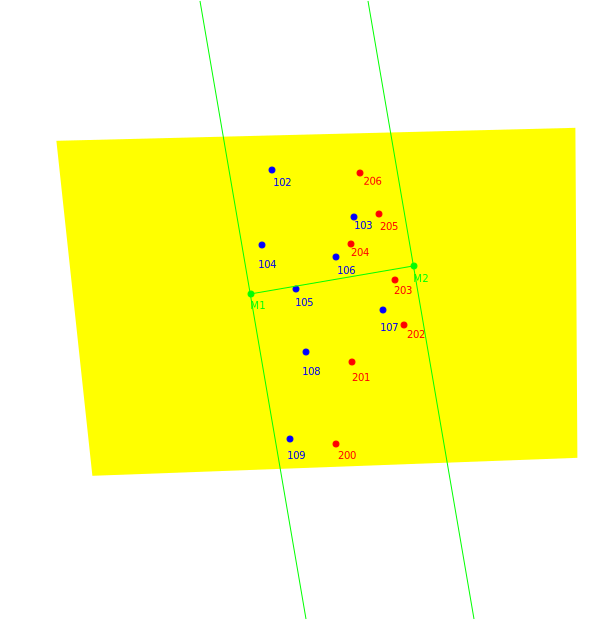
\includegraphics[scale=0.6]{RectDist.eps}
	\caption[Punkte mit einem rechtwinkeligen Abstand zur Schwerpunktlinie]{Alle Punkte von $B_1$ und $B_2$, die in dem Streifen zwischen den beiden Schwerpunkten liegen.}
	\label{fig:RectDist}		
\end{figure}


Nun nimmt man aus jeder Liste die beiden oberen Punkte und betrachtet sich die Linie, die sich zwischen diesen Punkten aufspannt. Schneidet diese Linie keines der beiden Polygone (außer an den Endpunkten), so merkt man sich den Mittelpunkt der Linie in der Liste: $Mittelpunktlinie$. Aus den Listen wird nun der größere der beiden Punkte gelöscht, falls dieser nicht der letzte in der Punktliste ist. Dieses Vorgehen wird solage vortgesetzt, bis beide Listen nur noch ein einziges Element haben. Die fiktiven Verbindungslinien und ihre Mittelpunkte sind auf der Abbildung~\ref{fig:Mittelpunkte} zu sehen.

\begin{figure}
	\centering
	\includegraphics[scale=0.6]{Mittelpunkte.eps}
	\caption[Verbindungslinien und deren Mittelpunkte]{Alle gefilterten Punkte aus $B_1$ und $B_2$, die zulässigen Vergindungslinien und deren Mittelpunkte.}
	\label{fig:Mittelpunkte}
\end{figure}

Der Linienzug, der nun in der Liste $Mittelpunktlinie$ liegt, liegt genau zwischen den beiden Polygonen und bildet die Struktur der Polygone an der Stelle ab, wo die beiden Polygone einander zugewant sind. Dieser Linienzug ist unter Abbildung~\ref{fig:MittelpunktLinie} zu sehen.

\begin{figure}
	\centering
	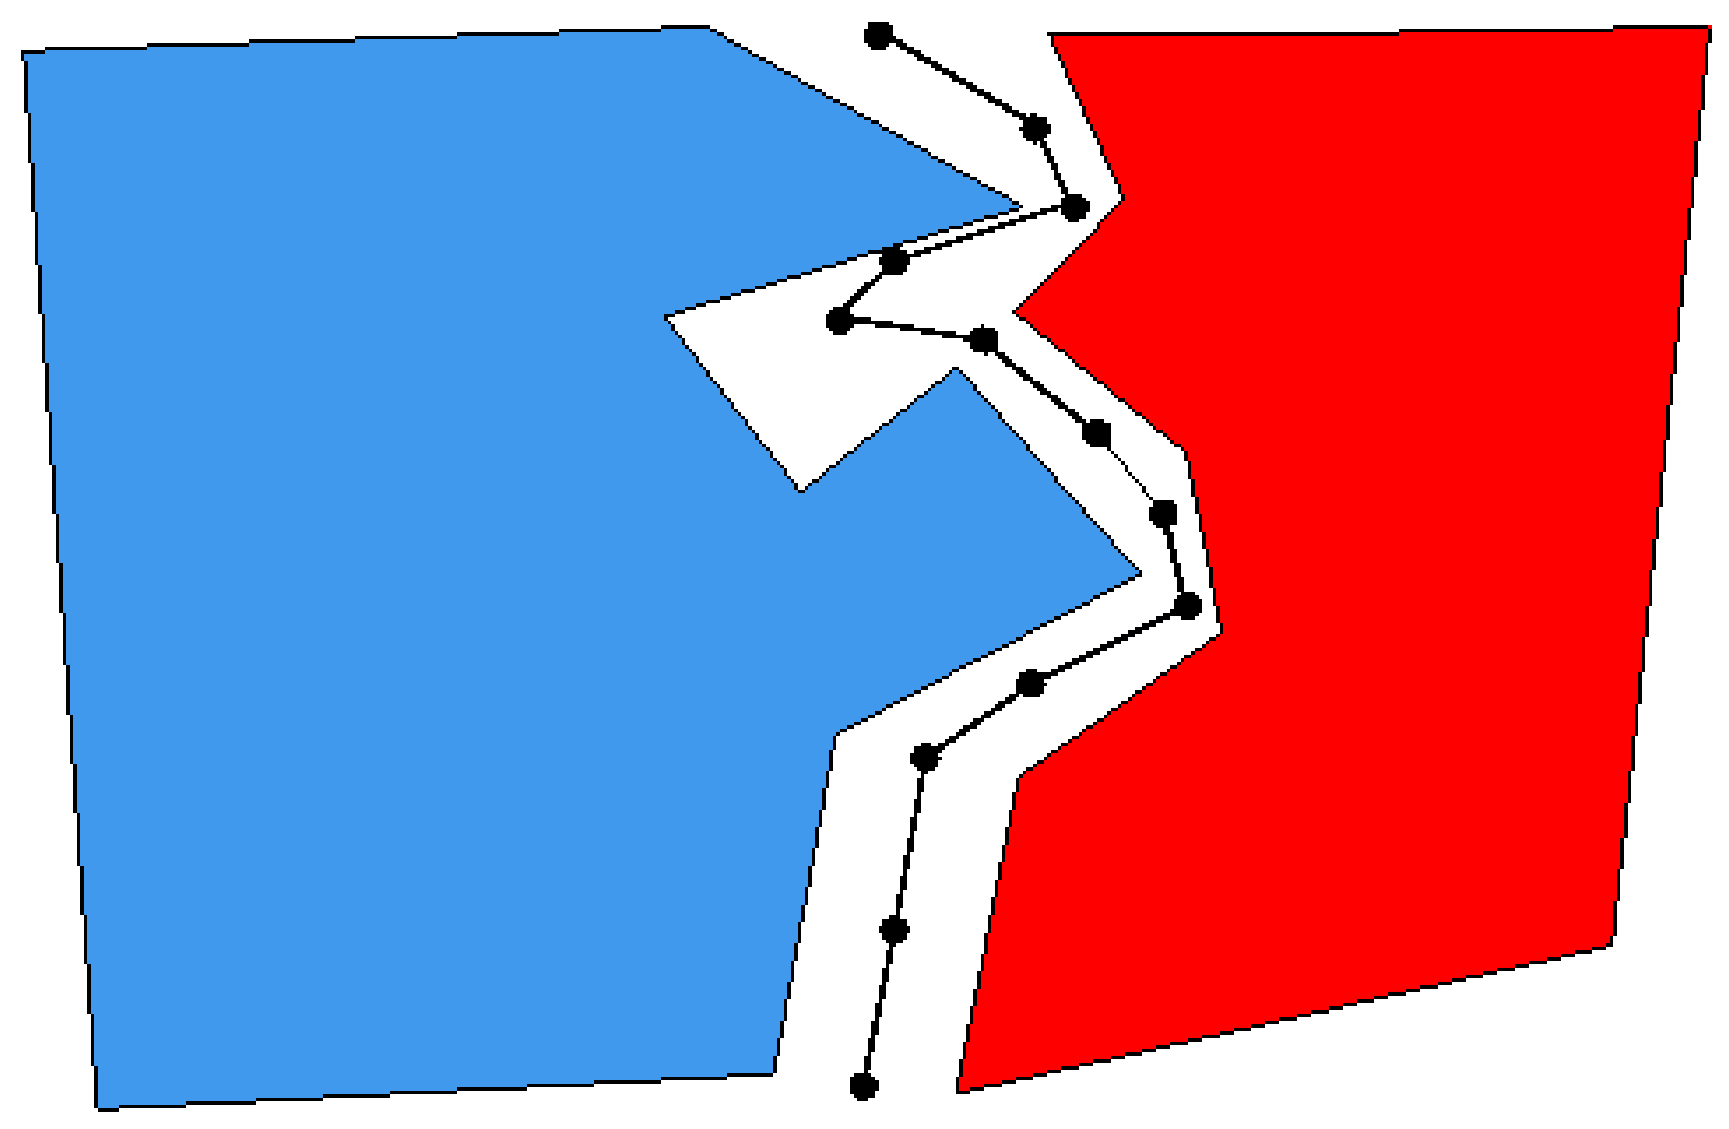
\includegraphics[scale=0.6]{MittelpunktLinie.eps}
	\caption{$B_1$ und $B_2$ mit dem berechneten Linienzug.}
	\label{fig:MittelpunktLinie}
\end{figure}

In der Regel teilt diese Linie  nun aber $A$ nicht, wie man an dem Beispiel gut sehen kann. Damit diese Linie nun wirklich duch $A$ geht, $A$ komplett geteilt wird und die Lage von $B_1$ und $B_2$ trotzdem noch wiedergespiegelt werden, führe ich folgende Schritte aus:

\begin{enumerate}
\item Berechne die Schwerpunkte $M_L$ der Linieneckpunkte, $M_A$ von $A$ und $M_B$ aller Eckpunkte von $B_1$ und $B_2$.
\item Berechne den Skallierungsfaktor $s_1=\frac{|A|}{|B_1|+|B_2|}$. 
\item Berechne das Maximum der Entfernungen von $M_L$ zu den beiden Endpunkten des Linienzuges, $d_L$ 
\item Berechne die maximale Entfernung von $M_A$ zu den Eckpunkten von $A$, $d_A$.
\item Berechne den Skallierungsfaktor $s_2=\frac{d_A}{d_l} * 1,05$. Die 5\% sind wilkürlich gewählt, und sollen die Warscheinlichkeit erhöhen, dass beide Endpunkte des neuen Linienzuges außerhalb von $A$ liegen. 5\% haben sich duchaus bewährt.
\item Berechne den neuen Linienzug $l'_1,l'_2,\hdots ,l'_n$ durch $l'_i=M_A+(l_i-M_l)*s_1+(M_l-M_B)*s_2$.
\end{enumerate}


Abbildung~\ref{fig:SplitLine} zeigt das Ergebniss an unserem Beispiel. 

Wie man schon an dem wilkürlichen Faktor 5\% sehen kann, liefert dieser Algorithmus bestimmt nicht in allen Fällen ein zulässiges Ergebnis. Die Erfolgsquote scheint aber sehr hoch zu liegen, in allen Beispielen, die ich beim Entwickeln durchgespielt habe tauchte kein einziger Fall auf, wo der Splitt versagte. Die Ergebnisse sahen auch alle sehr natürlich aus.


\begin{figure}
	\centering
	\includegraphics[scale=0.6]{Ergebnis.eps}
	\caption{Das Polygon $A$ mit der berechneten SplitLine.}
	\label{fig:SplitLine}
\end{figure}


\subsubsection{Zerteilete Löcher als Konkativitäten in ein Cycle einbauen}\label{JoinLL}

Wenn es bei der Teilung eines Faces dazu kommt, dass auch ein Hole geteilt wird, so werden aus den beiden neuen Polygonen Konkavitäten in den beiden neuen Faces. Zunächst muss jede dieser Konkativitäten dem passenden Face zugeordnet werden. Hierzu sucht man sich einfach einen Punkt des neuen Polygons der nicht auf dem Rand eines Faces liegt. Das passende Face ist dann dasjenige, in welchem der gewählte Punkt liegt. 

Als Beispiel betrachen wir das Polygon $A$ aus dem letzten Abschnitt als Face und ergänzen dieses durch ein Hole. Als Schnittlinie wird die eben berechnete benutzt. (siehe Abbildung~\ref{fig:JLL1})

\begin{figure}
	\centering
	\includegraphics[scale=0.6]{JLL1.svg.eps}
	\caption[EinFace mit einem Hole wird geteilt]{$A$ aus dem letzten Beispiel, jetzt um ein zu teilendes Hole ergäntzt.}
	\label{fig:JLL1}
\end{figure}

Der Algorithmus zum Vereinigen der Polygone bekommt nun also zwei Polygone, als geordnete Listen von Eckpunkten, das neue Face und ein passendes Bruckstück eines Holes. Diese Punktlisten werden zunächst sortiert. Die Punkte des Face werden wie gewöhnlich gegen den Uhrzeigersinn  angeordnet, die des Holes hingegen im Uhrzeigersinn. Zunächst suchen wir einen Punkt auf dem Rand des Faces, der nicht auf dem gemeinsamen Rand von Hole und Face liegt. Im Beispiel wählen wir Punkt 0.

Jetzt gehen wir die Punkte des Faces durch, solange auf der Linie zwischen dem aktuellen Punkt und dem Nächsten kein Punkt des Holes liegt. Alldiese Punkte fügen wir der Ergebnissliste $res$ hinzu.

Also: $rs=(0, 1, 2, 3, 4, 5)$.

Dann suchen wir aus allen Punkten des Holes, die auf der Linie von 5 zu 6 liegen, den Punkt der am nächstn zu 5 liegt. In unserem Fall ist das 107, den wir wieder an $res$ anhängen. Dieses etwas kompliziert klingende Vorgehen deckt eine Reihe von Sonderfällen ab, die hier auftauchen können. Abbildung~\ref{fig:SonderfaelleJLL} zeigt diese exemplarisch.

$res=(0, 1, 2, 3, 4, 5, 107)$

Nun durchlaufen wir die Punkte des Holes, beginnend mit 100, solange, bis der aktuelle Punkt auf dem Rand des Faces liegt (hier 103). Alle besuchten Punkte werden an $res$ angehängt.

Daraus folgt: $res=(0, 1, 2, 3, 4, 5, 107, 100, 101, 102, 103)$

Anschließend durchlaufen wir wieder das Face, wobei wir bei 6 beginnen, und suchen den ersten Punkt, der nicht auf dem Hole liegt. Im Beispiel ist dies Punkt 9.

Abschließend hängen wir an $res$ alle Punkte an, bis wir wieder am Ausgangspunkt angelangt sind.

Schließlich ist $res=(0, 1, 2, 3, 4, 5, 107, 100, 101, 102, 103, 9, 10, 11, 12)$. Abbildung~\ref{fig:JLL3} zeigt das Ergebniss als Polygon.


\begin{figure}
	\centering
	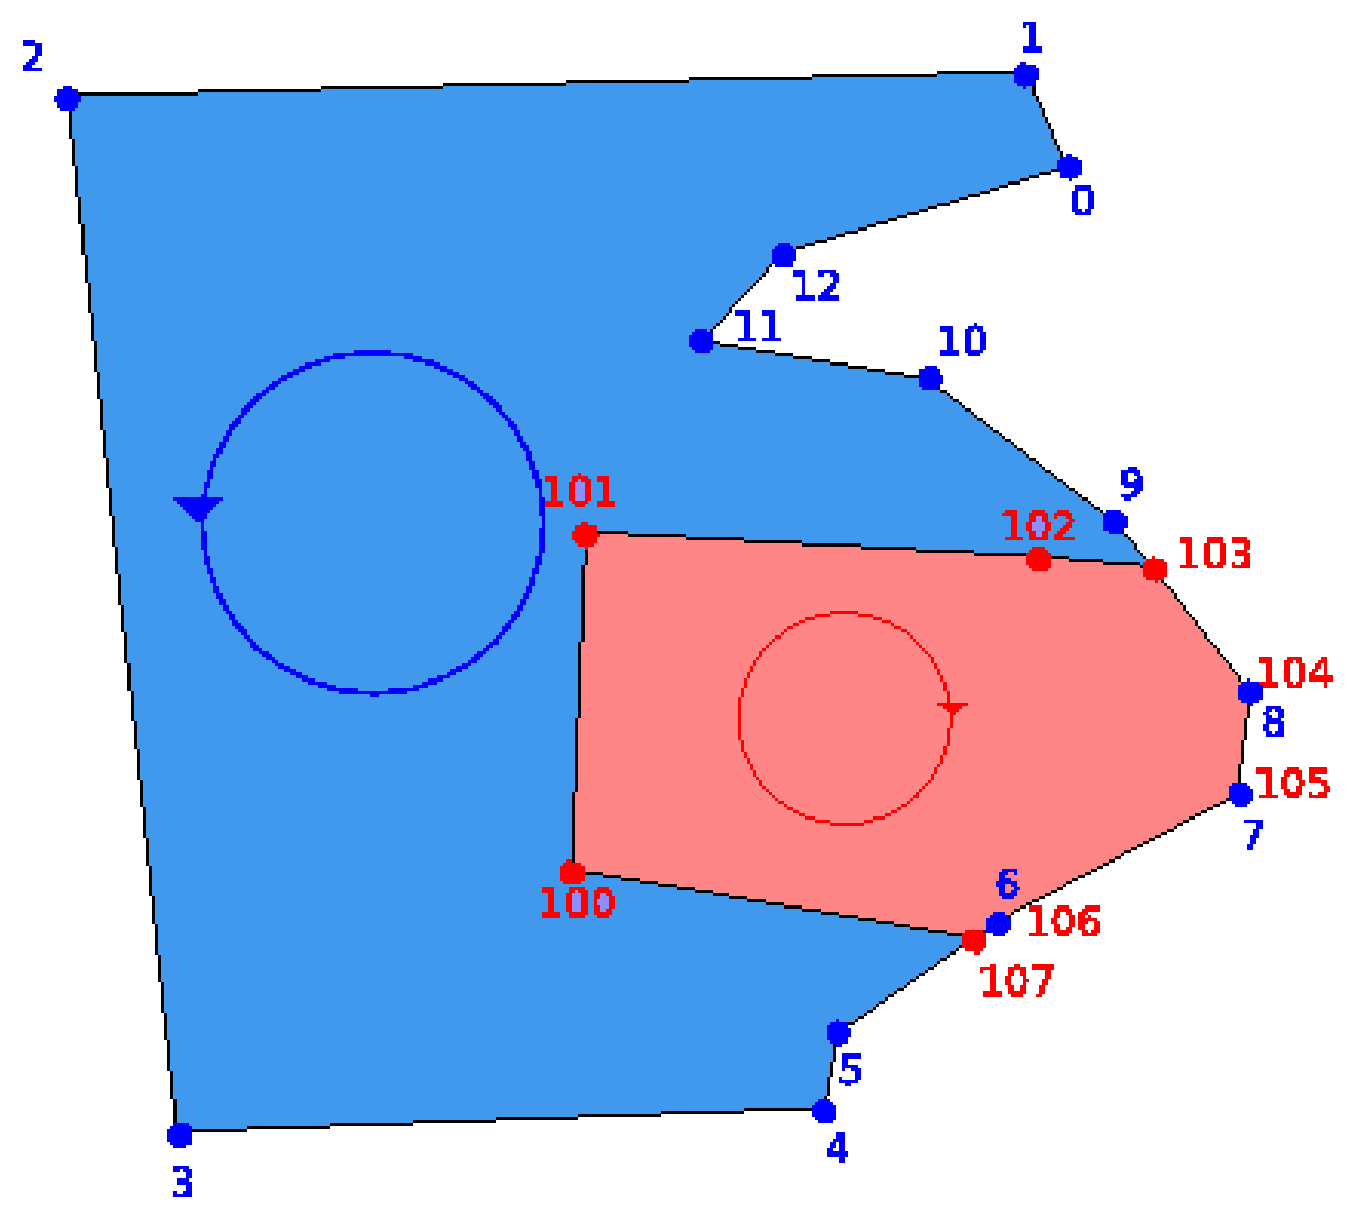
\includegraphics[scale=0.6]{JLL2.svg.eps}
	\caption{Die beiden neuentstandenen Polygone sollen verbunden werden.}
	\label{fig:JLL2}
\end{figure}


\begin{figure}
\subfigure[Beide Berührungspunkte liegen auf der selben Facelinie.]{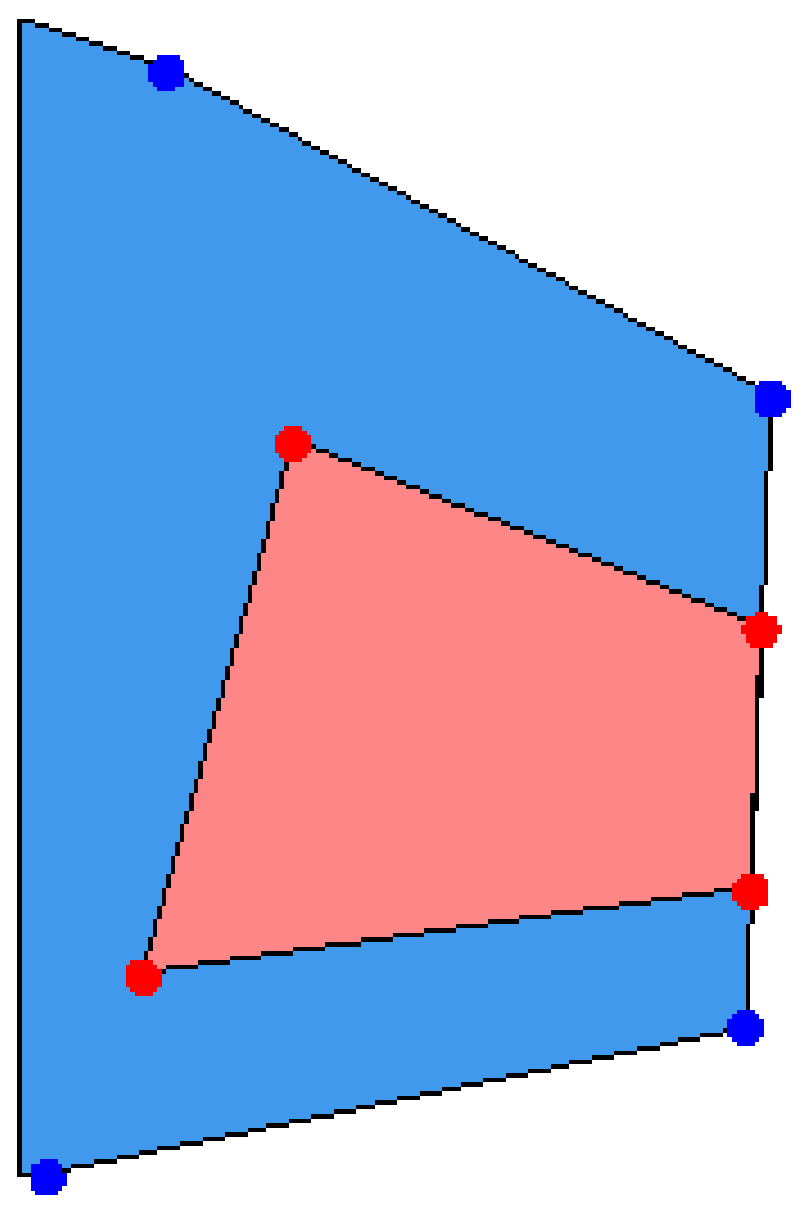
\includegraphics[width=0.35\textwidth]{Sonderfall1JLL.svg.eps}}\hfill
\subfigure[Der erste Punkt des Holes ist auch ein Punkt des Faces]{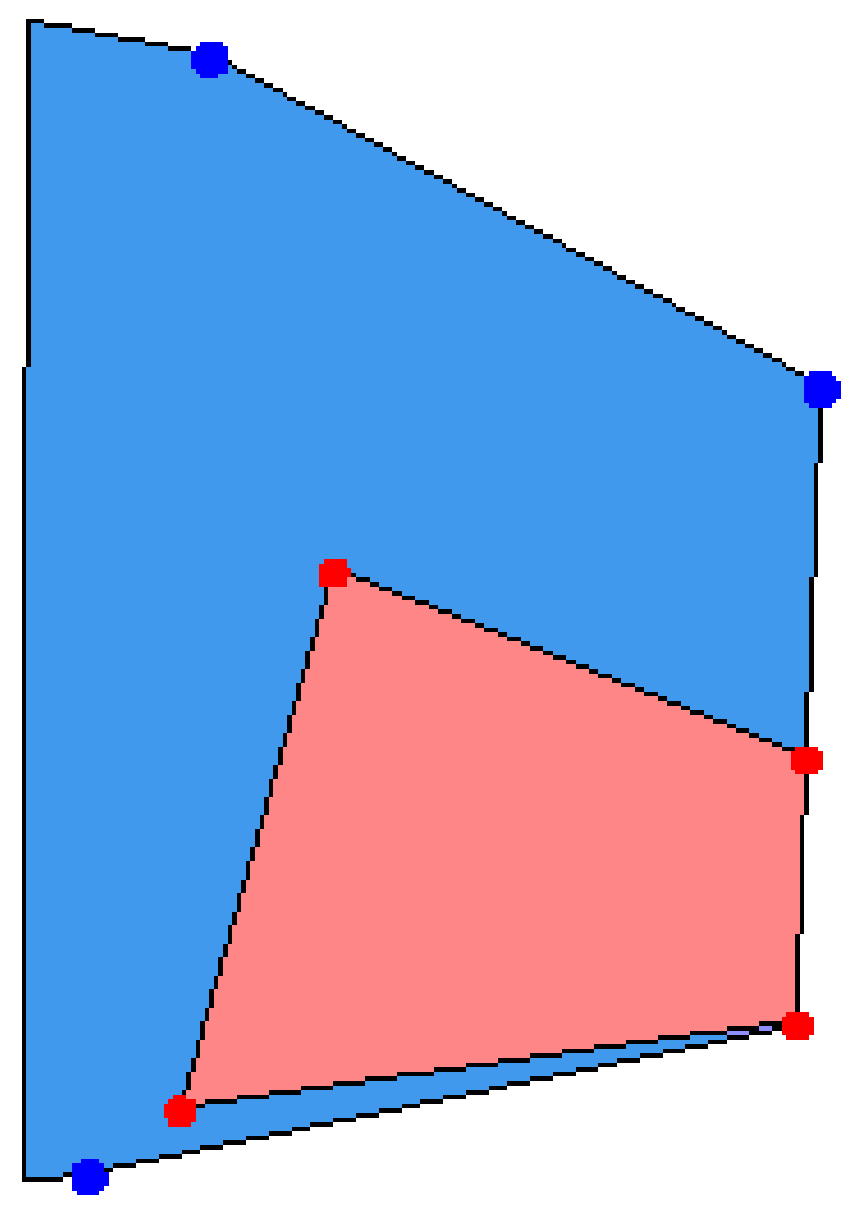
\includegraphics[width=0.35\textwidth]{Sonderfall2JLL.svg.eps}}
\caption[Sonderfälle, die bei der Vereinigung auftreten können]{Sonderfälle, die bei der Vereinigung auftreten können und wegen denen man die Funktion $getClosestBoundaryPoint$ benötigt.}
\label{fig:SonderfaelleJLL}
\end{figure}



\begin{figure}
	\centering
	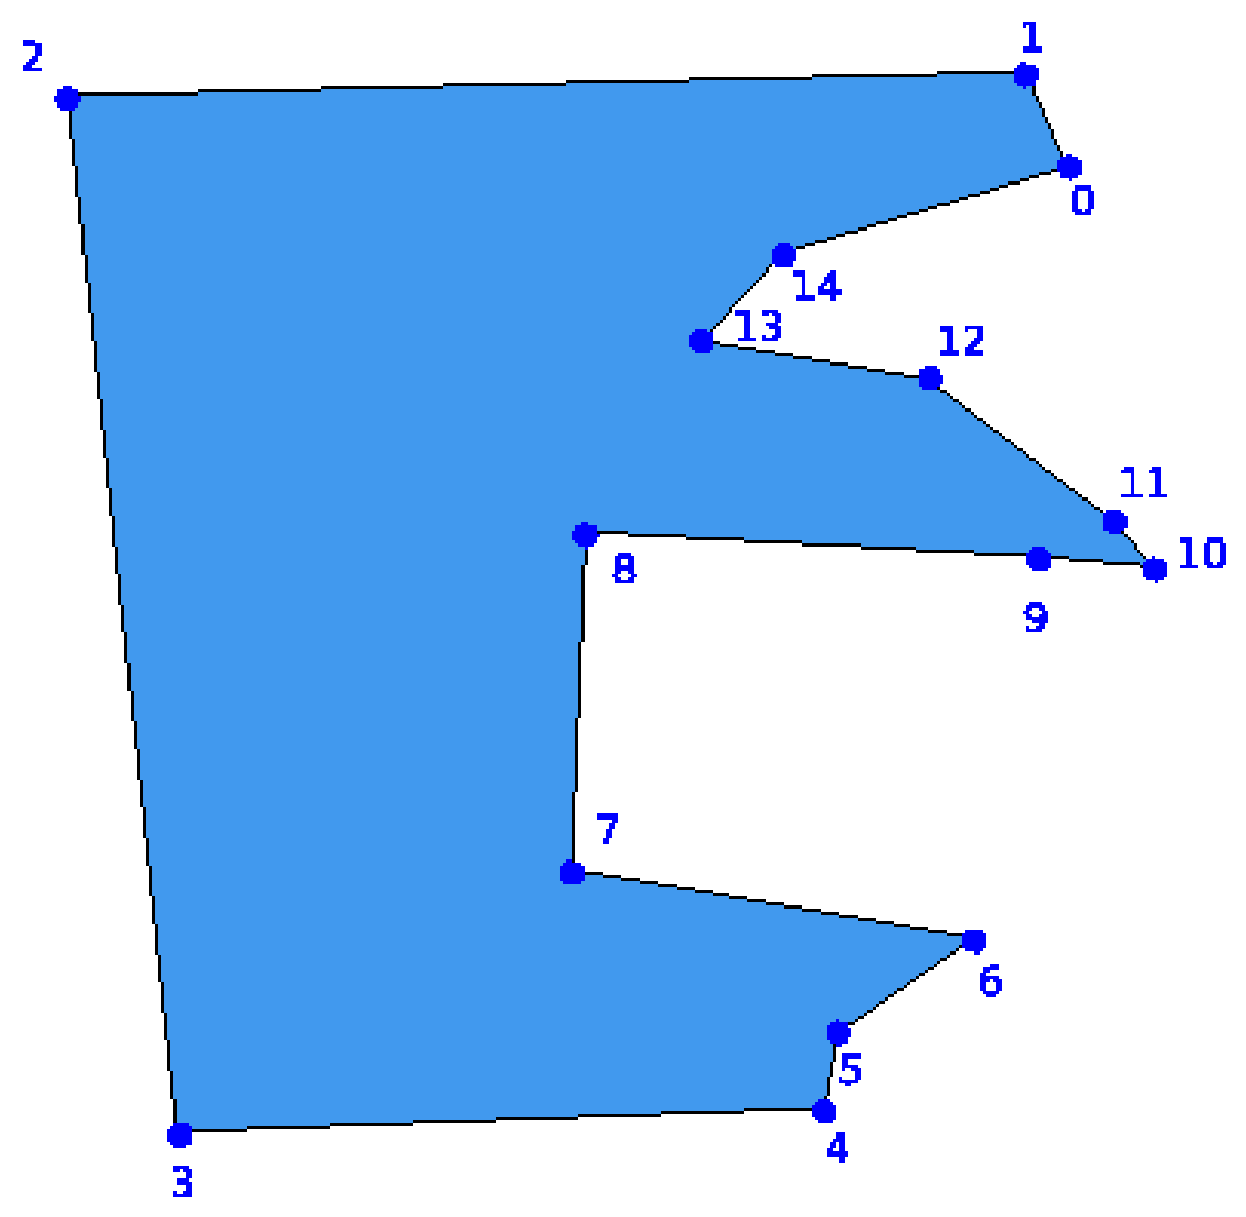
\includegraphics[scale=0.6]{JLL3.svg.eps}
	\caption{Das fertig zusammengesetzte Polygon.}
	\label{fig:JLL3}
\end{figure}



\subsubsection{\index{Rotaring Pane}Rotaring Pane} \label{rotPane}
In \cite{TG} wurde bereits der Algorithmus ,,rotating Pane'' vorgestellt. I, Laufe meiner Arbeit musste ich diesen Algorithmus nachprogrammieren, und habe hierbei eine Version gefunden, die etwas einfacher ist und erheblich weniger Fallunterscheidungen benutzen muss.

Die Idee dieses Algorithmusses ist es zu jeder Kante den Winkel zu bestimmen, den dieser mit der x"~Achse einnimmt. Zu zwei Ecken, die eine gemeinsame Kante bilden konstruiert man ein Dreieck mit dem Startpunkt der Kante des anderen Polygones zu bilden, dessen Winkel zwischen den Winkeln des Startpolygones liegt.

\begin{figure}
	\centering
	
\includegraphics{feu_logo2.eps}
	\caption[Tabellendarstellung des ,,rotating Pane'']{Diese Abbildung zeigt die beiden Felder zweier Vierecke und zeigt, welche Punkte zusammen ein movingsegment bilden.}
	\label{fig:RotatinPane}
\end{figure}


Hierzu werden zwei Felder von Punkten gebildet, für jeder Polygon eines. Zu Punkt jedem Punkt wird dann der Winkel hinzugefügt, den die Linie hat, welche von diesem Punkt ausgeht. Die Felder werden dann nach diesen Winkel sortiert. Zu zwei aufeinanderfolgenden Punkten der ersten Polygones wird dann der passende Punkt aus dem anderen Polygon gesucht. Hierzu wird die Funktion ,,finde\_passenden\_Index'' benutzt, die weiter unten erklärt wird. Das so entstandene Dreieck (als movingsegment) wird dann der Rückgabestruktur hinzugefügt.

\begin{algorithm}[!ht]
		\SetKwFunction{fMI}{finde\_passenden\_Index}
	\caption{Rotaring Pane Allgorithmus, um aus zwei konvexen H"ullen moving segments zu erstellen}
	\Ein{KH"ulle1 und KH"ulle2, zwei konvexe H"ullenb"aume}
	\Ergebnis{Eine Menge von moving segments, die die Interpolation der beiden Polygone darstellt}
	\Begin{
		Bestimme $KH1$ und $KH2$ die konvexen H"ullen der Polygone als Feld von LineWAs\;
		Berechne die Winkel in jedem Eckpunkt von $KH1$ und $KH2$\;
		Sortiere $KH1$ und $KH2$ aufsteigend nach diesen Winkeln\;
		$j:=0$\;
		\Fuer{$i<KH1.l"ange$}{
			$j:=\fMI{KH2, j, KH1[i].winkel, \text{false}}$\;
			F"uge das moving segment:$(KH1[i],KH1[i+1],KH2[j]$ dem Ergebnis-Feld hinzu\;
}			
		$j:=0$\;
		\Fuer{$i<KH2.l"ange$}{
			$j:=\fMI{KH1, j, KH2[i].winkel,\text{true}}$\;
			F"uge das moving segment:$(KH2[i],KH2[i+1],KH[j]$ dem Ergebnis-Feld hinzu\;
}			
}
\end{algorithm}


Diese Funktion durchsucht ein Feld, dass ein konvexes Polygon in der Form wie oben darstellt, nach dem übergebenen Winkel. Die Suche startet bei dem Index ,,Startindex''. Je nach dem Wert des Winkels an der angegebenen Stelle wird nach linkls oder rechts rekursiv weitergeangen. Sollten zwei Winkel exakt gleich sein, die Kanten also parallel sein, so muss man das Ergebniss unterschiedlich behandeln. Dieses leistet der Wert ,,Gleiche\_Winkel''.

\begin{function}[!ht]
	\caption{finde\_passenden\_Index(Polygon, Startindex, Winkel, Gleiche\_Winkel)}
	
	\Ein{\begin{tabular}{ll}
		Polygon: &Das zu durchsuchende konvexe Polygon als Feld\\
 			&von LineWAs\\
		Startindex: &Der Index, an dem die Suche beginnen\\
 				&soll\\
		Winkel: &Der Winkel, zu dem der passende Index gesucht\\
 			&wird\\
		Gleiche\_Winkel: &Dieser boolsche Parameter gibt an, \\
				&wie mit parallelen Kanten verfahren werden soll
	     \end{tabular}
}
	\BlankLine
	\Ergebnis{Der Index des Punktes, an dem die Linie anf"angt, mit der die Ecke mit dem "ubergebenen Winkel gematched wird}
	\Begin{	
        	\uWenn {$Winkel<Polygon[0].Winkel$}	{
        		Gebe den Index 0 zur"uck\;
}
        	\uWenn{$Polygon[0].Winkel=Winkel$ und $Gleiche\_Winkel$}{
        			Gebe den Index 0 zur"uck\;
}        
        	\Wenn{$Winkel>Polygon[letzer\_Index].Winkel$}{
        		Gebe den Index 0 zur"uck\;
}
	
        	\Solange{Nicht $(Polygon[j].Winkel\geq Winkel$ und $Polygon[j-1].Winkel\leq Winkel)$}{
        		\uWenn{$(j\neq0$ und $Winkel<Polygon[j-1].Winkel$}{
        			$j:=j-1$\;
}	
 	           	\Sonst{
				\Wenn{$Polygon[0].Winkel\neq Winkel$}{
		                 	$j:=j+1$\;
}
}
}
		\Wenn{$Polygon[j].Winkel=Winkel$ und $Gleiche\_Winkel$}{
	        	$j:=j+1$\;
}
		Gebe den Index $j$ zur"uck\;
}		
\end{function}

\clearpage

\subsubsection{Zerlegung von einfachen Polygonen in konvexe Polygone}\label{Zerlegung}

Um beliebige Polygone in VRML-Dateien exportieren zu können, musste ich einen Algorithmus finden, der beliebige, einfache Polygone in konvexe zerlegen kann. Natürlich hätte ich einfach eine Dreieckszerlegung vornehmen können, diese Zerlegung wäre aber möglicherweise erheblich kleinteiliger, als ich das eigentlich brauchte. Die Idee des Algorithmusses ist auch ganz einfach:

Ecken, deren Wickel größer als 180\degree\/ sind, so genannte konvexe Ecken, stören und müssen beseitigt werden. Teile ich ein Polygon an einem Winkel, so wird dieser kleiner. Also kann man Polygon solage, an konvexen Ecken,  zerteilen, bis es in keinem der Ergebnisspolygone noch einen konvexen Winkel gibt.

Teilen kann man ein Polygon an zwei Ecken $A$ und $B$, falls die Verbindung von $A$ und $B$ innerhalb des Polygones liegt, und keine unbeteiligte Kante geschnitten wird.

Verbessen kann man diesen Ansatz noch dardurch, dass man zuerst versucht das Polygon an zwei konvexen Ecken zu teilen.

Dieser Algorithmus funktioniert nicht nur für einfache Polygone, sondern auch für solche, in denen eine Kante zweifach durchlaufen wird. Damit kann man auch Faces mit Holes zerlegen.

\begin{figure}
	\centering
	
\includegraphics{feu_logo2.eps}
	\caption{Ein Beispiel, wie ein Face mit einem Hole in konvexe Polygone zerfällt.}
	\label{fig:ZerlegungFace}
\end{figure}


\begin{algorithm} [!ht]
	\SetKwFunction{gCV}{liefere\_konvexe\_Ecken}
	\SetKwFunction{iSA}{ist\_teilbar}
	\caption{Zerlegung von einfachen Polygonen in konvexe Polygone}
	\Ein{Eine Menge $Polygone$ von einfachen Polygonen, repr"asentiert durch geordnete Punktlisten}
	\Ergebnis{Die Menge $Polygone$ besteht nur noch aus konvexen Polygonen}
	\Begin{
		$aktuell:=0$\;
		$konvexe\_Ecken=\emptyset$\;
		\Wiederh{$|konvexe\_Ecken|=0$ und $aktuell=|Polygone|$}{
            		$aktuelles\_Polygon=Polygone[aktuell]$\;
			$konvexe\_Ecken=aktuelles\_Polygon.\gCV{}$\;
			\uWenn{$|konvexe\_Ecken|>0$}{
				\Wenn{$|konvexe\_Ecken|>1$}{
					\Fuer{$i<|konvexe\_Ecken|$}{
						\Fuer{$j:=i+1$ \KwTo $j<|konvexe\_Ecken|$}{
							\Wenn{$aktuelles\_Polygon.\iSA{konv\_Eck[i],konv\_Eck[j]}$}{
								Teile $aktuelles\_Polygon$ an den Ecken $konvexe\_Ecken[i]$ und $konvexe\_Ecken[j]$\;
								Ersetzt $aktuelles\_Polygon$ in $Polygone$ durch die beiden neuen Polygone\;
								Durchlaufe alle Scheifen von neuem\;
}
}
}
}
                		$Index1:=konvexe\_Ecken[0]$\;
				$Index2:=Index1+\frac{|aktuelles\_Polygon|}{2}$\;
				\Fuer{$i<|aktuelles\_Polygon|$}{
					$split\_Index=Index2+\frac{(-1)^i i}{2}$\;
		                    	\Wenn{$aktuelles\_Polygon.\iSA{Index1,split\_Index}$}{
		                    	Teile $aktuelles\_Polygon$ an den Ecken $Index1$ und $split\_Index$\;
								Ersetzt $aktuelles\_Polygon$ in $Polygone$ durch die beiden neuen Polygone\;
}
}
}
			\Sonst{
				$aktuell:=aktuell+1$\;
}

}
}
\end{algorithm}

\clearpage

\subsubsection{\index{ConvexHullTreeNode!Konstruktion}Aufbau eines ConvexHullTrees}\label{constCHTN}
Der Algorithmus zum Aufbau eines ConvexHullTrees wurde in \cite{TG} bereits erl"autert. Da dieser aber von zentraler Bedeutung zur L"osung des Problems ist, bespreche ich den Algorithmus an dieser Stelle noch einmal.

Als Beispiel dient mir ein Polygon aus der GERMANY-Datenbank. Bei diesem Polygon handelt es sich um die Gemeinde Sandershausen, die als Enklave zu dem Stadtkreis Kassel geh"ort. Abbildung~\ref{fig:Sanders} zeigt dieses Polygon in dem dazugeh"origen Luftbild, dass ich aus der Applikation Google-Earth entnommen habe. 

Der erste Schritt, bei der Erzeugung eines ConvexHullTree-Kontens, ist die Ereugung der konvexen H"ulle des Polygons. In den Abbildungen~\ref{fig:sand2} ist diese in Rotbraun eingezeichnet. Der Allgorithmus, der zur Erzeugung der H"ulle benutzt wird ist der \index{Graham Scan}Graham Scan Algorithmus, der zu den Standard-Allgorithem zu z"ahlen ist. In \cite{G72} wurde dieser Algorithmus das erste Mal beschrieben. Eine gute Beschreibung finden Sie \anmerkung{hier Literaturstelle einf"ugen}.

Im Anschu"s daran wird das Ausgangspolygon nach zusammenh"angenden Linienz"ugen durchsucht, die nicht in der konvexen H"ulle enthalten sind. Diese Suche wird mittels eines parallelen Durchlaufs duch beide Linienz"uge realisiert.

Schlie"slich wird diser Algorithmus rekursiv f"ur alle diese Linienz"uge aufgerufen und die Ergebnisse werden an die entsprechenden Stellen in den Vaterknoten eingeh"angt.

\begin{figure}
	\centering
	\includegraphics[width=10cm]{Sandershausen.eps}
	\caption{Die Gemeinde Sandershausen als Beispiel eines ConvexHullTrees}
	\label{fig:Sanders}
\end{figure}
\begin{figure}
\subfigure[die Nodes der Level 0-1]{\includegraphics[width=0.45\textwidth]{Sandershausen2.eps}}\hfill
\subfigure[kompletter ConvexHullTree]{\includegraphics[width=0.45\textwidth]{Sandershausen3.eps}}
\caption{Ausschnitt von Sandershausen mit verschieden detailierten ConvexHullTrees}
\label{fig:sand2}
\end{figure}
%\begin{figure}%
	%\centering
	%\includegraphics[width=5cm]{Sandershausen2.eps}
	%\caption{Ausschnitt von Sandershausen mit den Nodes der Level 0-1}
	%\label{fig:sand2}
%\end{figure}
%\begin{figure}
%	\centering%
	%\includegraphics[width=5cm]{Sandershausen3.eps}
	%\caption{Ausschnitt von Sandershausen mit dem kompletten ConvexHullTree}
	%\label{fig:sanders3}
%\end{figure}

\begin{algorithm}[!ht]

\SetKwFunction{cH}{berechne\_konvexe\_H"ulle}
	\caption{Erzeuge einen konvexen H"ullenbaum aus einem Polygon}
	\Ein{\begin{tabular}{ll}
		Polygon: &Ein Polygon,rep"asentiert duch eine geordnete Liste von \\
			&Eckpunkten\\
		Ebene:	&Die Ebene des zu Erzeugenden Elementes\\
		ist\_Loch: &Ein boolscher Parameter der angibt, ob das neue Element \\
			&zu einem Loch geh"ort\\
		Vater:	&Das Vaterelement des Neuen\\
		\end{tabular}
}
	\BlankLine
	\Ergebnis{Ein konvexer H"ullenbaum, der das "ubergebene Poygon beschreibt}
	\Begin{
	
%         LineWA[] tmplist, convhull, childlist;
	Setze die Klassen-Variabeleln $ist\_Loch$ und $Vater$\;

%         int node;
%         int index1, index2, length, lastindex, noiterations;
%         int indexll1, indexll2;
%         this.linelist = new Vector();
%         smallesty = Integer.MAX_VALUE;
%         smallestx = Integer.MAX_VALUE;
%         smallestpoint = -1;       
	$konvexeH"ulle:=\cH(Polygon)$\;
%         // Find where the first node in linelist is in the convex hull
%         // (Or the earliest possible if the first node is not on the hull)
%         // This is to preserve the order in the linelist in the ordering of
%         // points in the convex hull tree node.
	$startindex:=0$\;
	$endindex:=konvexeH"ulle.L"ange$\;
	Finde den Index, in der konvexen H"ulle, der dem niedrigsten Index in dem Polygon entspricht, und speichere Ihn in $startindex$\;
	Finde den Index, in der konvexen H"ulle, der dem h"ochsten Index in dem Polygon entspricht, und speichere Ihn in $endindex$\;
         %for (int a=0;a<linelist.length;a++)
% {
%             index1 = TriRepUtil.indexOf(convhull, linelist[a]);
%             if (index1 != -1) break;
% }
%         for (int a=linelist.length-1;a>=0;a--)
% {
%             lastindex = TriRepUtil.indexOf(convhull, linelist[a]);
%             if (lastindex != -1) break;
% }
	\uWenn{$startindex<endindex$}{
		\Fuer{$i:=startindex$ \KwTo $i\leq endindex$}{	
			Speichere $konvexeH"ulle[i]$ in der linelist des neuen Konten\;
}
}
	\Sonst{
		
        	\Fuer{$i:=index1$ \KwTo $konvexeH"ulle.L"ange$}
{
			Speichere $konvexeH"ulle[i]$ in der linelist des neuen Konten\;
}
		\Fuer{$i:=0$ \KwTo $endindex$}
{
			Speichere $konvexeH"ulle[i]$ in der linelist des neuen Konten\;
}
}
%         // Check lines in convex hull with lines in line list. Whenever two points
%         // which are neighbours in the convex hull are not neighbours in the line
%         // list, create a child node from the points between them.
%         
%         noiterations = numberOfLines();
%         index1 = 0;
%         indexll1 = 0;
%         while (!(linelist[indexll1].equals(getLine(index1))))
% {
%             indexll1++;
% }
	\Fuer{$i<konvexeH"ulle.L"ange$}
{
%             index2 = index1+1;
%             indexll2 = indexll1+1;
%             while (!(linelist[indexll2 % linelist.length].equals(getLine(index2 % noiterations))))
% {
%                 indexll2++;
% }
%             
%             if ((indexll2 != indexll1+1) && ((level == 0) ||
%                     ((indexll2 != linelist.length) && (indexll1 != linelist.length-1)))
%                     && (indexll2 != indexll1-1))
% {
%                 // create child node
%                 length = indexll2-indexll1+1;
%                 childlist = new LineWA[length];
%                 for (int b=0;b<length;b++)
% {
%                     if ((b+indexll1) < linelist.length)
% {
%                         childlist[length-b-1] = linelist[b+indexll1];
% }
%                     else
% {
%                         childlist[length-b-1] = linelist[b+indexll1-linelist.length];
% }
% }
%                 insertChild(index1, new ConvexHullTreeNode(childlist, level+1,this.isHole,this));
% }
%             index1 = index2;
%             indexll1 = indexll2;
}
}
 \end{algorithm}

\clearpage
\subsubsection{Bestimmung der maximalen Distanz mehrerer Polygone}\label{maxDist}
\label{gmD}
Die Berechnung der größten Abstandes den zwei Punkte aus verschiedenen Polygonen ist eine relativ aufwendige Operation, mit quadratischem Aufwand. Dieser Algorithmus liefert einen sehr ähnlichen Wert in $O(n\log(n))$. Dieser Wert ist der Durchmesser der konvexen Hülle der Punkte beider Polygone. 

Zur Berechnung dieses Wertes wird zuerst die gemeinsame konvexe Hülle der beiden Polygone berechnet. Dann wird von jedem Punkt der konvexen Hülle die maximale quadratische Distanz berechnet und die Wurzel der größten Distanz zurückgegeben.

\begin{algorithm}[!ht]
	\SetKwFunction{gLDFP}{l"angste\_Entfernung\_von\_Punkt}
	\SetKwFunction{dist}{Quadrat\_der\_Entfernung}
	\caption{Bestimmung der maximalen Distanz mehrerer Polygone}
	\Ein{Mehrere Polygone repr"asentiert duch ihre Punktlisten}
	\Aus{Der maximale Abstand von zwei Punkten}
	\Begin{
		Bilde eine gemeinsame Punktliste durch konkatenieren der Eingangslisten\;
		Bilde $CH$ die konvexe H"ulle der Eingangsdaten\;
		$i:=0$\; 
		$tmpdist:=0$\;
		$pos:=\frac{CH.length}{2}$\;
		\Fuer{$i<CH.length$}{
			$pos:=\gLDFP{CH[i],CH,pos}$\;
			$distxy:=\dist{CH[i],CH[pos]}$\;
		        \Wenn{$distxy>tmpdist$}
{			
			           $tmpdist:=distxy$\;
}			
}    
		Das Ergebnis ist $\sqrt{tmpdist}$\;
}
\end{algorithm}
\clearpage

Diese Funktion sucht in einem konvexen Polygon den Punkt, der am weitesten von dem übergebenen Punkt entfernt ist. Der Punkt an dem Index Startindex ist der Punkt, mit dem zuerst verglichen wird. Die Suche läuft danach rekursiv weiter. 

\begin{function}[!ht]
	\SetKwFunction{dist}{Quadrat\_der\_Entfernung}
	\SetKwFunction{gLDFP}{l"angste\_Entfernung\_von\_Punkt}
	\caption{l"angste\_Entfernung\_von\_Punkt(Punkt, Polygon, Startindex)}
	\Ein{\begin{tabular}{ll}
Punkt: &Der Punkt, zu dem der Abstand gemessen wird,\\
	     Polygon: &Das konvexe Polygon, in dem der am weitesten \\
			&entfernte Punkt gesucht wird\\
	
	     Startindex: &Der Index an dem die Suche begonnen wird\end{tabular}}
	\BlankLine
	\Ergebnis{Der Index des Polygonpunktes, der von dem Punkt den maximalen Abstand hat.}
	\Begin{
		$distpos:=\dist{Punkt,Polygon[pos]}$\;
		$distposlinks:=\dist{Punkt,Polygon[pos+1]}$\;
		$distposrechts:=\dist{Punkt,Polygon[pos-1]}$\;
		\uWenn{$distpos\geq distposlinks$ und $distpos\geq distposrechts$}{
			Gebe $pos$ als Ergebnis zur"uck\;
}
		\Sonst{
			\uWenn{$distposlinks>distpos$}{
				Gebe $\gLDFP{Punkt, Polygon, (pos+1)}$ zur"uck\;
}		
			\Sonst{Gebe $\gLDFP{Punkt, Polygon, (pos-1)}$ zur"uck\;}
}
}
\end{function}

\label{getdist}
Diese Funktion liefert den Wert der quadratischen Entfernung von zwei Punkten zurück. Die Berechnung erfolgt nummerisch stabiler als die einfache Formel $(x_2-x_1)^2+(y_2-y_1)^2$. Besonders im Umgang mit geografischen Koordinaten ist dies wichtig.

\begin{function}[!ht]
	\caption{Quadrat\_der\_Entfernung(Punkt1, Punkt2)}
	\Ein{Die beiden Punkte, deren Abstand berechnet werden soll}
	\Ergebnis{Das Quadrat des Abstandes der beiden Punkte}
	\Begin{
		Berechne $x_1^2$ $x_2^2$, $y_1^2$, $y_2^2$, $x_1x_2$ und $y_1y_2$ in doppelter Genauigkeit\;
		Gebe $x_1^2+x_2^2+y_1^2+y_2^2-2(x_1x_2+y_1y_2)$ in einfacher Genauigkeit zur"uck\;
}
\end{function}


\clearpage
\subsection{Beschreibung der Klassen}\label{klassen}

\subsubsection{\index{LineWA}LineWA}

Diese Klasse repräsentiert einen zweidimensionalen Punkt, der durch eine Winkelangabe ergäntzt ist. Somit kann man ein Polygon speichern indem man alle seine Punkte speichert, und zu jedem Punkt noch den Winkel, den die Kante, die von dem Punkt ausgeht, mit der x"~Achse hat. Die Klasse ist so implementiert, dass mehrere LineWAs automatisch aufsteigen nach ihren Winkeln sortiert werden können.

\subsubsection{\index{CHLine}CHLine}

Die CHLine ist eine LineWA in einem ConvexHullTreeNode. Zusätzlich zu den bekannten Attributen kann diese auch noch einen ConvexHullTreeNode als Kind enthalten. Diese Klasse trägt quasi die rekursive Struktur des ConvexHullTrees.

\subsubsection{\index{LineDist}LineDist}

Diese Klasse dient dazu, Kombinationen von Punkten und Entfernungen speichern zu können. Wie bei der LineWA ist die Sortierung nach Entfernung möglich.

\subsubsection{\index{PointWNL}PointWNL}

Diese Klasse dient dazu Punkte im dreidimensionalen darstellen zu können.

\subsubsection{\index{ConvexHullTreeNode}ConvexHullTreeNode}

Diese Klasse repräsentiert den ,,konvexen Hüllenbaum'', der bereits öfter erwähnt wurde. Der ConvexHullTreeNode enthält an Attributen:

\begin{itemize}
\item linelist

Die linelist ist ein Feld von CHLines, enthält also alle Punkte der konvexen Hülle und die dazugehörigen Kinder.

\item level

Hiermit kann man feststellen, in welcher Tiefe sich ein ConvexHullTreeNode in dem ConvexHullTree befindet.

\item hole

Dieses boolsche Attribut legt fest, ob das Objekt zu einem Cycle,oder zu einem hole gehört.

\item myParent

Dieses Attribut zeigt auf das Vaterelement des Objektes in dem RegionTree. Der Vater kann entweder ein face, oder ein anderer ConvexHullTreeNode sein.

\end{itemize}

Die wichtigsten, nicht trivialen Methoden dieser Klasse sind:

\begin{itemize}
\item Konstruktor

Der Konstruktor ist näher unter \ref{constCHTN} beschrieben.

\item getLines

diese Funktion liefert die Punkte des Polygons zurück, die dieser ConvexHullTree beschreibt.

\item getCenter

liefert den Schwerpunkt der konvexen Hülle.

\item getSteinerPoint

liefert den Steinerpunkt der konvexen Hülle.

\item getSplitLine

liefert einen Linienzug, an dem das Objekt geteilt werden kann. Die beiden übergebenen konvexen Hüllenbäume dienen hierbei als Anleitung. Der entsprechende Algorithmus findet sich unter \ref{ZerteilungsAlgo}

\item getSplitNodes

diese Funktion teilt das Objekt an dem übergebenen Linienzug und liefert ein zweidimensionales Feld von Punkten zurück, die die beiden neuen ConvexHullTreeNodes repräsentieren.  

\end{itemize}


\subsubsection{\index{Face}Face}

Ein Face besteht aus einem Cycle und mehreren, oder keinem Hole. Sowohl der Cycle, als auch die Holes sind durch ConvexHullTrees gegeben. Die Attribute des Faces sind:

\begin{itemize}
\item Cycle

ein ConvexHullTreeNode, der das begrenzende Polygon dieses Faces beschreibt.

\item Holes

ein Feld von ConvexHullTreeNodes, das die Holes des Faces beinhalten.

\item parent

ein Verweis auf die Region (bzw. RegionForInterpolation), zu der dieses Face gehört.

\end{itemize}

Die wichtigsten, nicht trivialen Methoden dieser Klasse sind:

\begin{itemize}

\item getHolesAndConcavities

diese Funktion liefert alle Konkativitäten des Cycles, und alle Holes des Faces. Diese Funktion wird beim Matchen benötigt, da die Holes, und die Konkativitäten des Cycles zueinander gematcht werden können.

\item splitOnLine

diese Funktion teilt das Face, entlang des übergebenen Linienzuges, in zwei neue Faces. Das eine neue Face wird zurückgegeben, das andere ersetzt das vorherige Face. Mißlingt die Teilung, so wird $null$ zurückgegeben, und das Face selbst bleibt unverändert.

\end{itemize}

\subsubsection{\index{Region}\index{RegionForInterpolation}Region oder RegionForInterpolation}

Eine Region enthält ein oder mehrere Faces. In Secondo war der Name ,,Region'' leider schon für die Region in der SpatialAlgebra vergeben. Desshalb musste ich die Klasse dort in RegionForInterpolation umbenennen.

An Attributen enthält eine Region im Wesentlichen nur ein Feld von Faces.

Die einzige Methode, die nicht nur der Verwaltung der Faces dient, und etwas interesannter ist, ist 
\begin{itemize}
\item splitOnLine

diese Funktion versucht alle Faces an dem übergebenen Linienzug zu teilen, und ergäntzt die Liste der Faces um eventuell auftauchende Neue. Die Funktion liefert ausserdem eine Liste aller neuhinzugefügten Faces als Rückgabe, so dass direkt erkennbar ist, inwieweit diese Operation die Region verändert hat.

\end{itemize}

\subsubsection{\index{RegionTreeNode}RegionTreeNode}

Dieses Interface dient dazu, Region, Faces und ConvexHullTreeNodes gleichbehandeln zu k"onnen. Implementiert sind nur hashCode und equals, zum Auffinden von SingleMatches in HashSets. Die Berechnung des Hashwertes wird von den Klassen so implementiert, wie unter \ref{berechenHashwerte} beschrieben.

\begin{figure}
	\centering
	
\includegraphics{feu_logo2.eps}
	\caption{Der strukturelle Aufbau eines RegionTreeNodes}
	\label{fig:RegionTreeNode}
\end{figure}


\subsubsection{\index{SingleMatch}SingleMatch}
Diese Klasse repr"asentiert eine einzelnes Teilmatch.  Es enth"alt eine Source-Kom"-ponente und ein Feld von Target-Komponenten. Alle Komponenten sind RegionTreeNodes.
Die wichtigsten Methoden sind:

\begin{itemize}
\item Der Konstruktor

Der Konstruktor legt ein SingleMatch zwischen den Komponenten Source und Target an. Es kann nur ein einziges Target "ubergeben werden, weitere m"ussen mit addTarget hinzugef"ugt werden.



\item addTarget

Diese Methode f"ugt eine weitere Target-Komponente hinzu.

\item getNrTargets

Diese Methode liefert die Anzahl der Targets.

\item getTargetAt

Diese Methode liefert das Target mit dem "ubergebenen Index zur"uck.

\item removeTargets

Diese Methode l"oscht alle Targets dieses SingleMatches.

\item hashCode

Liefert den Hashwert des Matches.

\item equals

"Uberpr"uft zwei Komponenten auf Gleichheit.

\end{itemize}

Die beiden letzten Methoden dienen dazu, SingleMatches in einem HashSet ablegen zu k"onnen, wobei nur die source-Komponente f"ur das Auffinden des Matches herangezogen wird.

\subsubsection{\index{Match!Klasse}Die abstrakte Klasse Match}
Diese abstakte Klasse stellt die wesentlichen Mechanismen zur Verf"ugung, um einfach Matches programmieren zu k"onnen. Es enth"alt die Eigenschaften:
\begin{itemize}
\item source

Die Region zum Eingangszeitpunkt.

\item target

Die Region zum Ausgangszeitpunkt.

\item maps

Ein Hashtable, in dem die einzelenen Teilmatches abgelegt werden. Der Schl"ussel, um auf die Elemente dieses Tables zugreifen zu k"onnen ist die Quell-Komponente vom Typ RegionTreeNode.

\item name

Der Name des Matches.

\item description

Eine Beschreibung, wie das Matching funktioniert.

\item einige Attribute, die der Berechnung der Bewertungen dienen.
\end{itemize} 

Diese Klasse verf"ugt "uber einige Methoden, die wichtigen davon  sind:

\begin{itemize}

\item Der Konstruktor

Setzt Name, Beschreibung, Source und Target auf die angegebenen Werte und initialisiert ein leeres Hashtable.

\item addMatch

Diese Methode f"ugt ein neues Match von Source nach Target ein. Sollte es noch kein Match von Source aus geben, so legt er ein neues Match an, und erweitert anderenfalls das Vorhandene.

\item getMatches

Diese Methode liefert ein Feld mit allen Targets, die von Source aus gematcht sind.

\item removeMatches

Diese Methode löscht den übergebenen RegionTreeNode aus der Match-Struktur. Hierbei wird nicht nur das Single-Match gelöscht, dass das übergebene Objekt als Source hat, sondern es werden auch alle Targets durchsucht.

\item getTargetChildren

Diese Methode liefert alle Kinder der Targets als Feld aus. Falls ein Target ein ConvexHullTreeNode ist, dann finden sich im R"uckgabefeld alle seine Kinder  wieder, falls Target ein Face ist, dann werden alle Holes und die Kinder des Cycles zur"uckgegeben. Diese Sonderbehandlung des Faces ist n"otig, da man ein Face mit seinem Cycle identifizieren kann, und die L"ocher also quasi Kinder des Cycles sind.

\item finalize

Die Erzeugung von Dreiecken bzw. MovingLines mit der Klasse mLineRep funktioniert nur, falls auschließlich 1:1 Matchings vorkommen. Nach der Erzeugung des Matchings ist das im Allgemeinen nicht gew"ahrleistet, deshalb muss man am Ende der Erzeugung diese Methode aufrufen, die sich darum k"ummert (siehe \ref{1zuN}). Auch die Beseitigung von zu stark gedrehten Konkativit"aten (siehe \ref{gedrehtKon}) findet hier statt.

\item Die Bewertungsfunktionen

In dieser Klasse sind auch einige der Bewertungsverfahren implementiert, die ich unter \ref{bewertung} beschrieben habe. Im einzelnen sind dass:
\begin{itemize}
\item Das Area-Rating
\item Das Hausdorff-Rating
\item Das Linear-Rating
\item Das Overlap-Rating
\end{itemize}

\item getRating

diese Funktion bekommt vier Gewichte, multipliziert jedes Rating mit seinem Gewicht, und liefert diese gewichtete Summe zurück.

\end{itemize}


Folgende abstrakte Methoden müssen von abgeleiteten Matches implementiert werden:

\begin{itemize}

\item matchFaces

diese Funktion bekommt zwei Felder von Faces, eines von der Source und eines von der Targetseite und muss sich darum kümmern, die Faces zu finden, die zu matchen sind. Dann muss die Funktion addMatch aufrufen, und matchCHTNs für die zu matchenden Cycles und Holes aufzurufen.

\item matchCHTNs

auch diese Funktion bekommt zwei Felder, disesmal aber von ConvexHullTreeNodes und muss sich darum kümmern diese richtig zu matchen. Für die Kinder dieser gematchen ConvexHullTreeNodes muss die Funktion dann rekursiv aufgerufen werden.

\item getBestMatch

diese beiden Funktionen, die eine operiert auf Faces und die andere auf ConvexHullTreeNodes, bekommt ein Source-Objekt, und ein Feld von Target-Objekten. Zurückliefern muss die Funktion das Target, welches am besten zu dem Source-Objekt passt.

\end{itemize}

\subsubsection{\index{CentroidMatch}CentroidMatch}

diese Klasse implementiert das Schwerpunkt-Match mit Schwellenwert. Der relative Schwellenwert muss bei der Konstruktion mit angegeben werden.

\subsubsection{\index{SteinerPointMatch}SteinerPointMatch}

diese Klasse implementiert das Steinerpunkt-Match mit Schwellenwert.

\subsubsection{\index{OverlapingMatch}OverlapingMatch}

diese Klasse implementiert das Überlapungs-Match mit Schwellenwert.

\subsubsection{\index{OptimalMatch}OptimalMatch}

diese Klasse implementiert das zusammengesetzte Match, das unter \ref{bewertung} beschrieben ist. Hierbei werden mehrere Matches der obigen Drei, mit verschiedenen Schwellwerten, berechnet, und dann wird das am besten Bewertete benutzt. Bei der Konstruktion diese Matches können vier Gewichte mitangegeben werden, die angeben, mit welchem Gewicht die einzelnen Bewertungen in die Gesamtbewertung eingehen. Da die finalize-Methode niemals von dieser Klasse aus ausgeführt wird fehlen die Implementationen der abstrkten Methoden der Match-Klasse hier.

\subsubsection{\index{mLineRep}mLineRep}

Diese Klasse dient dazu, aus einem Match eine Menge von MovingSegments zu erzeugen. Die einzigen Attribute dieser Klasse sind
\begin{itemize}

\item  myMatch

das Match, aus dem die MovingSegments erzeugt werden sollen und

\item triangles

ein Feld, das die erzeugten Segmente aufnimmt.

\end{itemize}

Ruft man den Konstruktor mit einem Match auf, so erzeut dieser die gewünschten Segmente. Unter \ref{rotPane} und \anmerkung{Ref einfügen} wird das Vorgehen hierbei näher erläutert.

Die einzige interesannte Methode der Klasse ist getTriangles, mit deren Hilfe man auf das Ergebnis zugreifen kann.

\subsubsection{\index{Utils}Utils}

Die Klasse Utils stellt einige statische Methoden zur Verfügung, welche ich aus den anderen Klassen heraus aufrufe.

\begin{itemize}

\item getArea

Diese Methode liefert die Fläche des übergebenen Polygones zurück und ist so implementiert, dass die Fläche negativ wird, falls die Punkte des Polygones nicht in mathematisch positiver Drehrichtung (gegen den Uhrzeigersinn) angeordnet sind. Dieses Vorgehen ist auch unter \cite{BW} beschrieben.

\item convexHull

Diese Methode wendet einen Graham-Scan Algorithmus auf das, als Punktliste, übergebene Polygon an.

\item sameSide

Hier wird entschieden, ob sich der übergebene Punkt ($p$) links oder rechts der Linie befindet, die durch die beiden andere Punkte  ($l_1$ und $l_2$) gegeben ist. Die Blickrichtung ist hierbei von $l_1$ zu $l_2$. Hierzu wird die Drehrichtung des Dreiecks $\bigtriangleup(l_1,l_2,p)$ bestimmt. Dieser Vorgang passiert analog zu  dem Verfahren von $getArea$.

\item getHausdorfDistance

Der Rückgabewert dieser Funktion ist der Hausdorff-Abstand(siehe~\ref{Hausdorff}) der beiden übergebenen Polygone. 

\item getDiameter

Diese Funktion liefert den Duchmesser des übegeben Polygons, und nutzt hierzu die Funktion $getMaxDistance$.

\item getMaxDistance

Diese Methode berechnet den Durchmesser der gemeinsamen konvexen Hülle der übergebenen Punkte, wie unter \ref{gmD} beschrieben. Ruft man diese Methode mit einem einzigen Polygon auf, so erhält man dessen Durchmesser.

\item getSquareDistance

Wie in \ref{getdist} beschrieben, wird hier das Quadrat des Abstandes von zwei übergebenen Punkten berechnet.

\item computeLineAngles

Diese Funtion berechnet zu jedem Punkt, vom Typ LineWA, in dem übergebenen Feld, den Winkel, den die Kante von diesem Punkt zu dem nächsten  mit der x"~Achse einnimmt. 

\item getOverlap

Diese Funktion liefert den Flächeninhalt der Überlappung der beiden übergebenen Polygone. In der Java Implementierung greift diese Funktion auf Methoden von java.geom zurück. In der Secondo-Implementierung wird stattdessen auf MakeOp.Intersection aus der PlaneSweep-Algebra zurückgegriffen.

\item convert2Region

Diese Methode, die es nur in der Secondo-Implementierung gibt, erzeugt aus einer Punktliste eine Spatail-Algebra-Region.

\item getIntersections

Hier werden alle Schnittpunkte berechnet, die das übergebene Liniensegment mit Liniensegmenten des Polygons hatt. 

\item getIntersection

Diese Funktion bestimmt den Schnittpunkt zweier Liniensegmente, gegeben durch ihr vier Endpunkte. Die Berechnung erfolgt, wie in \cite{BW} beschrieben.

\item getRectangularDistance

Diese Funktion liefert 0, falls der Übergebene Punkt ausserhalb des Streifens liegt, der sich rechtwinkelig zu dem Liniensegment erstreckt. Liegt der Punkt innerhalb, so wird der kürzeste Abstand des Punktes zu der Linie zurückgegeben. Diese merkwürdige Funktion wird ausschließlich von $getSplitLine$ benutzt, und dort (\ref{ZerteilungsAlgo} näher beschrieben. Das Verfahren zur Berechnung dieses Wertes habe ich wiederum aus \cite{BW} entnommen.

\item joinLinelists

Diese Funktion dient dazu, zu einem übergebenen Polygon, das der Cycle eines Faces ist, und einem zweiten Polygon, das durch die Teilung eines Holes entstand, ein gemeinsames Polygon zu bilden. All diese  Polygone werden durch Punktlisten dargestellt. Näher ist dieses Vorgehen in \ref{JoinLL} beschrieben.

\item getClosestBoundaryPoint

Diese Methode liefert denjenigen Eckpunkt des übergebenen Polygones zurück, der auf dem Liniensegment $(l_1,l_2)$ liegt und dessen Abstand zu $l_1$ minimal unter all diesen Punkten ist.

\item PointsOnLine

Diese Methode überprüft, ob mindestens einer der übergebenen Punkte auf dem übergebenen Liniensegment liegt.

\end{itemize}



\section{Die Java-Application \anmerkung{3 Seiten}}\label{java}
Im Folgenden  beschreibe ich, welche Klassen die Java-Applikation auszeichnen, die diese also von den allgemeinen Klassen (siehe oben) unterscheiden. Naturgemäß finden sich hier im Wesentlich die GUI-Klassen und die Klassen für den VRML-Export wieder.

Der folgende Abschnitt dient nur der Beschreibung der Klassen und stellt kein Handbuch zur Benutzung der Java-Applikation dar. Ein solches finden Sie unter dem Anhang~\ref{Handbuch}.

\begin{itemize}
\item Convexer
Diese Klasse dient dazu, den Algorithmus zum Zerteilen eines Faces in mehrere konvexe Polygone, wie unter \ref{Zerlegung} beschrieben, zu realisieren. Diese Klasse nutzt zwei Hilfsklassen, die ich nicht näher beschreiben möchte:
\begin{itemize}

\item ConPoygon

Diese Klasse repräsentiert ein zu bearbeitendes Polygon.
\item ConVertex

Diese Klasse repräsentiert eine Ecke eines zu bearbeitenden Polygons.
\end{itemize}

Nachdem man ein Convexer-Objekt angelegt hat, indem man ihm das zu bearbeitende Face übergeben hat, kann man dieses mit der Funktion \textbf{writePolygone} in eine VRML-Datei schreiben.

\begin{figure}
	\centering
	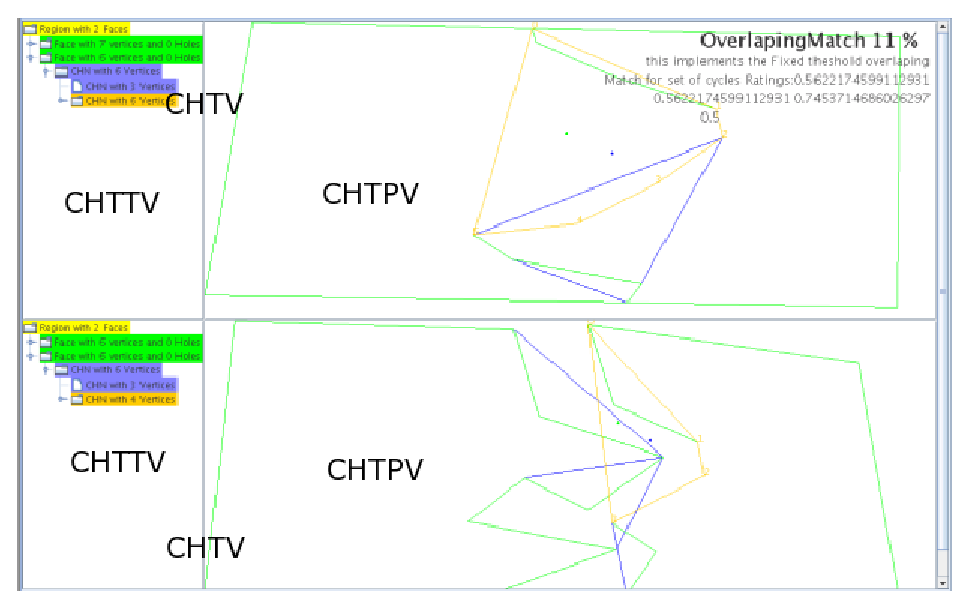
\includegraphics[scale=0.8]{MatchViewer.eps}
	\caption[Ein MatchViewer mit allen Unteklassen] {Hier sieht man die Komponenten MatchViewer, ConvexHullTreeViewer (CHTV), ConvexHullTreeTreeViewer (CHTTV) und ConvexHullPolygonViewer (CHTPV) zusammen.}
	\label{fig:MatchViewer}
\end{figure}

\item ConvexHullTreePolygonViewer

Diese Klasse dient dazu, einen RegionTree als Polygon darzustellen. Faces sind hier grün gefärbt, Holes rot und tierferliegende ConvexHullTreeNodes blau. Zu jedem ConvexHullTreeNode wird nicht nur der eigentliche Umfang des Polygons, sondern die Konvexe Hülle dargestellt.

Zusätzlich beinhaltet diese Klasse ein Attribut actual, das ein Feld von RegionTreeNodes ist. Diese Elemente werden organge dargestellt, und ermöglicht das Auswählen von Elementen, falls der ConvexHullTreePolygonViewer in einen höheren Kontext eingebunden wird.

\item ConvexHullTreeTreeViewer

Diese Klasse dient dazu, einen RegionTree als Baum darzustellen. Die Darstellung dieses Baumes orientiert sich an der Darstellung, win man sie von Verzeichnissbäumen in verschiedenen Betriebsystemen kennt.

Diese Klasse benutzt zwei Hilfsklassen:
\begin{itemize}
\item ConvexHullTreeTreeViewerNode

Diese Klasse repräsentiert einen Element des RegionTrees und kümmert sich zum einen um die textuelle Beschreibung dieses, und zum anderen darum, den Baum rekursiv aufzubauen.
\item ConvexHullTreeTreeViewerRenderer

Diese Hilfsklasse kümmert sich darum, die Darstellung der einzelnen Elemente farblich zu unterscheiden. Die Farben bei der Darstellung entsprechen denen im ConvexHullTreePolygonViewer, nur das zusätzlich noch die Farbe gelb, für das Vaterelement, die Region, benutzt wird.
\end{itemize}

Nachdem man ein Objekt dieser Klasse angelegt hat und ihm dabei den gewünschten RegionTree übergeben hat, läßt sich dieses wie jedes andere JPanel benutzen.

\item ConvexHullTreeViewer

Diese Klasse fasst die beiden Darstellungen als Baum und als Polygon zusammen. Auf der linken Seite dieser GUI-Komponente findet sich die Baum-Darstellung, und auf der rechten die Darstellung als Polygon. Die Verbindung zwischen den beiden wird hergestellt, so dass es möglich ist, in der Baumdarstellung ein, oder mehrere Nodes zu selektieren, die dann auch in der Polygondarstellung gesondert markiert werden.

\item MatchViewer

Dieses Control zeigt ein Match an, indem zwei ConvexHullTreeViewer, für die Source- und die Target-Region, übereinander dargestellt werden. Die Verbindung dieser beiden wird so umgeleitet, dass die Selektion eienes Elementes, in einem der beiden ConvexHullTreeTreeViewer die Selkektion in dem gematchten Element zu Folge hat. Konstruiert wird diese Komponente, indem man einfach ein Match übergibt. Auch diese Komponente ist von JPanel abgeleitet, und läßt sich entsprechend einsetzen.

\begin{figure}
	\centering
	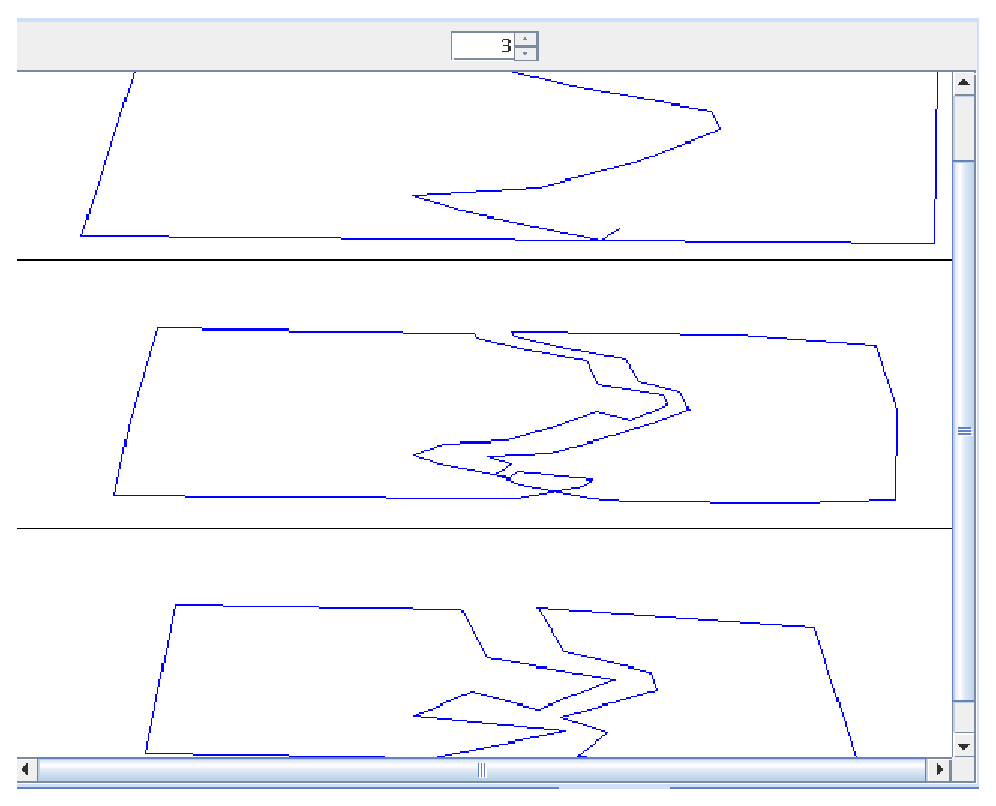
\includegraphics[scale=0.5]{Sectionviewer.eps}
	\caption{Ein SectionViewer, bestehend aus drei oneSectionViewern.}
	\label{fig:SectionViewer}
\end{figure}


\item SectionViewer

Diese Klasse stellt das Ergebniss des Matchings, die erzeugten dreidimensionalen Dreiecke dar, indem eine Menge von unterschiedlichen Schnittbildern dargestellt werden. Über ein Control läßt sich die gewünschte Anzahl der Schnittbilder einstellen und dann erscheinen diese im unteren Bereich der GUI-Komponente. Die einzelenen Schnittbilder werden von der Hilfsklasse  \textbf{oneSectionViewer} gezeichnet.

Konstruiert wird der Section-Viewer einfach, indem man diesem ein Objekt vom Typ mLineRep übergibt.


\item TriRepOutPutCanvas

Auch diese Klasse stellt ein mLineRep-Objekt dar. Allerdings erfolgt die Darstellung hier isometrisch. Die Source- und die Target-Region werden parallel zur Monitorebene dargestellt, wobei das target nach rechtsoben verschoben wird. Die Linien des Sources sind blau, die des Targets rot. Die Linien dazwischen, also die Linien der Dreiecke sind in grauer Farbe markiert.

Diese Komponente bekommt neben dem mLineRep-Objekt noch eine Ganzzahl, die den Grad der Verschiebung angibt. Diese läßt sich mittels der Methode \textbf{setTimeShift} auch nachträglich ändern. Auch wenn der Name der Klasse anderes vermuten läßt, ist diese Klasse kein Canvas sondern ein JPanel. Der Name ist noch ein Relikt von der T\o{}ssebroschen-Applikation.

\begin{figure}
	\centering
	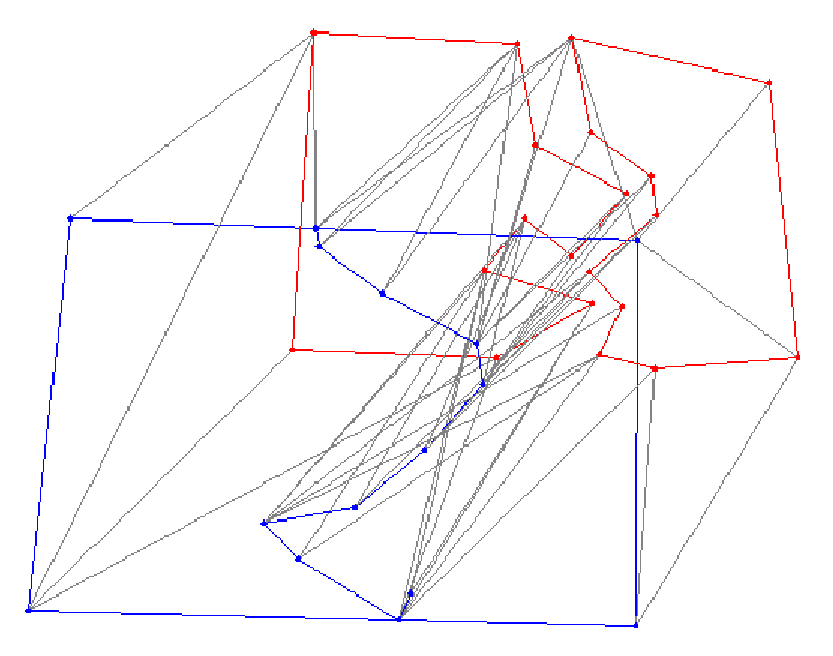
\includegraphics[scale=0.7]{TriRepOutPutCanvas.eps}
	\caption{Ein TriRepOutputCanvas.}
	\label{fig:TriRepOutputCanvas}
\end{figure}




\item tegnecanvas

Diese Klasse bildet die Zeichenfläche der Applikation. In dieser kann der Benutzer seine beiden Regionen malen. Nachdem der Benutzer dies getan hat, kann man mit den Funktionen getFirstSnapshot und getSecondSnapshot die Regionen auslesen. 

\item MCIContents

Diese Klasse vereinigt alle anderen Klassen zu der eigentlichen Applikation. Diese Klasse läßst sich entweder als Applet benutzen, oder in ein JFrame einbinden, der damit eine Standalone-Applikation bildet.
\end{itemize}
\section{Die Secondo-Algebra \anmerkung{3 Seiten}}\label{rialgebra}
\anmerkung{Hier beschreibe ich kurz, wie ich die Secondo-Algebra implementiert habe. Speziell die Einbettung in das Secondo soll hier betrachtet werden.}


%\chapter{Vom Matching zum MovingRegion}

%\printindex

%\nocite{KOP}
%\nocite{AAR}
%\nocite{Sch}
%\nocite{AHS}
%\nocite{BW}
%\nocite{Doe1}
%\nocite{Doe1a}
%\nocite{Doe2}
%\nocite{Schi}
%\nocite{Ber}
%\nocite{Lei}
%\nocite{Gru}
%\nocite{AFRW}
\nocite{FGNS}


\chapter[Experimente mit Regionen \anmerkung{ca. 5 Seiten}]{Experimente mit Regionen} \label{Kapitel4}
%\minitoc
%\newpage
\anmerkung{Hier werde ich "uber meine Erfahrungen im Umgang mit der neuen Algebra berichten. Zum Testen dienen verschiedene technisch interesannte Regionen. Besonders auf die G"ute der verschiedenen Matching-Verfahren in der Praxis werde ich hier eingehen.}
\chapter[Interpolation der Daten "uber Entwaldung]{Interpolation der Daten "uber die Entwaldung des Amazonasgebietes} \label{Kapitel5}
%\minitoc
%\newpage


\section{Die Datengrundlage}
Als Datengrundlage dienen Daten "uber die Entwaldung des Amazonasgebietes die in Form einer SEC"-ONDO-Daten"-bank zur Verf"ugung gestellt wurden. Die Daten aus den Jahren 2004 und 2005 entstanden im Rahmen des DETER-Programms.

\index{DETER}DETER (\textbf{De}tecção de Desmatamento em \textbf{Te}mpo \textbf{R}eal) ist ein Programm der \index{INPE}INPE (\textbf{I}nstituto \textbf{N}acional de \textbf{P}esquisas \textbf{E}spaciais), des brasilianischen Weltraumerforschungszentrums, zur Überwachung des Holzeinschlags am Amazonasgebiet. Der Fokus dieses Programms liegt auf der Erfassung kurzfristiger Veränderungen. \cite{DeF} führt näher aus:
\begin{quotation}
DETER for locations of new deforestation greater than
25 ha in near real-time every two weeks, are based on
a combination of medium and high resolution data using
a mixture model approach to identify changes in
fraction of bare soil and vegetation 
\end{quotation} 
DETER ist nicht unumstritten, \cite{Green} führt aus:
\begin{quotation}
Dieses System erfasst erfahrungsgemäß jedoch nur circa 40 Prozent der zerstörten Fläche.
\end{quotation} 

\newpage
Die DETER--Datenbank besteht aus mehreren Tabellen, die alle den gleichen Aufbau aufweisen. Jede Tabelle steht hierbei für einen Zeitpunkt, zu dem die Flächen aufgenommen wurden. Im Folgenden wird als Beispiel der Tabellenstruktur die Struktur der Tabelle vom 07.05.2004 dargestellt:
\begin{verbatim}
(OBJECT layer20040507 
        ()
        (
            (rel 
                (tuple 
                    (
                        (recordnumber int)
                        (shape region)
                        (layer string)
                        (layerno int))))))
\end{verbatim} 

\begin{figure}
	\centering
	\includegraphics[scale=0.55]{Aufbau_Deter.eps}
	\caption[Inkrementeller Aufbau der Deter--Daten]{Auf dieser Abbildung kann man gut den inkrementiellen Aufbau der Tabellen sehen. Die grünen Flächen entstammen der Aufnahme vom 07.05.2004 und die roten Flächen sind innerhalb von 14 Tagen dazugekommen.\\\textit{\begin{tabular}{ll}
Quelle: &Luftbild, Google Maps;\\
&DETER-Daten dargestellt mit SECONDO
\end{tabular}}}
	\label{fig:Inkrem}
\end{figure}
\newpage
\begin{itemize}
\item recordnumber

ist eine in jedem Layer eindeutige ID.
 
\item shape
 
ist das eigentliche Polygon als Region. Jede Region besteht hier nur aus einem einzigen Face.

\item layer

ist eine textuelle Beschreibung dieser Tabelle und entspricht dem Aufnahmedatum.

\item layerno 

ist eine fortlaufende Nummerierung der einzelnen Tabellen, beginnend mit der Früh"-esten und endend mit der Spätesten.

\end{itemize}
Die einzelnen Layer sind inkrementiell aufgebaut, in dem zweiten Layer sind also nur die Flächen aufgeführt, die seit der letzten Erfassung dazugekommen sind. Dass bei diesem Aufbau Entwaldungsflächen nicht schrumpfen können, ist dem Problem leider angemessen. Abbildung~\vref{fig:Inkrem} veranschaulicht diesen Aufbau.


Die Anzahl der einzelnen Flächen in der Datenbank beträgt insgesamt 30.484, verteilt auf 19 Layer. Auf jeden Layer entfallen also durchschnittlich 1.600 Flächen.
 
Betrachtet wurde der Zeitraum zwischen 07.05.2004 und 30.09.2005.

\section{Die Aufarbeitung der Daten}

Das erste Problem bei der Verarbeitung der Daten ist die zu kleinteilige Erfassung der Polygone der einzelnen Layer. Es gibt in jedem Layer mehrere Polygone, die direkt nebeneinander liegen bzw. sich sogar überlappen. Für eine erfolgreiche Weiterverarbeitung ist eine Zusammenfassung dieser Polygone erforderlich.

Das nächste Problem ist, dass die einzelnen Layer inkrementiell aufgebaut sind, also die Beobachtung zu einem bestimmten Datum aus allen älteren Layern mit dem aktuellen zusammengesetzt werden muss.

In einem ersten Schritt müssen also neue Layer erzeugt werden, so dass gilt:

\begin{enumerate}
\item Ein neues Layer muss die Daten des nächstälteren Layer und Daten des Zieldatums enthalten.
\item In dem neuen Layer müssen alle benachbarten Polygone zu einem Einzigen vereinigt werden.
\end{enumerate}

Am Beispiel des 21.05.2004 werden im Folgenden werden die konkreten Schritte angegeben, um einen neuen Layer zu erzeugen.
\begin{enumerate}
\item  Zuerst müssen die Layer \textbf{layer20040507b} und \textbf{layer20040521} vereinigt werden. Bei dem ersten Layer überhaupt kann dieser Schritt natürlich entfallen. Dies leistet die Anweisung: 

\begin{verbatim}
let tmp = layer20040507b feed layer20040521 feed mergeunion consume
\end{verbatim}
\item Im nächsten Schritt werden alle zusammengehörigen Polygone zusammengefasst.

\begin{verbatim}
let tmp2 = connectedcomponents (
tmp feed {s} tmp feed {t} spatialjoin [shape_s,shape_t] 
constgraph [recordnumber_s,recordnumber_t,fun (i:int) 1.0] ) 
extend [shape: vertices (.Graph) extend [Key:key (.Vertex) ] 
tmp feed 
sortmergejoin [Key,recordnumber] 
aggregateB [shape; fun (r1:region,r2:region) 
union_new (r1,r2); [const region value()] ] ] 
project [shape] consume
\end{verbatim}
Der \textit{spatialjoin} von \textbf{tmp} mit sich selbst liefert alle Paare von zusammengehörigen Polygonen, die dann als Kanten in einem Graphen eingetragen werden, der mittels \textit{constgraph} erzeugt wird. Die Zusammenhangskomponenten dieses Graphen sind nun die zusammengehörigen Polygone. Jede Zusammenhangskomponente wird mit \textit{vertices} in seine Ecken zerlegt, die mit \textit{key} in einen Strom von ID's zerlegt werden. Dieser Strom wird mittels \textit{sortmergejoin} mit den Polygonen aus \textbf{tmp} verbunden. Jeder dieser Teilströme wird dann unter Zuhilfenahme von \textit{aggregateB} und \textit{union\_new} zu einem einzelnen Polygon verbunden. Der nicht mehr benötigte Graph wird am Schluss mit \textit{project} verworfen.

\item Um die \textbf{recordnumber} Felder disjunkt zu halten, läßt man die neuen ID's mit $layerno\times 10.000$ beginnen.

\begin{verbatim}
query seqinit(20001)
\end{verbatim}
\item Um die ursprüngliche Struktur der Tabelle wiederherzustellen, ergänzt man die Attribute \textbf{recordnumber}, \textbf{layer} und \textbf{layerno} und stellt die Reihenfolge der Attribute wieder her.

\begin{verbatim}
let layer20040521b = tmp2 feed extend [recordnumber: seqnext(),
layer: "layer20040521", layerno: 2] 
project [recordnumber, shape, layer, layerno] consume
\end{verbatim}
\end{enumerate}

\section{Die Konstruktion der Region-Units}
Um die Region--Units konstruieren zu können wird nun eine Tabelle aufgebaut, die zu jeder \textit{Region} des aktuellsten Layers die Vereinigung aller \textit{Regionen} beinhaltet, die mit zu dieser in einem räumlichen Bezug stehen. 

\begin{verbatim}
let layer20040608c = layer20040608b feed {n} layer20040521b feed {a} 
spatialjoin [shape_n,shape_a] 
sortby[recordnumber_n,recordnumber_a] rdup 
groupby[recordnumber_n; shape_n : group feed extract[shape_n], 
shape_a : group feed 
aggregateB [shape_a; fun(r1 : region, r2 : region) 
union_new (r1, r2); [const region value()] ] ] consume
\end{verbatim}

Hierzu wird zunächst ein \textit{spatialjoin} über die beiden Tabellen ausgeführt. Das Ergebnis wird sortiert und eventuell vorkommende Duplikate werden gelöscht. Dann erfolgt eine Gruppierung nach der \textbf{recodnumber} des neueren Layers. Das neue Element \textbf{shape\_n} wird erzeugt, indem das erste Element \textbf{shape\_n} der Gruppe genommen wird. Da nach der entsprechenden \textbf{recordnumber} gruppiert wurde sind all diese Elemente gleich. Das neue Element \textbf{shape\_a} wird erzeugt, indem alle älteren Regionen der Gruppe vereinigt werden.

Mit Hilfe des neugeschriebenen \textit{interpolate} Operators lassen sich nun Region--Units erzeugen. Hierzu wird die Tabelle um die Spalte \textbf{RegionUnit} erweitert. In dieser wird, mit Hilfe von \textit{interpolate}, aus den beiden Regionen \textbf{shape\_a} und \textbf{shape\_n}, die neue Region--Unit erzeugt. Das Zeitintervall muss leider händisch angegeben werden, da die Konstruktoren von \textit{Instant} das Datum nicht aus der Zeichenkette in \textbf{layer} gewinnen können.
\begin{verbatim}
let layer20040608d feed 
extend[RegionUnion : interpolate(
.shape_a, .shape_n,
theRange(theInstant(2004, 5, 21), theInstant(2004, 6, 8), TRUE, FALSE))] 
consume
\end{verbatim}

\begin{figure}
\centering
\subfigure{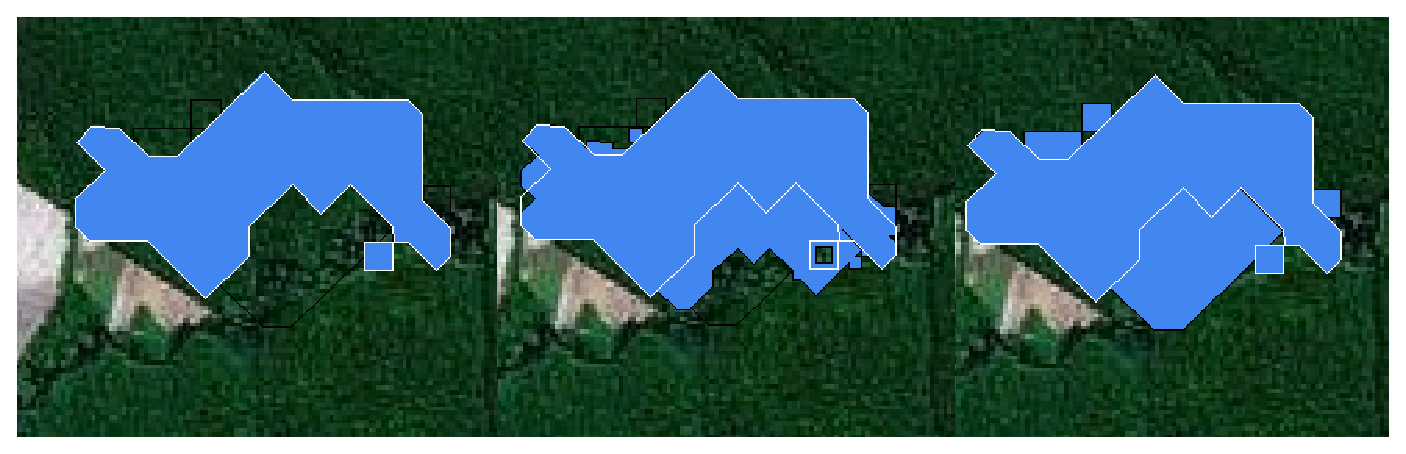
\includegraphics[width=0.9 \textwidth]{DeterUnit.eps}}
\subfigure{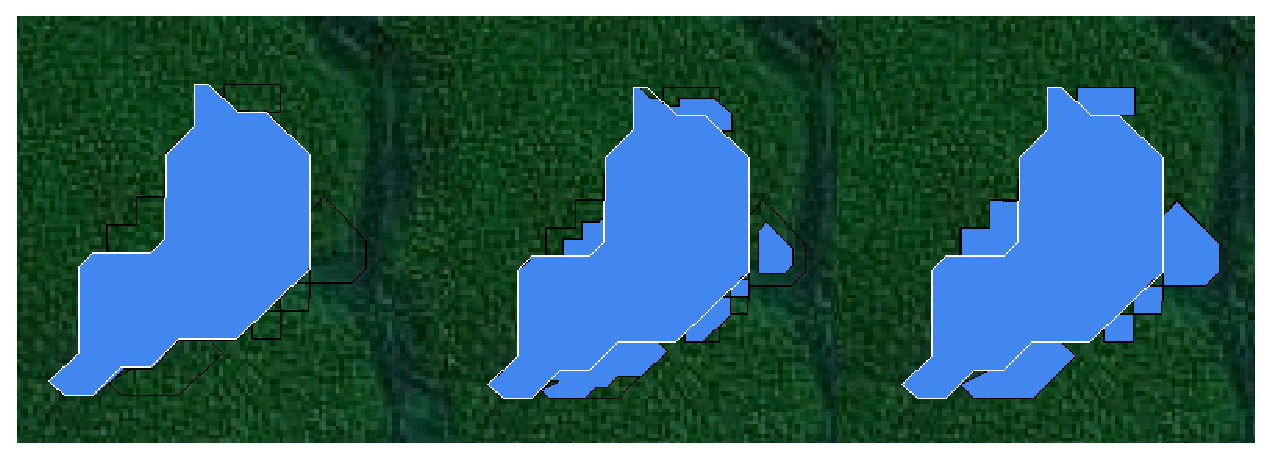
\includegraphics[width=0.9 \textwidth]{DeterUnit2.eps}}		\subfigure{\includegraphics[width=0.9 \textwidth]{DeterUnit3.eps}}		
	\caption[Region--Unit aus Deter--Daten]{Je drei Momentaufnahmen dreier Region--Units, die aus den Deter--Daten gewonnen wurden.\\\textit{\begin{tabular}{ll}
Quelle: &Luftbild, Google Maps;\\
&DETER-Daten dargestellt mit SECONDO
\end{tabular}}}
	\label{fig:RegionUnitDeter}
\end{figure}


%\section{Die Konstruktion der Moving-Regions}


\chapter[Ausblick ]{Ausblick} \label{Kapitel6}

\section*{Rückblick}

In der Einleitung, Kapitel~\vref{Kapitel1}, wurden zwei Beispiele für Moving--Regions gegeben und die Frage gestellt, ob es gelingen würde aus diesen Unwetter--Daten beziehungsweise den DETER--Daten kontinuierliche Bewegungen zu erzeugen. 

Zum ersten Beispiel kann nun gesagt werden, dass die Erzeugung prinzipiell gelingen würde (Falls das Beispiel nicht ein komplett fiktives wäre.). Jedoch würden bei Wetterdaten, die stark rotierende Daten sind die Probleme aus ~\vref{ProblemeRotation} zum Tragen kommen. In Abbildung~\vref{fig:Wetterdaten} wurde versucht, den Charakter von sich bewegenden Luftdruckgebieten zu treffen. Man kann gut sehen, dass die Interpolation zwar gelingt, das Ergebnis nach der Hälfte der Zeit aber viel zu groß ist und den beiden \textit{Faces} nicht stark ähnelt.

\begin{figure}
	\centering
	\includegraphics[scale=0.8]{Wetterdaten.eps}
	\caption[Bewegende Wetterdaten]{Fiktives Beispiel für bewegende Wetterdaten\\\textit{Quelle: Eigene Darstellung}}
	\label{fig:Wetterdaten}
\end{figure}
Beim zweiten Beispiel, den DETER--Daten, ist Überführung der Daten in eine kontinuierliche Form möglich, wie in Kapitel~\vref{Kapitel5} geschehen.


Auf dem Weg zur Lösung dieser Probleme wurden zwei verschiedene Applikationen erzeugt, das Java--Applet und die SECONDO--Algebra. 
Die Java-Applikation entstand nur aufgrund der Tatsache, dass es bereits eine solche Applikation gab, die von Erlend T\o{}ssebro entwickelt worden war. Diese Applikation wurde von dem Autor dieser Arbeit erweitert, so dass diese nun die Problemstellung der Arbeit löst. Obwohl diese Applikation nicht gefordert war, ist dieses Programm nicht überflüssig, es zeigt didaktisch gut aufbereitet wie das Matching passiert.

Die SECONDO--Algebra integriert die Möglichkeit zur Berechnung von kontinuierlichen Bewegungen in das SECONDO--System. Innerhalb dieses System ist es nun also möglich Regionen zu interpolieren. Aus technischen Gründen wurde dieser eine Operator als eigene Algebra implementiert, eine spätere Integration dieses Operators in die Moving--Region--Algebra ist aber möglich.




\section*{Probleme}
Sowohl bei der Bestimmung von Matchings mittels des Overlapping--Matches, als auch bei der Berechnung der entsprechenden Overlap--Bewertung, wird die Intersection--Funk"-tion der MakeOp-Klasse verwendet. Diese findet sich in der Plane--Sweep--Algebra. Leider führte die Verwendung dieser Funktion immer wieder zu Abstürzen, wie sie auch bei der Verwendung des \textit{union\_new} Operators derselben Algebra auftauchen. Deshalb wurde es leider nötig, auf diese Verfahren zu verzichten. Wenn die Probleme mit der externen Algebra behoben sind, kann man diese Verfahren einfach wieder reaktivieren, indem man in der Datei ,,RegionInterpolator.h'' die folgende Zeile wieder einkommentiert.
\begin{verbatim}
#define USE_OVERLAP
\end{verbatim}  

\section*{Erfahrungen}

In \vref{Zerlegung} wurde ein Algorithmus vorgestellt, der ein Polygon in konvexe Polygone zerlegen kann. Der Algorithmus wurde in der Hoffnung entwickelt, eine wesentlich weniger kleinteilige Zerlegung der Polygone zu erreichen, als das eine Triangulierung liefern würde. In der praktischen Erfahrung zeigt sich aber, dass die Zerteilung bei realen, komplizierten \textit{Faces} mit \textit{Holes} doch sehr kleinteilig wird. Abbildung~\vref{fig:ZerlegungFace2} zeigt ein solches Beispiel.

Die Verwendung dieses Algorithmus kann deshalb nicht uneingeschränkt empfohlen werden. Falls nicht klar ist, wie kompliziert die zu zerlegenden Polygone aufgebaut sind, so empfiehlt sich eher die Verwendung eines performanten Triangulierungs--Algorithmus. Ein solcher Algorithmus wird etwa unter \cite{Sei} vorgestellt.


\begin{figure}
	\centering
	\includegraphics[scale=0.9]{Convexer.svg.eps}
	\caption[Zerlegung eines Polygons, nur wenig besser als eine Triangulierung]{Ein Beispiel, in dem die Zerlegung eines Polygons Zerlegung liefert, die kaum besser als eine Triangulierung ist. Ein einziges Viereck ist das einzige vorkommende Polygon, das kein Dreieck ist.\\\textit{Quelle: Eigene Darstellung}}
	\label{fig:ZerlegungFace2}
\end{figure}

\section*{Raum für weitere Überlegungen}

Obwohl die implementierten Matchings bereits gute Ergebnisse liefern, kann man die entsprechende SECONDO--Algebra als Framework begreifen, um andere vielversprechende Matchings zu implementieren. Bei der Imlementierung der Algebra wie auch der Java--Applikation wurde auf eine guter Erweiterbarkeit geachtet, so dass eine Implementierung komplexerer Matching-Verfahren mit geringem Aufwand möglich ist. Es erscheint durchaus empfehlenswert, die eigenen Ideen zuerst in der Java--Applikation zu entwickeln, da diese viele Möglichkeiten des optischen Debuggen bietet. Im Anhang~\vref{eigeneMatch} wird beschrieben, wie man eigene Verfahren zum Matchen und Bewerten  implementieren, und wie man diese Verfahren in die Algebra einbauen kann.

Im Laufe der Arbeit wurden bereits einige Verfahren aufgezeigt, die eventuell gute Matches liefern können:
\begin{itemize}
\item Algorithmen zum Finden von pseudooptimalen Lösungen

In \vref{AARR} und \vref{AFRWW} wurden die Algorithmen aus den Veröffentlichungen \cite{AAR} und \cite{AFRW} vorgestellt. Diese Algorithmen könnten sehr gute Ergebnisse mit vertretbaren Aufwänden liefern. Da diese Paper aber eher aus dem Bereich der Mustererkennungen kommen, kümmern sich diese nur um 1:1 Matches.  Wie man mit diesen Algorithmen auf Vereinigungen und Zersplitterungen reagieren kann, muss noch überlegt werden.

\item Bewertung mittels $\min_{T\in\mathcal{T}}\delta(A,T(B))$

Das Verfahren, welches im letzten Abschnitt beschrieben wurde, liefert auch die Möglichkeit, gegebene 1:1 Matches zu bewerten. Eine diesbezügliche Implementierung wird voraussichtlich gute Ergebnisse bieten. 

\item statistisches Referenzpunktverfahren

In \vref{StatistikAlgo} wurde ein Verfahren aufgezeigt, das mittels statistischer Analyse aus einer Menge von Referenzpunkten zusammengehörige Cluster finden kann. Möglicherweise könnte dieses Verfahren gute Ergebnisse liefern, die Laufzeit wird aber nicht besonders gut sein.

\item Verfahren mit neuronalen Netzen oder mit Support--Vector--Maschinen

Unter \vref{neuroNetz} wurde auch ein Verfahren andiskutiert, das eine Gruppenbildung auf einer Menge von Referenzpunkten mittels neuronaler Netze oder Support--Vector--Maschinen durchführt. Weitere Überlegungen in dieser Richtung, zu Laufzeiten oder Qualitäten, wurden nicht angestellt. 
 
\item Maximize Overlap (set of cycles)

In \cite{TG} wird ein Matching--Verfahren entwickelt, das zwei Flächen matched, wenn Ihre Überlappung maximal ist. Dieses Verfahren ist unter Kapitel~\vref{MaxOver} näher beschrieben. Auch dieses Verfahren wurde nicht implementiert, könnte aber zu interessanten Ergebnissen führen.
\end{itemize}





\begin{appendix} \label{anhang}
\part*{Anhänge}
\mtcaddpart[Anh"ange]
\adjustptc[-2]
\parttoc

 
\chapter{Anleitung zur Benutzung des Java-Interpolators}\label{Handbuch}
\minitoc
\newpage
\section{Einleitung}
Im Rahmen dieser Diplomarbeit entstand neben einer neuen Algebra f"ur SECONDO, auch eine Java-Anwendung, die dieselbe Arbeitsweise wie die Algebra aufweist. Die Benutzung dieses Tools wird im Folgenden erl"autert.

Das Tool dient in erster Line dem besseren Verst"andnis, wie die Algebra funktioniert. Ein Import oder Export mit SECONDO ist nicht m"oglich.

\section{Starten des Tools}
Das Tool ist in Java geschrieben und liegt als Jar-Datei vor. Um das Programm ausf"uhren zu k"onnen, muss deshalb eine Java Laufzeitumgebung ab Version~1.4 vorhanden sein. Ist dies der Fall, so l"asst sich das Programm mittels \begin{verbatim}
java -jar MCInterpolator.jar
\end{verbatim}  starten.

Es erscheint der Startbildschirm, der in Abbildung~\vref{fig:start}dargestellt wird.

Dieser l"asst sich in vier Bereiche unterteilen:
\begin{itemize}
\item Eine Toolbar, die den VRML-Export Button und den Zeit-Einsteller beinhaltet. 
\item Die Zeichen-Toolbar wozu sich nähere Informationen im Kapitel ,,Zeichnen einer Region`` finden.
\item Der Zeichenbereich wo man neue Regionen zeichnen kann und importierte Regions betrachtet.
\item Die Umschaltfl"achen  mit denen zwischen den verschiedenen Werkzeugen gewechselt werden kann. Nach dem Starten findet sich hier neben der Zeichenf"ache nur Konfigurationsschaltfl"ache, die im Kapitel ,,Konfigurieren des Matchings`` n"aher beschrieben werden. Schlie"st man die Zeichnung von zwei Regions ab, tauchen weitere Schaltfl"achen auf, die im Kapitel ,,Die verschiedenen Ergebnisansichten`` erl"autert werden.
\end{itemize} 

\begin{figure}
   \centering
   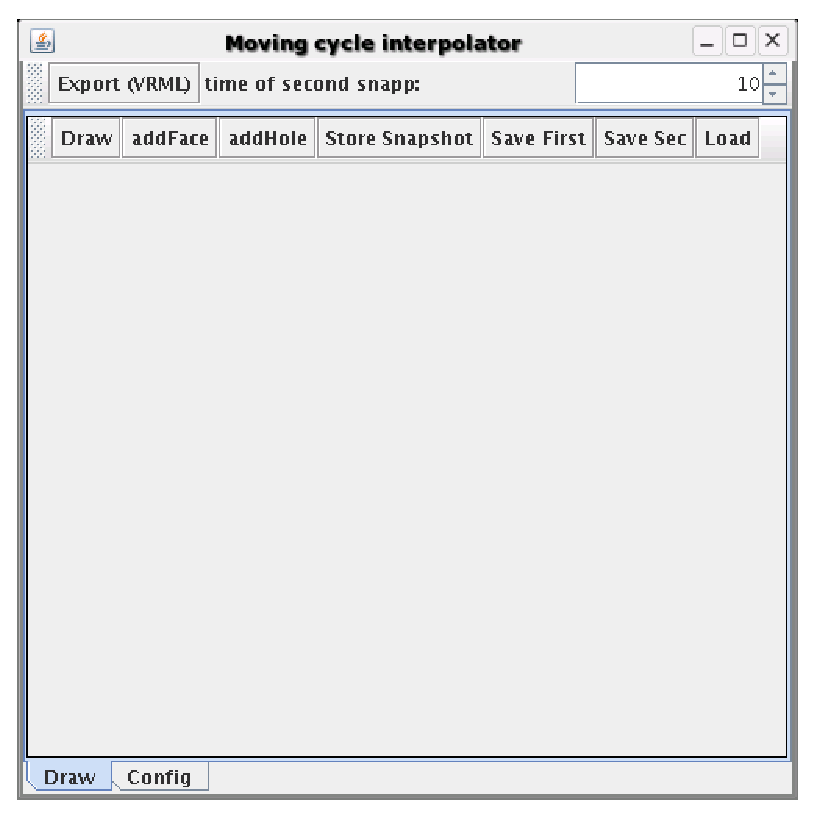
\includegraphics[scale=.8]{/home/java/Documents/Tex/Tex/start.eps}
   \caption{Der Startbildschirm}
   \label{fig:start}
\end{figure}

\section{Zeichnen einer Region}
Direkt nach dem Starten der Anwendung kann man anfangen, das erste Face zu zeichnen.  Das Zeichnen geht immer so vor sich, dass man die Punkte des Polygons nacheinander mit der Maus anklickt. Der neue Punkt und die dazugeh"orige Linie werden direkt dargestellt. 

Das Polygon muss nicht geschlossen werden, aber es ist zu beachten, dass alle Polygone einfache Polygone sein m"ussen. Eine entsprechende "Uberpr"ufung findet nicht statt.

Zum Zeichnen einer Region stehen folgende Werkzeuge bereit:
\begin{itemize}
\item Draw

Dieser Button l"oscht alle bereits eingegebenen Zeichnungen und hinterl"asst ein leeres Zeichenblatt. Auch die eventuell bereits vorhandenen Schaltfl"achen f"ur die Ergebnisansichten werden ausgeblendet.

\item addHole

Hiermit kann man dem letzten Face ein Hole hinzuf"ugen. Holes unterscheiden sich von Faces darin, dass sie nicht blau sondern rot sind. Ein Hole muss komplett innerhalb seines Faces liegen. Dies sicherzustellen ist die Aufgabe des Benutzers, eine "Uberpr"ufung findet nicht statt.

\item StoreSnapshot

Soll die Zeichnung einer Region beendet werden, so muss auf diesen Button geklickt werden. Falls es der erste Schnappschuss ist, der beendet wird, so f"arbt sich dieser blasser, und man  kann den n"achsten zeichnen. Wird aber der zweite beendet, so wird das passende Match berechnet und in den zus"atzlichen Schaltfl"achen dargestellt, die sich in ,,Die verschiedenen Ergebnisansichten`` finden.
\end{itemize} 

\section{Importieren / Exportieren}
Zum Importieren und Exportieren von Schnappsch"ussen, die mit diesem Programm erzeugt wurden, stehen drei Schaltfl"achen zur Verf"ugung:

,,Save First``, ,,Save Sec`` und ,,Load``. Wird auf einen der beiden Save-Buttons gedrückt, so "offnet sich ein Dateiauswahl-Dialog, in dem ein Dateiname f"ur die Schnappschuss-Datei angeben werde kann.

Mit Hilfe des Load-Buttons k"onnen dann diese Schnappsch"usse einzeln wieder geladen werden. Falls bereits zwei Schnappsch"usse in dem Programm sind, so muss man ,,Draw`` dr"ucken, bevor neue Dateien einlesen.
\section{Konfigurieren des Matchings}
Hinter der Schaltfl"ache ,,Config`` verbirgt sich ein Dialogfenster (siehe Abbildung \vref{fig:Config}), in dem einige Einstellungen vorgenommen werden k"onnen:

\begin{itemize}
\item VRML Filename und VRML Application

Erl"auterungen zu diesen Feldern befinden sich in dem Unterkapitel ,,Die verschiedenen Ergebnisansichten / VRML-Export``

\item Auswahlfeld f"ur die Art des Matchings

Hier kann man ausw"ahlen, welches Matching man gerne ausf"uhren m"ochte. Die zur Zeit verf"ugbaren Matching-Methoden werden in der Arbeit ausf"uhrlich erl"autert.

\item Schieber f"ur die Parameter der Einzelmatches

Hier kann man einigen Einzel-Matches, zur Zeit dem OverlappingMatch und den Referenzpunktverfahren, einen Parameter "ubergeben. Hierbei ist zu beachten, dass dieser Parameter je nach Art des Matches unterschiedliche Auswirkungen hat.

\item Schieber f"ur die Parameter des Optimalmatches

Das \textit{OptimalMatch} setzt sich aus den EinzelMatches zusammen, indem es verschiedene Einzelmatches mit verschiedenen Parametern ausf"uhrt und dann bewertet. In diese Bewertung flie"sen mehrere Kriterien gewichtet ein. Mit Hilfe dieser Schieber lassen sich die Gewichtungen der Einzel-Kriterien ver"andern.

\item Die Einzel-Bewertungen des Matches

In diesen Feldern sind die Bewertungen des aktuellen Matches,nach den einzelnen Kriterien, aufgeschl"usselt.
\end{itemize} 
\begin{figure}
   \centering
   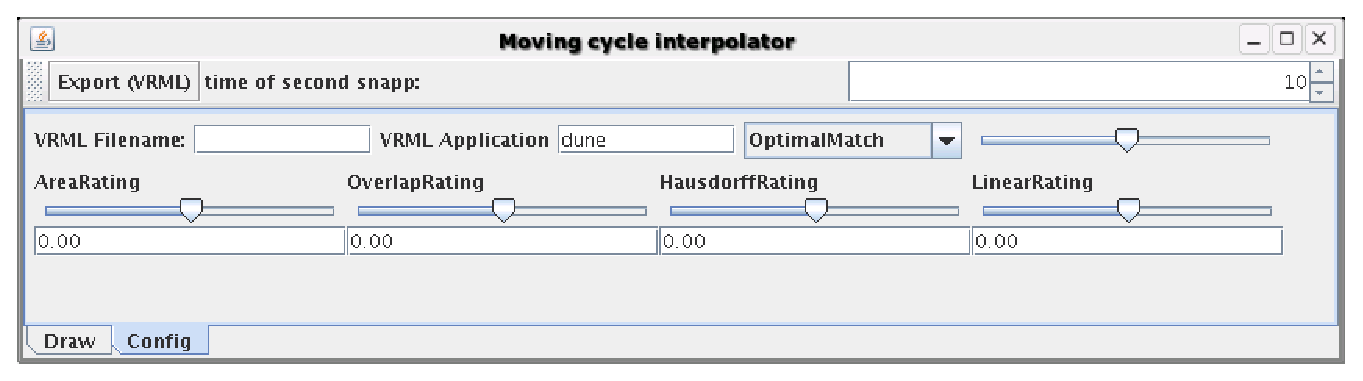
\includegraphics[scale=.65]{/home/java/Documents/Tex/Tex/Config.eps}
   \caption{Der Config-Dialog}
   \label{fig:Config}
\end{figure}
\section{Die verschiedenen Ergebnisansichten}
Sobald der zweite Schnappschuss geschlossen wird, erscheinen einige neue Schaltfl"achen, in denen  das Resultat des Matchings zu sehen ist.

Bei den Erl"auterungen dieser Schaltfl"achen werden die Schnappsch"usse, die in Abbildung~\vref{fig:Splits} dargestellt sind, benutzt.
\begin{figure}
   \centering
   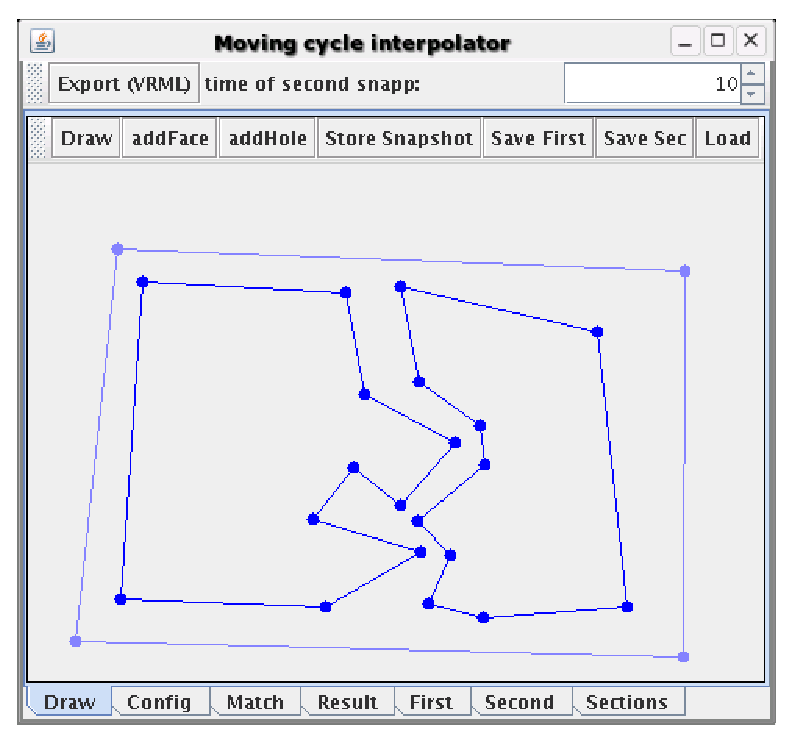
\includegraphics[scale=.8]{/home/java/Documents/Tex/Tex/Splits.eps}
   \caption{Das Beispiel}
   \label{fig:Splits}
\end{figure}
\subsection{Match}
In diesem Bildschirm (siehe Abbildung~\vref{fig:Match}) finden sich die beiden Schnappsch"usse in derselben Darstellung wie in ,,First`` und ,,Second``. In dem entsprechenden Kapitel wird diese Darstellung n"aher erl"autert. 

W"ahlt man ein Element in einer der beiden Darstellungen aus, so wird das gematchte Element der anderen Darstellung selektiert. 

In der rechten oberen Ecke des Fensters befindet sich der Name des \textit{Matches}, eine Erl"auterung zu diesem und die Bewertung in den Kategorien. Im Falle eines \textit{OptimalMatches} findet sich hier eine Liste mit allen Einzelmatches, die zu diesem Ergebnis kommen.
\begin{figure}
   \centering
   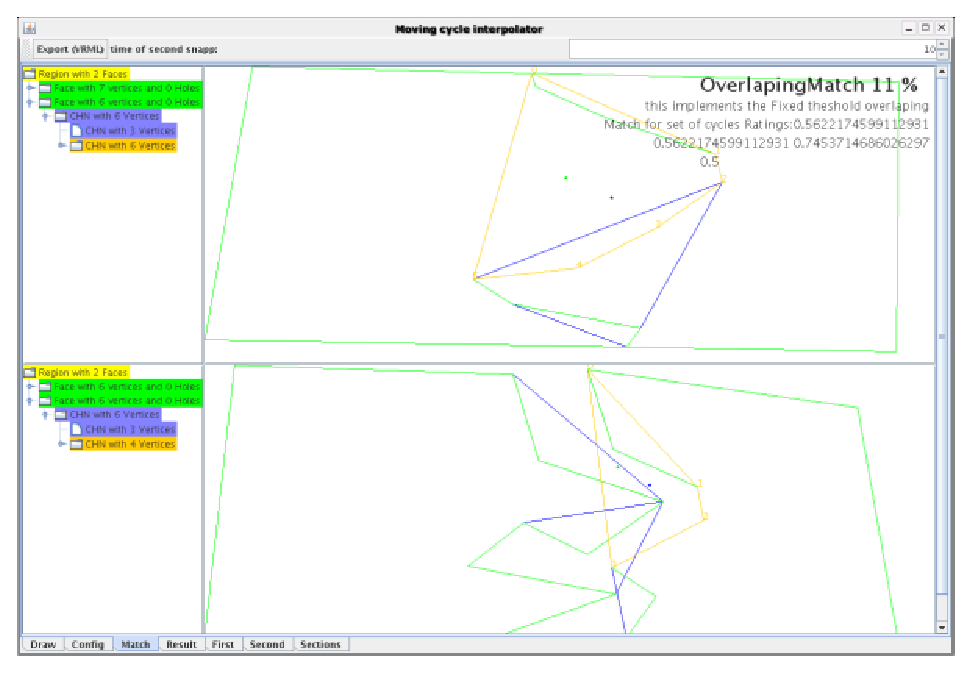
\includegraphics[scale=.8]{/home/java/Documents/Tex/Tex/Match.eps}
   \caption{Die Match-Darstellung}
   \label{fig:Match}
\end{figure}

\subsection{Result}
In diesem Bildschirm (siehe Abbildung \vref{fig:Result}) findet man eine isometrische Darstellung des Matches. Hier kann man  beide Schnappsch"usse wiederfinden. Der erste ist blau gezeichnet, der zweite rot. Die Linien, die die beiden verbinden, sind grau. 

Mit Hilfe des Zeit-Einstellers in der obersten Toolbar kann der zweite Schnappschuss weiter nach hinten rechts verschoben bzw. zur"uckgeholt werden. 

\begin{figure}
   \centering
   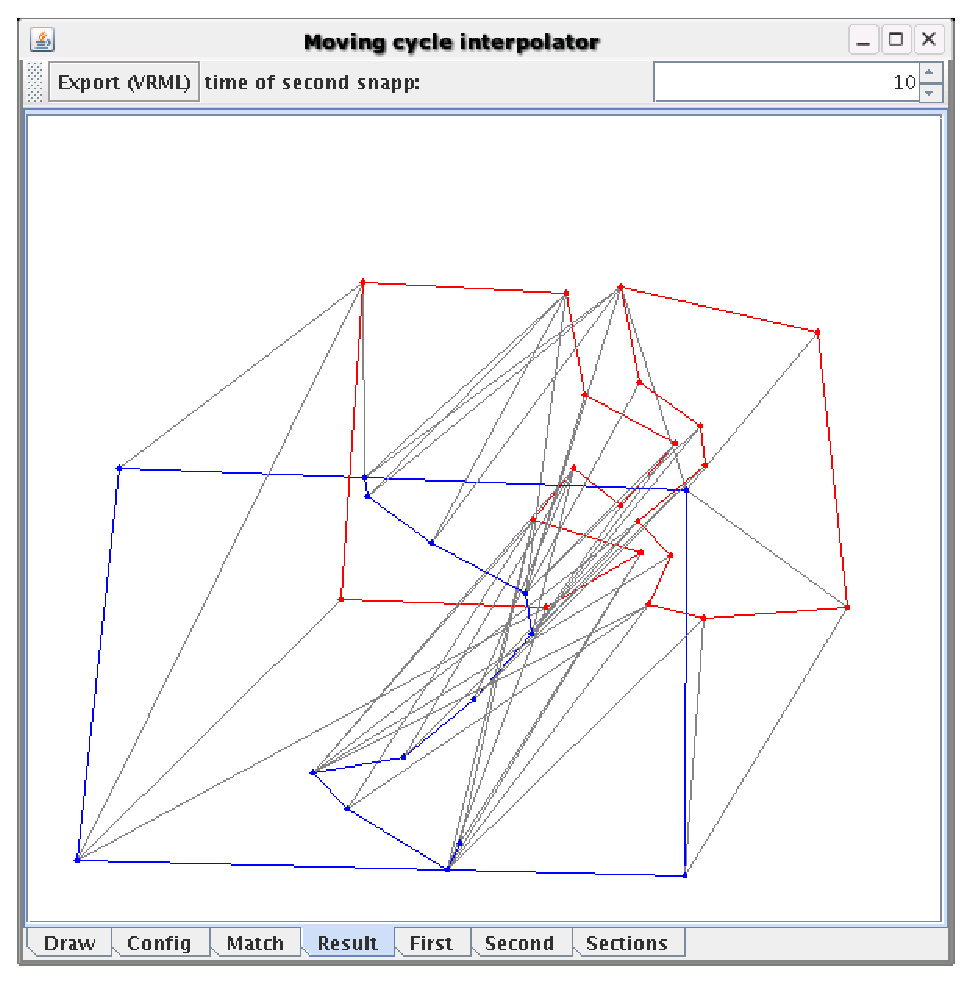
\includegraphics[scale=.6]{/home/java/Documents/Tex/Tex/Result.eps}
   \caption{Die Result-Darstellung}
   \label{fig:Result}
\end{figure}
\subsection{First und Second}
In dieser Ansicht (in Abbildung \vref{fig:Second} findet sich ,,Second`` als Beispiel) findet man zwei Darstellungen des \textit{ConvexHullTrees} eines Schnappschusses. Links befindet sich eine Baum\-ansicht des \textit{ConvexHullTrees}.

Diese Darstellung erm"oglicht es, in dem Baum zu navigieren und Elemente zu selektieren. Mehrfachselektionen kann man vornehmen, indem man beim Klicken die Strg oder die Umschaltaste h"alt. Die einzelnen Elemente des Baumes sind farblich zu unterscheiden.

Die Farben bedeuten:
\begin{itemize}
\item Gelb Region
\item Gr"un Face
\item Blau ConvexHullTreeNode
\item Rot Hole
\item Orange Selektion
\end{itemize} 

Rechts befindet sich eine Darstellung des Baumes als Menge von Polygonen. Die Farbgebung entspricht der oben genannten, allerdings ist die Region nicht extra dargestellt. Jedes \textit{Face} ist durch das Polygon seines \textit{Cycles} dargestellt, jedes Element eines \textit{ConvexHullTrees}, einschlie"slich der \textit{Holes}, ist durch seine konvexe H"ulle dargestellt. Selektiert man ein Element in der Baumansicht, so f"arbt sich dieses orange, die Ecken der konvexen H"ulle werden durchnummeriert und Schwerpunkt (blau) und Steiner-Punkt (gr"un) werden dargestellt.

\begin{figure}
   \centering
   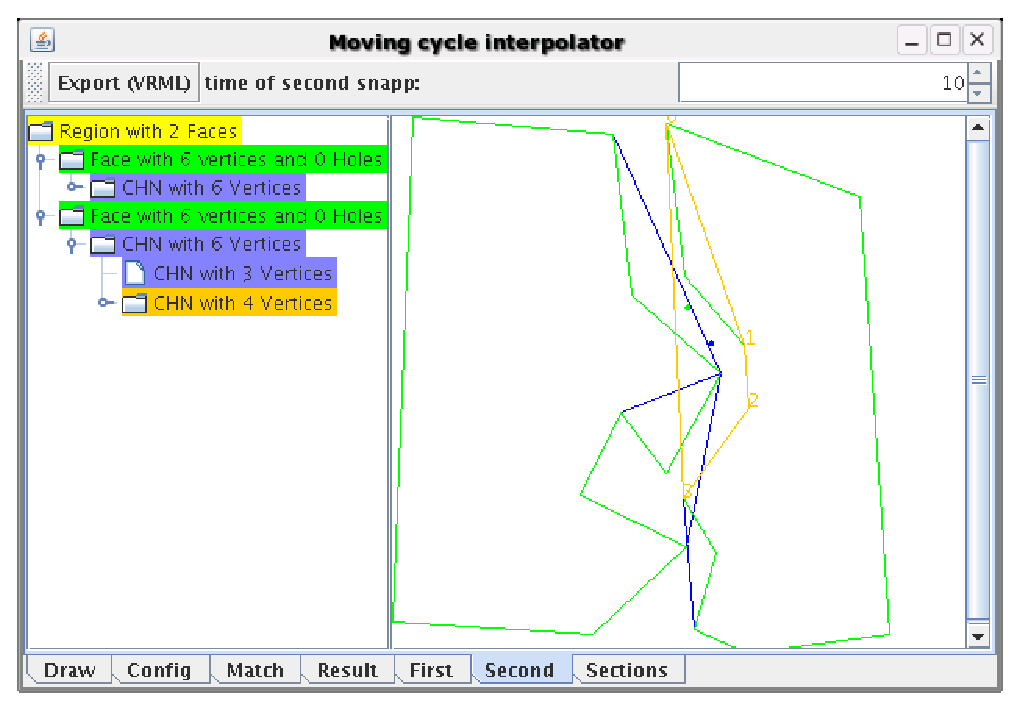
\includegraphics[scale=.8]{/home/java/Documents/Tex/Tex/Second.eps}
   \caption{Die ConvexHullTree-Darstellung des zweiten Schnappschusses}
   \label{fig:Second}
\end{figure}
\subsection{Sections}
In dieser Darstellung (Abbildung \vref{fig:Sections}) befinden  sich interpolierte Schnappsch"usse, die aus dem Match erstellt wurden. In dem Feld mittig "uber der Darstellung kann gew"ahlt werden, wieviele Schnappsch"usse betrachtet werden sollen.

Diese tauchen dann in dem Zeichenbereich dieser Seite auf. Der erste und der letzte entsprechen dem ersten und dem zweiten Schnappschuss.
\begin{figure}
   \centering
   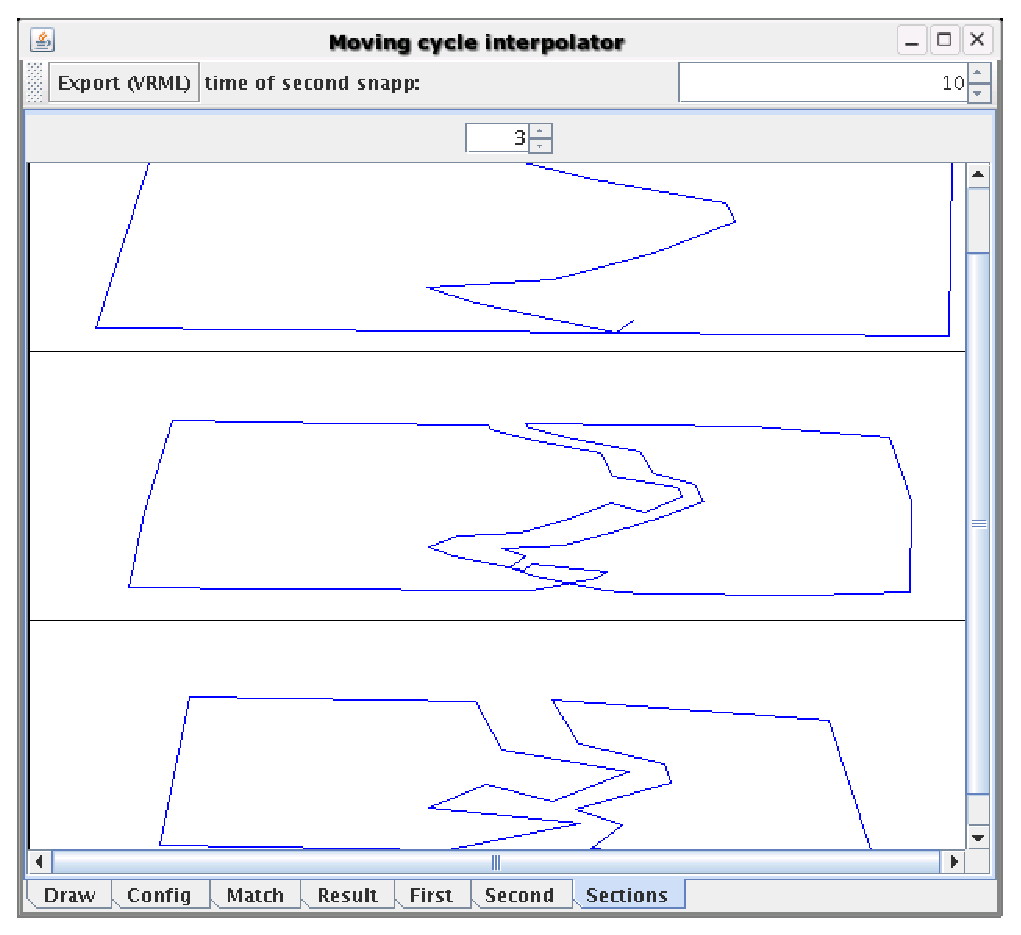
\includegraphics[scale=.8]{/home/java/Documents/Tex/Tex/Sections.eps}
   \caption{Drei Sections unseres Beispieles}
   \label{fig:Sections}
\end{figure}
\subsection{VRML-Export}
Das Tool bietet die M"oglichkeit, ein Match in eine VRML-Datei zu exportieren und so eine ansprechende 3D-Darstellung zu erhalten. Zu dem VRML-Export geh"oren vier GUI-Elemente:
\begin{itemize}
\item VRML Filename im Config-Dialog

 In diesem Feld kann man den gew"unschten Dateinamen angeben, den die neue VRML-Datei bekommen soll. Die Erweiterung .vrml wird automatisch erg"anzt
\item VRML Application im Config-Dialog

Tr"agt man in diesem Feld einen Konsolenbefehl ein, mit dem man einen VRML-Viewer startet, so startet das Tool diesen Viewer direkt nach dem Export mit der neuen Datei.

\item Der ,,Zeit-Einsteller`` in der obersten Toolbar

Mit diesem Control kann die ,,H"ohe`` der 3D-Darstellung bestimmt werden. Kleine Werte f"uhren zu flachen Polyedern, gro"se zu hohen.
\item Der ,,Export (VRML)``--Button in der obersten Toolbar

Durch den Klick auf diesen Button wird der Export ausgel"ost. Die VRML--Datei der gew"unschten H"ohe und mit dem gew"ahlten Namen wird erzeugt und direkt in dem Viewer der Wahl ge"offnet.
\begin{figure}
   \centering
   \includegraphics[scale=1]{/home/java/Documents/Tex/Tex/vrml.eps}
   \caption{Das Beispiel in einem VRML--Viewer}
   \label{fig:vrml}
\end{figure}
\end{itemize}
  
 \chapter{Anleitung zur Implementierung eigener Matchings oder Ratings}\label{eigeneMatch}

\section{Die Implementierung eines Matches}

Ein eigenes Match muss von der abstrakten Klasse Match abgeleitet werden. Diese Klasse wird in \vref{MatchKlasse} näher beschrieben. Beim Erstellen des eigenen Matches müssen folgende Methoden implementiert werden:
\begin{itemize}
\item matchFaces
\item matchCHTNs
\item getBestMatch
\end{itemize}
Im Folgenden wird der Quellcode der Klasse \textit{CentroidMatch} betrachtet, um die Herangehensweise bei der Implementierung eigener Matches praktisch näher zu erläutern.

Zunächst wird der Konstruktor betrachtet:
\begin{lstlisting}[language=c++]
CentroidMatch :: CentroidMatch(RegionForInterpolation *source, RegionForInterpolation *target, double thresholdRel, bool useFinalize=true):
	Match(source, target, "CentroidMatch "+Utils :: toString( (int) (thresholdRel * 100)) + " %" , "this implements the position of centroids Match, known from the paper of Erlend Tossebro (5.2 1)")
{
    threshold = greatestDist * thresholdRel;                                
    addMatch(source, target);
    addMatch(target, source);
    matchFaces(source->getFaces(), target->getFaces());
    this->generateRatings();
    if(useFinalize)	    
    	finalize();
}
\end{lstlisting}
In dem Konstruktor wird zunächst der Superkonstruktor der Klasse Match aufgerufen. Dieser setzt \textit{source} und \textit{target}, benennt das neue Objekt und bereitet die Bewertung vor, indem der gemeinsame Durchmesser von \textit{source} und \textit{target} berechnet wird. Dann wird ein Match f"ur die Regionen \textit{source} und \textit{target} hinzugef"ugt und die Funktion \textit{matchFaces} mit allen Faces von source und target aufgerufen. Am Ende des Konstruktors muss die Funktion \textit{generateRatings()} aufgerufen werden. Diese berechnet die Bewertungen des Matches. Falls das Match nicht aus einem OptimalMatch aufgerufen wird, muss schlussendlich die Funktion \textit{finalize()} aufgerufen werden.

Die eben aufgerufene Funktion \textit{matchFaces()} kümmert sich darum, alle Matches von einzelnen Faces zueinander zu finden. Diese Funktion wird nun näher betrachtet. Auf die Betrachtung der Funktion \textit{matchCHTNs()} wird verzichtet, diese funktioniert analog.
\begin{lstlisting}[language=c++]
void CentroidMatch :: matchFaces(vector<Face*> *faces1, vector<Face*> *faces2)
{
	vector<Face*> unmatched;
	for(unsigned int i = 0; i < faces1->size(); i++)
	{
		for(unsigned int j = 0; j<faces2->size(); j++)
		{            
			double distance = getDistance(faces1->at(i)->getCycle(), faces2->at(j)->getCycle());
			if(distance < threshold)
			{
				addMatch(faces1->at(i), faces2->at(j));
				addMatch(faces2->at(j), faces1->at(i));
				addMatch(faces1->at(i)->getCycle(), faces2->at(j)->getCycle());
				addMatch(faces2->at(j)->getCycle(), faces1->at(i)->getCycle());
			}
		}
		unmatched.push_back(faces1->at(i));
	}
	for(unsigned int i = 0; i<faces2->size(); i++)
	{
		unmatched.push_back(faces2->at(i));
	}    
	while(!unmatched.empty())
	{
		Face *next = unmatched.back();
		unmatched.pop_back();
		vector<RegionTreeNode*> matches = getMatches(next);
		if(!matches.empty())
		{
			if(matches.size() > 1)
			{
				int dimMatch = 0;
				for(unsigned int i = 0; i < matches.size(); i++)
				{
					for(unsigned int j = 0; j<unmatched.size(); j++)
					{
						if(unmatched[j]->equals(matches[i]))
						{
							unmatched.erase(unmatched.begin() + j);
							break;
						}
					}                                       
					dimMatch += ( (Face*) matches[i])->getCycle()->getChildren()->size();
				}      
				matchCHTNs(next->getHolesAndConcavities(), getTargetChildren(next));	                
			}
			else
			{
				if(getMatches(matches[0]).size() > 1)
				{
					for(unsigned int i = 0; i < getMatches(matches[0]).size(); i++)
					{
						for(unsigned int j = 0; j < unmatched.size(); j++)
						{
							if(unmatched[j]->equals(getMatches(matches[0])[i]))
							{
								unmatched.erase(unmatched.begin() + j);
								break;
							}
						}                        
					}      
					matchCHTNs(( (Face*) matches[0])->getHolesAndConcavities(), getTargetChildren(matches[0]));
				}
				else
				{
					for(unsigned int j = 0; j<unmatched.size(); j++)
					{
						if(unmatched[j]->equals(matches[0]))
						{
							unmatched.erase(unmatched.begin() + j);
							break;
						}
					}   	
					matchCHTNs(next->getHolesAndConcavities(), getTargetChildren(next));                    
				}
			}
		}
	}
}
\end{lstlisting}


In den Zeilen~4~-~18 werden alle Kombinationen von Source- und Target-Faces durchgegangen. Falls ein Match gefunden wird, so werden die entsprechenden \textit{Faces} und die \textit{Cycles} der \textit{Faces} gematcht (in beiden Richtungen). In Zeile 17 werden außerdem alle Source-Faces dem Feld \textit{unnmatched} hinzugef"ugt.

In den Zeilen 19-22 ereilt dieses Schicksal auch alle Target-Faces, so dass in der Table jetzt alle \textit{Faces} der beteiligten \textit{Faces} zu finden sind.

Die Zeilen 19-78 werden solange durchlaufen bis \textit{unmatched} leer ist, also alle \textit{Faces} bearbeitet sind.

In den Zeilen 25-27 werden die Zuordungen vorgenommen:
\begin{itemize}
\item \textit{next} wird zum n"achsten, unbearbeiteten Face
\item \textit{next} wird aus \textit{unmatched} gel"oscht (\textit{next} wird ja gerade bearbeitet)
\item \textit{matches} werden die Targets von \textit{next}
\end{itemize} 

Falls \textit{matches} nicht \textit{null} ist, werden alle zu \textit{next} gematchten \textit{Faces} gesucht, aus \textit{unmatched} gel"oscht und es wird die Funktion \textit{matchCHTNs} mit den entsprechenden Kindelementen aufgerufen. Die mehrfache Verzweigung dieses Codeteiles resultiert daraus, dass \textit{next} auf mehreren Seiten eine 1:n Beziehung liegen k"onnte. 

Es muss noch die Methode \textit{getBestMatch()} in zwei Überladungen implementiert werden, so dass es eine solche Methode gibt, die mehrere \textit{Faces} als Eingabe bekommt und ein \textit{Face} zurückgibt und eine die dasselbe für \textit{ConvexHullTreeNodes} tut. Im Folgenden wird nur die Funktion für \textit{Faces} betrachtet, die andere funktioniert analog.
\begin{lstlisting}[language=c++]
Face *CentroidMatch :: getBestMatch(Face *source, vector<Face*> *targets)
{
	double best = numeric_limits<double> :: max();
	Face* bestMatch = NULL;    
	for(unsigned int i = 0; i < targets->size(); i++)
	{    	    	
		double dist = getDistance(source->getCycle(), targets->at(i)->getCycle());        
        	if(dist < best)
		{
            		bestMatch = targets->at(i);
            		best = dist;
		}
    	}    
    	return(bestMatch);
}
\end{lstlisting}
In dieser Funktion werden alle \textit{Faces} aus \textit{targets} mit dem \textit{source} verglichen. Dabei wird das \textit{Target}, dessen Schwerpunkt den geringsten Abstand zu dem Schwerpunkt von \textit{source} ermitttelt und zurückgegeben.

\section{Die Integration eigener Matches in das Optimal Match}

Hat man ein eigenes Match implementiert, so muss man dieses auch in das \textit{OptimalMatch} eingehen lassen, da die SECONDO--Algebra nur dieses Match ausführt. Das \textit{OptimalMatch} beinhaltet im Wesentlichen nur den Konstruktor:
\begin{lstlisting}[language=c++]
OptimalMatch::OptimalMatch(RegionForInterpolation *source, RegionForInterpolation *target,vector<double> weights):
Match(source->clone(),target->clone(),"","")
{	        
	double AreaWeight = weights[0];
	double OverlapWeight = weights[0];
	double HausdorffWeight = weights[0];
	double LinearWeight = weights[0];
	Match *best;
	vector<Match*> candidates;
	candidates.push_back(new OverlapingMatch(source->clone(),target->clone(),0.3,false));
	candidates.push_back(new SteinerPointMatch(source->clone(),target->clone(),0.3,false));
	candidates.push_back(new CentroidMatch(source->clone(),target->clone(),0.3,false));
	best=candidates[0];
	for(unsigned int i=1;i<candidates.size();i++)
	{
		if(candidates[i]->getRating(AreaWeight,OverlapWeight,HausdorffWeight,LinearWeight)==best->getRating(AreaWeight,OverlapWeight,HausdorffWeight,LinearWeight))
		{            	
			best->addName(candidates[i]->getName());
		}
		if(candidates[i]->getRating(AreaWeight,OverlapWeight,HausdorffWeight,LinearWeight)>best->getRating(AreaWeight,OverlapWeight,HausdorffWeight,LinearWeight))
best=candidates[i];
	}
	best->finalize();
	this->name=best->getName();
	this->source=best->getSource();
	this->target=best->getTarget();
	this->description=best->getDescription();
	this->Arearating=best->getAreaRating();
	this->Hausdorffrating=best->getHausdorffRating();
	this->linearRating=best->getLinarRating();
	this->Ovelaprating=best->getOverlapRating();
	this->maps=best->getMaps();
}		
\end{lstlisting}
Zu Anfang des Konstruktors wird ein Feld angelegt, in dem alle Kantdaten für ein gutes \textit{Match} stehen. Neue \textit{Matches} müssen hier eingetragen werden. Dieses Feld wird dann nach dem am bestem bewerteten \textit{Match} durchsucht. Dieses \textit{Match} wird finalisiert und seine Attribute in das \textit{OptimalMatch} kopiert.

\section{Die Implementierung eigener Ratings}

Die Ratings dienen dazu, aus den verschiedenen Kanidaten für eine OptimalMatch den Besten herauszufinden. Implementiert man ein neues Rating, so kann man passendere Matches finden. 

In der Datei ,,Match.h'' finden sich die Attribute:
\begin{lstlisting}[language=c++]
protected:
	double Hausdorffrating;
	double Ovelaprating;
	double Arearating;
	double linearRating;
 \end{lstlisting}
Um ein eigenes Rating zu implementieren, muss man die Liste von Attributen erweitern. Zu den eigenen  Attributen muss man dann die Methode anlegen, die diese auslesen wie etwa:
\begin{lstlisting}[language=c++]
double Match :: getAreaRating()
{
    return(Arearating);
}
\end{lstlisting}

In der Datei ,,Match.cpp'' findet sich die Methode \textit{getRating}, die die gewichtete Summe aller Ratings zurückliefert. Auch diese Methode muss um das neue Rating erweitert werden.

In den Zeilen 4~--~7, des Konstruktors des OptimalMatches,  werden die einzelnen Gewichte aus dem übergebenen Feld gelesen, in  der Zeile~16 wird die gewichtete Summe gebildet und  in  28~--~31 werden die Ratings des besten Kanidaten in das OptimalMatch kopiert. Auch  diese Stellen müssen um das eigene Rating erweitert werden.

In der Datei ,,RegionInterpolator.cpp'' befindet sich die Präprozessoranweisung, die die Anzahl der zu übergebenden Gewichte angibt.
\begin{lstlisting}[language=c++]
#define COUNTWEIGHT 4
[...]
static int interpolateValueMap_1(Word* args,
                        Word& result,
                        int message,
                        Word& local,
                        Supplier s) 
{                         
    result = qp->ResultStorage(s);
    Region* reg1 = (Region*) args[0].addr;
    Region* reg2 = (Region*) args[1].addr;
    Periods *range = ((Periods*)args[2].addr);
    const Interval<Instant> *inter;    
    range->Get( 0, inter );
    assert(inter->IsValid());
    RegionForInterpolation *reginter1=new RegionForInterpolation(reg1);
    RegionForInterpolation *reginter2=new RegionForInterpolation(reg2);
    vector<double> weigths = vector<double>(COUNTWEIGHT);
    weigths[0] = 0.7; 				// AreaWeight
    weigths[1] = 0.7;				// OverlapWeight
    weigths[2] = 0.5;				// HausdorffWeight
    weigths[3] = 1.0;				// LinearWeight
    Match *sm=new OptimalMatch(reginter1,reginter2,weigths);
    mLineRep *lines=new mLineRep(sm);    
    URegion *res= new URegion(lines->getTriangles(),*inter);
    result.addr=res->Clone();       
    return 0;
}
\end{lstlisting}
In der Value--Mapping--Funkion, die den Aufruf ohne übergebene Gewichte abwickelt, werden die Gewichte auf Standard--Werte gesetzt. (Zeilen~19~--~22) Auch diese Stelle muss angepasst werden, genauso wie die Spezifikation des Operators. 

Um die bislang enthaltenen Ratings zu berechnen, wird die Methode \textit{generateRatings()} benutzt. Dieser wird nun näher beschrieben, da dies auch bei der Implementierung neuer Ratings helfen kann.
\begin{lstlisting}[language=c++]
void Match :: generateRatings()
{
	Hausdorffrating = 0.0;
	Ovelaprating = 0.0;
	Arearating = 0.0;
	linearRating = 0;
	NrOfRatings = 0;
	for(int i = 0; i < source->getNrOfFaces(); i++)
	{    		
		vector<RegionTreeNode*> tmp = getMatches(source->getFace(i));
		if(tmp.size() == 0)
		{        
			Hausdorffrating += Utils::getDiameter(Utils :: convertCHLine2LineWA(source->getFace(i)->getCycle()->getLines()));
			Ovelaprating += 0.0;
			Arearating += 0.0;
			linearRating += 0.5;
			NrOfRatings++;
		}
		else
		{                        
			rateFace(source->getFace(i), tmp);            
		}         
	}
	[...]
	Arearating = Arearating / NrOfRatings;
	Ovelaprating = Ovelaprating / NrOfRatings;
	Hausdorffrating = 1 - Hausdorffrating / NrOfRatings / greatestDist;
	linearRating = linearRating / NrOfRatings;            
}	
\end{lstlisting}
Nachdem die verscheidenen Variablen initialisiert wurden, Zeile 3~--~ 7, werden alle \textit{Faces} der Source--Region durchlaufen. Wird ein betrachtetes \textit{Face} gegen $null$ gematcht, so werden die Variablen auf den entsprechenden Wert gesetzt. Ansonsten wird die Funktion \textit{rateFace()} aufgerufen, in der die weitere Berechnung für einzelne \textit{Faces} stattfindet. 

In Zeile 24 passiert dasselbe für die Target--Region (hier nicht dargestellt). Zuletzt werden die einzelnen Ratings endgültig berechnet. Meist geschieht das, indem die Summe der Einzelratings duch deren Anzahl dividiert wird. 

In den Methoden \textit{rateFace()} und \textit{rateCHTN()} werden die Einzelratings berechnet. Die Berechnung passiert analog zu der Berechnung in \textit{generateRatings()}.


 \chapter{Klassendiagramm}
 \begin{landscape}
 \begin{figure}	
	\includegraphics{Klassen.1}
	\caption{Klassendiagramm mit allen Klassen}
	\label{fig:UML_Klassendiagramm}
\end{figure}

 \begin{figure}	
	\includegraphics{Klassen.2}
	\caption{Die Klasse ConvexHullTreeNode}
	\label{fig:UML_CHTN}
\end{figure}

 \begin{figure}	
	\includegraphics{Klassen.3}
	\caption{Die Klasse RegionTreeNode}
	\label{fig:UML_RTN}
\end{figure}

 \begin{figure}	
	\includegraphics{Klassen.4}
	\caption{Die Klasse Face}
	\label{fig:UML_Face}
\end{figure}

 \begin{figure}	
	\includegraphics{Klassen.5}
	\caption{Die Klasse Region}
	\label{fig:UML_Region}
\end{figure}

 \begin{figure}	
	\includegraphics{Klassen.6}
	\caption{Die Klasse LineWA}
	\label{fig:UML_LineWA}
\end{figure}

 \begin{figure}	
	\includegraphics{Klassen.7}
	\caption{Die Klasse CHLine}
	\label{fig:UML_CHLine}
\end{figure}

 \begin{figure}	
	\includegraphics{Klassen.8}
	\caption{Die Klasse LineDist}
	\label{fig:UML_LineDist}
\end{figure}

\begin{figure}	
	\includegraphics{Klassen.9}
	\caption{Die statische Hilfs-Klasse Utils}
	\label{fig:UML_Utils}
\end{figure}

\begin{figure}	
	\includegraphics{Klassen.10}
	\caption{Die Klasse SingleMatch}
	\label{fig:UML_SingleMatch}
\end{figure}

\end{landscape}
 
\chapter{Quelltexte}
\minitoc
\newpage
\begin{landscape}
\section{ConvexHullTreeNode}
\begin{tiny}
\lstinputlisting[multicols=2,numbers=none]{ConvexHullTreeNode.java}
\end{tiny}
\end{landscape} 
  
 \printindex
 \addcontentsline{toc}{chapter}{E $\:$ Stichwortverzeichnis}
 \setcounter{chapter}{5}
\bibliography{literatur}

\bibliographystyle{geralpha}
\listoffigures
 \end{appendix}


\end{document}